% \documentclass[a4paper,13pt,twoside]{report}
\documentclass[a4paper,13pt]{report}
\usepackage{vntex}
\usepackage[left=3cm,right=2cm,top=2cm,bottom=3cm]{geometry}
\usepackage[acronyms]{glossaries}

\makeglossaries
\loadglsentries{acronyms.tex}
\usepackage{graphicx}
\usepackage{verbatim}
\usepackage{latexsym}
\usepackage{mathchars}
\usepackage{setspace}
\usepackage{amsmath}
\usepackage{amsthm}
\usepackage{amssymb}
\usepackage{enumitem}   % For enumerate with prefix
\usepackage{ragged2e}
\usepackage{placeins}
\justifying
\usepackage{parskip}
% \setlength{\parindent}{0pt}
\setlength{\parskip}{6pt}
\usepackage{graphicx}
\usepackage{wrapfig}
\usepackage{lscape}
\usepackage[counterclockwise, figuresleft]{rotating}

\def\urlprefix{}

\setlength{\parskip}{\medskipamount}  % a little space before a \par
\setlength{\parindent}{0pt}	      % don't indent first lines of paragraphs
%UHEAD.STY  If this is included after \documentstyle{report}, it adds
% an underlined heading style to the LaTeX report style.
% \pagestyle{uheadings} will put underlined headings at the top
% of each page. The right page headings are the Chapter titles and
% the left page titles are supplied by \def\lefthead{text}.

% Ted Shapin, Dec. 17, 1986

\makeatletter
\def\chapapp2{Chapter}

\def\appendix{\par
 \setcounter{chapter}{0}
 \setcounter{section}{0}
 \def\chapapp2{Appendix}
 \def\@chapapp{Phụ lục}
 \def\thechapter{\Alph{chapter}}}

\def\ps@uheadings{\let\@mkboth\markboth
% modifications
\def\@oddhead{\protect\underline{\protect\makebox[\textwidth][l]
		{\sl\rightmark\hfill\rm\thepage}}}
\def\@oddfoot{}
\def\@evenfoot{}
\def\@evenhead{\protect\underline{\protect\makebox[\textwidth][l]
		{\rm\thepage\hfill\sl\leftmark}}}
% end of modifications
\def\chaptermark##1{\markboth {\ifnum \c@secnumdepth >\m@ne
 \chapapp2\ \thechapter. \ \fi ##1}{}}%
\def\sectionmark##1{\markright {\ifnum \c@secnumdepth >\z@
   \thesection. \ \fi ##1}}}
\makeatother
%%From: marcel@cs.caltech.edu (Marcel van der Goot)
%%Newsgroups: comp.text.tex
%%Subject: illegal modification of boxit.sty
%%Date: 28 Feb 92 01:10:02 GMT
%%Organization: California Institute of Technology (CS dept)
%%Nntp-Posting-Host: andromeda.cs.caltech.edu
%%
%%
%%Quite some time ago I posted a file boxit.sty; maybe it made it
%%to some archives, although I don't recall submitting it. It defines
%%	\begin{boxit}
%%	...
%%	\end{boxit}
%%to draw a box around `...', where the `...' can contain other
%%environments (e.g., a verbatim environment). Unfortunately, it had
%%a problem: it did not work if you used it in paragraph mode, i.e., it
%%only worked if there was an empty line in front of \begin{boxit}.
%%Luckily, that is easily corrected.
%%
%%HOWEVER, apparently someone noticed the problem, tried to correct it,
%%and then distributed this modified version. That would be fine with me,
%%except that:
%%1. There was no note in the file about this modification, it only has my
%%   name in it.
%%2. The modification is wrong: now it only works if there is *no* empty
%%   line in front of \begin{boxit}. In my opinion this bug is worse than
%%   the original one.
%%
%%In particular, the author of this modification tried to force an empty
%%line by inserting a `\\' in the definition of \Beginboxit. If you have
%%a version of boxit.sty with a `\\', please delete it. If you have my
%%old version of boxit.sty, please also delete it. Below is an improved
%%version.
%%
%%Thanks to Joe Armstrong for drawing my attention to the bug and to the
%%illegal version.
%%
%%                                          Marcel van der Goot
%% .---------------------------------------------------------------
%% | Blauw de viooltjes,                    marcel@cs.caltech.edu
%% |    Rood zijn de rozen;
%% | Een rijm kan gezet
%% |    Met plaksel en dozen.
%% |


% boxit.sty
% version: 27 Feb 1992
%
% Defines a boxit environment, which draws lines around its contents.
% Usage:
%   \begin{boxit}
%	... (text you want to be boxed, can contain other environments)
%   \end{boxit}
%
% The width of the box is the width of the contents.
% The boxit* environment behaves the same, except that the box will be
% at least as wide as a normal paragraph.
%
% The reason for writing it this way (rather than with the \boxit#1 macro
% from the TeXbook), is that now you can box verbatim text, as in
%   \begin{boxit}
%   \begin{verbatim}
%   this better come out in boxed verbatim mode ...
%   \end{verbatim}
%   \end{boxit}
%
%						Marcel van der Goot
%						marcel@cs.caltech.edu
%

\def\Beginboxit
   {\par
    \vbox\bgroup
	   \hrule
	   \hbox\bgroup
		  \vrule \kern1.2pt %
		  \vbox\bgroup\kern1.2pt
   }

\def\Endboxit{%
			      \kern1.2pt
		       \egroup
		  \kern1.2pt\vrule
		\egroup
	   \hrule
	 \egroup
   }	

\newenvironment{boxit}{\Beginboxit}{\Endboxit}
\newenvironment{boxit*}{\Beginboxit\hbox to\hsize{}}{\Endboxit}
\pagestyle{empty}

\setlength{\parskip}{2ex plus 0.5ex minus 0.2ex}
\setlength{\parindent}{0pt}


\makeatletter  %to avoid error messages generated by "\@". Makes Latex treat "@" like a letter

\linespread{1.5}
\def\submitdate#1{\gdef\@submitdate{#1}}

\def\maketitle{
  \begin{titlepage}{
    %\linespread{1.5}
    \Large University of London \\
    %\linebreak
    Imperial College of Science, Technology and Medicine \\
    %\linebreak
    Department of Computing
    \rm
    \vskip 3in
    \Large \bf \@title \par
  }
  \vskip 0.3in
  \par
  {\Large \@author}
  \vskip 4in
  \par
  Submitted in part fulfilment of the requirements for the degree of 
  \linebreak
  Doctor of Philosophy in Computing of the University of London and 
  \linebreak
  the Diploma of Imperial College, \@submitdate
  \vfil
  \end{titlepage}
}

\def\titlepage{
  \newpage
  \centering
  \linespread{1}
  \normalsize
  \vbox to \vsize\bgroup\vbox to 9in\bgroup
}
\def\endtitlepage{
  \par
  \kern 0pt
  \egroup
  \vss
  \egroup
  \cleardoublepage
}

\def\abstract{
  \begin{center}{
    \large\bf Tóm tắt luận văn}
  \end{center}
  \small
  %\def\baselinestretch{1.5}
  \linespread{1.5}
  \normalsize
}
\def\endabstract{
  \par
}

\newenvironment{acknowledgements}{
  \cleardoublepage
  \begin{center}{
    \large \bf Acknowledgements}
  \end{center}
  \small
  \linespread{1.5}
  \normalsize
}{\cleardoublepage}
\def\endacknowledgements{
  \par
}

\newenvironment{dedication}{
  \cleardoublepage
  \begin{center}{
    \large \bf Lời cảm ơn}
  \end{center}
  \small
  \linespread{1.5}
  \normalsize
}{\cleardoublepage}
\def\enddedication{
  \par
}

\def\preface{
    \pagenumbering{roman}
    \pagestyle{plain}
    % \doublespacing
}

\def\body{
    % \cleardoublepage    
    % \pagestyle{uheadings}
    % \pagestyle{plain}
    \doublespacing
    \tableofcontents
    
    % \cleardoublepage
    % \pagestyle{uheadings}
    \addcontentsline{toc}{chapter}{Danh sách bảng}
    \listoftables
    % \pagestyle{plain}
    % \cleardoublepage
    % \pagestyle{uheadings}
    \addcontentsline{toc}{chapter}{Danh sách hình vẽ}
    \listoffigures
    % \pagestyle{plain}
    % \cleardoublepage
    % \pagestyle{uheadings}
    \normallinespacing
    % \doublespacing
}

\makeatother  %to avoid error messages generated by "\@". Makes Latex treat "@" like a letter

\renewcommand{\glsgroupskip}{}

\newcommand{\ipc}{{\sf ipc}}

\newcommand{\Prob}{\bbbp}
\newcommand{\Real}{\bbbr}
\newcommand{\real}{\Real}
\newcommand{\Int}{\bbbz}
\newcommand{\Nat}{\bbbn}

\newcommand{\NN}{{\sf I\kern-0.14emN}}   % Natural numbers
\newcommand{\ZZ}{{\sf Z\kern-0.45emZ}}   % Integers
\newcommand{\QQQ}{{\sf C\kern-0.48emQ}}   % Rational numbers
\newcommand{\RR}{{\sf I\kern-0.14emR}}   % Real numbers
\newcommand{\KK}{{\cal K}}
\newcommand{\OO}{{\cal O}}
\newcommand{\AAA}{{\bf A}}
\newcommand{\HH}{{\bf H}}
\newcommand{\II}{{\bf I}}
\newcommand{\LL}{{\bf L}}
\newcommand{\PP}{{\bf P}}
\newcommand{\PPprime}{{\bf P'}}
\newcommand{\QQ}{{\bf Q}}
\newcommand{\UU}{{\bf U}}
\newcommand{\UUprime}{{\bf U'}}
\newcommand{\zzero}{{\bf 0}}
\newcommand{\ppi}{\mbox{\boldmath $\pi$}}
\newcommand{\aalph}{\mbox{\boldmath $\alpha$}}
\newcommand{\bb}{{\bf b}}
\newcommand{\ee}{{\bf e}}
\newcommand{\mmu}{\mbox{\boldmath $\mu$}}
\newcommand{\vv}{{\bf v}}
\newcommand{\xx}{{\bf x}}
\newcommand{\yy}{{\bf y}}
\newcommand{\zz}{{\bf z}}
\newcommand{\oomeg}{\mbox{\boldmath $\omega$}}
\newcommand{\res}{{\bf res}}
\newcommand{\cchi}{{\mbox{\raisebox{.4ex}{$\chi$}}}}
\newcommand{\btri}{\mbox{$\blacktriangle$}}
\newcommand{\bsqr}{\mbox{$\blacksquare$}}
%\newcommand{\cchi}{{\cal X}}
%\newcommand{\cchi}{\mbox{\Large $\chi$}}

% Logical operators and symbols
\newcommand{\imply}{\Rightarrow}
\newcommand{\bimply}{\Leftrightarrow}
\newcommand{\union}{\cup}
\newcommand{\intersect}{\cap}
\newcommand{\boolor}{\vee}
\newcommand{\booland}{\wedge}
\newcommand{\boolimply}{\imply}
\newcommand{\boolbimply}{\bimply}
\newcommand{\boolnot}{\neg}
\newcommand{\boolsat}{\!\models}
\newcommand{\boolnsat}{\!\not\models}


\newcommand{\op}[1]{\mathrm{#1}}
\newcommand{\s}[1]{\ensuremath{\mathcal #1}}

% Properly styled differentiation and integration operators
\newcommand{\diff}[1]{\mathrm{\frac{d}{d\mathit{#1}}}}
\newcommand{\diffII}[1]{\mathrm{\frac{d^2}{d\mathit{#1}^2}}}
\newcommand{\intg}[4]{\int_{#3}^{#4} #1 \, \mathrm{d}#2}
\newcommand{\intgd}[4]{\int\!\!\!\!\int_{#4} #1 \, \mathrm{d}#2 \, \mathrm{d}#3}

% Large () brackets on different lines of an eqnarray environment
\newcommand{\Leftbrace}[1]{\left(\raisebox{0mm}[#1][#1]{}\right.}
\newcommand{\Rightbrace}[1]{\left.\raisebox{0mm}[#1][#1]{}\right)}

% Funky symobols for footnotes
\newcommand{\symbolfootnote}{\renewcommand{\thefootnote}{\fnsymbol{footnote}}}
% now add \symbolfootnote to the beginning of the document...

% \usepackage[onehalfspacing]{setspace}
% \renewcommand\arraystretch{0.8}

\newcommand{\normallinespacing}{\renewcommand{\baselinestretch}{1.5} \normalsize}
\newcommand{\mediumlinespacing}{\renewcommand{\baselinestretch}{1.2} \normalsize}
\newcommand{\narrowlinespacing}{\renewcommand{\baselinestretch}{1.0} \normalsize}

\newcommand{\bump}{\noalign{\vspace*{\doublerulesep}}}
\newcommand{\cell}{\multicolumn{1}{}{}}
\newcommand{\spann}{\mbox{span}}
\newcommand{\diagg}{\mbox{diag}}
\newcommand{\modd}{\mbox{mod}}
\newcommand{\minn}{\mbox{min}}
\newcommand{\andd}{\mbox{and}}
\newcommand{\forr}{\mbox{for}}
\newcommand{\EE}{\mbox{E}}

\newcommand{\deff}{\stackrel{\mathrm{def}}{=}}
\newcommand{\syncc}{~\stackrel{\textstyle \rhd\kern-0.57em\lhd}{\scriptstyle L}~}

\def\coop{\mbox{\large $\rhd\!\!\!\lhd$}}
\newcommand{\sync}[1]{\raisebox{-1.0ex}{$\;\stackrel{\coop}{\scriptscriptstyle
#1}\,$}}

\newtheorem{definition}{Definition}[chapter]
\newtheorem{theorem}{Theorem}[chapter]

\newcommand{\Figref}[1]{Figure~\ref{#1}}
\newcommand{\fig}[3]{
 \begin{figure}[!ht]
 \begin{center}
 \scalebox{#3}{\includegraphics{figs/#1.ps}}
 \vspace{-0.1in}
 \caption[ ]{\label{#1} #2}
 \end{center}
 \end{figure}
}

\newcommand{\figtwo}[8]{
 \begin{figure}
 \parbox[b]{#4 \textwidth}{
 \begin{center}
 \scalebox{#3}{\includegraphics{figs/#1.ps}}
 \vspace{-0.1in}
 \caption{\label{#1}#2}
 \end{center}
 }
 \hfill
 \parbox[b]{#8 \textwidth}{
 \begin{center}
 \scalebox{#7}{\includegraphics{figs/#5.ps}}
 \vspace{-0.1in}
 \caption{\label{#5}#6}
 \end{center}
 }
 \end{figure}
}
\usepackage{array}
\usepackage{booktabs}
% \usepackage[british]{babel}
\usepackage[utf8]{inputenc}
\usepackage[style=ieee,style=numeric]{biblatex}
\addbibresource{reference.bib}
\usepackage[toc,page]{appendix}
\usepackage[labelfont=bf]{caption,subcaption}
\usepackage{multicol,longtable,amscd}
\usepackage[framemethod=tikz]{mdframed}		   % For highlighting paragraph backgrounds
\usepackage{upquote}
\usepackage{bold-extra}
\usepackage[unicode]{hyperref}
\hypersetup{
    pdftitle={Thesis - Dang Nhat Trinh}
    pdfpagemode=FullScreen,
}
\urlstyle{same}
\usepackage{cleveref}
\usepackage{float}
\usepackage{lastpage}
\usepackage[lined,boxed,commentsnumbered]{algorithm2e}
% \usepackage{enumerate}
\usepackage{listings}  					% For recognize code box and format it automatically

\renewcommand{\lstlistingname}{Đoạn mã}% Listing -> Algorithm
\renewcommand{\lstlistlistingname}{Danh sách \lstlistingname}% List of Listings -> List of Algorithms

\usepackage{tikz}
\usepackage{pgfplots}
\pgfplotsset{compat=1.16}
\usepackage{tablefootnote}
% \usepackage{xcolor}					% Change color in mathmode (new feature of color package)
\usepackage{color}
% \captionsetup[figure]{font=small,skip=20pt}

% \usepackage{setspace}               % Change line spacing to 1.5
% \renewcommand{\baselinestretch}{1.5} 

\newcolumntype{L}[1]{>{\raggedright\let\newline\\\arraybackslash\hspace{0pt}}m{#1}}
\newcolumntype{C}[1]{>{\centering\let\newline\\\arraybackslash\hspace{0pt}}m{#1}}
\newcolumntype{R}[1]{>{\raggedleft\let\newline\\\arraybackslash\hspace{0pt}}m{#1}}

\usetikzlibrary{arrows,snakes,backgrounds}


\colorlet{punct}{red!60!black}
\definecolor{background}{HTML}{EEEEEE}
\definecolor{delim}{RGB}{20,105,176}
\colorlet{numb}{magenta!60!black}
\definecolor{codegreen}{rgb}{0,0.6,0}
\definecolor{codegray}{rgb}{0.5,0.5,0.5}
\definecolor{codepurple}{rgb}{0.58,0,0.82}
\definecolor{backcolour}{rgb}{0.95,0.95,0.92}
\definecolor{lightgray}{rgb}{0.95, 0.95, 0.95}
\definecolor{darkgray}{rgb}{0.4, 0.4, 0.4}
%\definecolor{purple}{rgb}{0.65, 0.12, 0.82}
\definecolor{editorGray}{rgb}{0.95, 0.95, 0.95}
\definecolor{editorOcher}{rgb}{1, 0.5, 0} % #FF7F00 -> rgb(239, 169, 0)
\definecolor{editorGreen}{rgb}{0, 0.5, 0} % #007C00 -> rgb(0, 124, 0)
\definecolor{orange}{rgb}{1,0.45,0.13}		
\definecolor{olive}{rgb}{0.17,0.59,0.20}
\definecolor{brown}{rgb}{0.69,0.31,0.31}
\definecolor{purple}{rgb}{0.38,0.18,0.81}
\definecolor{lightblue}{rgb}{0.1,0.57,0.7}
\definecolor{lightred}{rgb}{1,0.4,0.5}
\usepackage{upquote}
% CSS
\lstdefinelanguage{CSS}{
  keywords={color,background-image:,margin,padding,font,weight,display,position,top,left,right,bottom,list,style,border,size,white,space,min,width, transition:, transform:, transition-property, transition-duration, transition-timing-function},	
  sensitive=true,
  morecomment=[l]{//},
  morecomment=[s]{/*}{*/},
  morestring=[b]',
  morestring=[b]",
  alsoletter={:},
  alsodigit={-}
}

\lstdefinelanguage{HTML5}{
  language=html,
  sensitive=true,	
  alsoletter={<>=-},	
  morecomment=[s]{<!-}{-->},
  tag=[s],
  otherkeywords={
  % General
  >,
  % Standard tags
	<!DOCTYPE,
  </html, <html, <head, <title, </title, <style, </style, <link, </head, <meta, />,
	% body
	</body, <body,
	% Divs
	</div, <div, </div>, 
	% Paragraphs
	</p, <p, </p>,
	% scripts
	</script, <script,
  % More tags...
  <canvas, /canvas>, <svg, <rect, <animateTransform, </rect>, </svg>, <video, <source, <iframe, </iframe>, </video>, <image, </image>, <header, </header, <article, </article
  },
  ndkeywords={
      % JS
      typeof, new, true, false, catch, function, return, null, catch, switch, var, if, in, while, do, else, case, break, document, indexOf, substring, length, write,
      % HTML attributes
      charset=, src=, id=, width=, height=, style=, type=, rel=, href=,
      % SVG attributes
      fill=, attributeName=, begin=, dur=, from=, to=, poster=, controls=, x=, y=, repeatCount=, xlink:href=,
      % properties
      margin:, padding:, background-image:, border:, top:, left:, position:, width:, height:, margin-top:, margin-bottom:, font-size:, line-height:,
    	% CSS3 properties
      transform:, -moz-transform:, -webkit-transform:,
      animation:, -webkit-animation:,
      transition:,  transition-duration:, transition-property:, transition-timing-function:,
  }
}

\lstdefinestyle{htmlcssjs} {%
  % General design
%  backgroundcolor=\color{editorGray},
  basicstyle={\linespread{1.1}\footnotesize\ttfamily},
  frame=single,
  % line-numbers
  xleftmargin={0.75cm},
  numbers=left,
  stepnumber=1,
  firstnumber=1,
  numberfirstline=true,	
  % Code design
  backgroundcolor=\color{white},
  identifierstyle=\color{black},
  keywordstyle=\color{blue}\bfseries,
  ndkeywordstyle=\color{codegreen}\bfseries,
  stringstyle=\color{editorOcher}\ttfamily,
  commentstyle=\color{brown}\ttfamily,
  % Code
  language=HTML5,
%   alsolanguage=JavaScript,
  alsodigit={.:;},	
  breakatwhitespace=false,         
    breaklines=true,                 
    captionpos=b,                    
    keepspaces=true,                 
    numbers=left,                    
    numbersep=5pt,                  
    showspaces=false,                
    showstringspaces=false,
    showtabs=false,                  
    % tabsize=2
  % German umlauts
  literate=%
  {Ö}{{\"O}}1
  {Ä}{{\"A}}1
  {Ü}{{\"U}}1
  {ß}{{\ss}}1
  {ü}{{\"u}}1
  {ä}{{\"a}}1
  {ö}{{\"o}}1
}

\lstdefinestyle{http-headers} {
    backgroundcolor=\color{white},
}

 
\lstset{
  language = php,
  showstringspaces=false,
  xleftmargin={0.75cm},
  numbers=left,
  stepnumber=1,
  firstnumber=1,
  numberfirstline=true,	
  backgroundcolor=\color{white},
  basicstyle = {\ttfamily},
  keywordstyle    = \color{blue}\bfseries,
  stringstyle     = \color{red},
  identifierstyle = \color{codegreen},
  commentstyle    = \color{gray},
  emph            =[1]{php},
  emphstyle       =[1]\color{black},
  emph            =[2]{if,and,or,else},
  emphstyle       =[2]\color{blue}
}

\definecolor{eclipseStrings}{RGB}{42,0.0,255}
\definecolor{eclipseKeywords}{RGB}{127,0,85}
\colorlet{numb}{magenta!60!black}

\lstdefinelanguage{json}{
    basicstyle={\linespread{1.1}\footnotesize\ttfamily}, frame=single,
    commentstyle=\color{eclipseStrings}, % style of comment
    stringstyle=\color{eclipseKeywords}, % style of strings
    numbers=left,
    numberstyle=\scriptsize,
    stepnumber=1,
    numbersep=8pt,
    showstringspaces=false,
    breaklines=true,
    frame=single,
    backgroundcolor=\color{white},
    string=[s]{"}{"},
    comment=[l]{:\ "},
    morecomment=[l]{:"},
    literate=
        *{0}{{{\color{numb}0}}}{1}
         {1}{{{\color{numb}1}}}{1}
         {2}{{{\color{numb}2}}}{1}
         {3}{{{\color{numb}3}}}{1}
         {4}{{{\color{numb}4}}}{1}
         {5}{{{\color{numb}5}}}{1}
         {6}{{{\color{numb}6}}}{1}
         {7}{{{\color{numb}7}}}{1}
         {8}{{{\color{numb}8}}}{1}
         {9}{{{\color{numb}9}}}{1}
}

% Python style for highlighting
\newcommand\pythonstyle{\lstset{
  language=Python,
  backgroundcolor=\color{white},
  basicstyle={\linespread{1.1}\footnotesize\ttfamily}, frame=single,
  otherkeywords={self},            
  keywordstyle=\ttfamily\color{blue},
  emph={
    MyClass,__init__,addToLog,parsedReq,path,os,isfile,write,close,constructRequest,timebasedDetect,elapsed,status\_code,unescapePayload,str_data,data,sock,preFuzzing,fuzz,request,listChosen, writeHTMLFile, alertValidator,WebDriverWait,EC,ret,alert,TimeoutException,browser
  },          
  emphstyle=\ttfamily\color{red},    
  stringstyle=\color{codegreen},
  commentstyle=\color{red},  %%%%%%%%
  frame=single,                       
  showstringspaces=false            
}}

% Python environment
\lstnewenvironment{python}[1][] {
    \pythonstyle
    \lstset{#1}
}{}

\definecolor{pblue}{rgb}{0.13,0.13,1}
\definecolor{pgreen}{rgb}{0,0.5,0}
\definecolor{pred}{rgb}{0.9,0,0}
\definecolor{pgrey}{rgb}{0.46,0.45,0.48}

\lstset{language=Java,
  backgroundcolor=\color{white},
  basicstyle={\linespread{1.1}\footnotesize\ttfamily},
  showspaces=false,
  showtabs=false,
  breaklines=true,
  frame=single,
  showstringspaces=false,
  breakatwhitespace=true,
  commentstyle=\color{pgreen},
  keywordstyle=\color{pblue},
  stringstyle=\color{pred},
  moredelim=[il][\textcolor{pgrey}]{\$\$},
  moredelim=[is][\textcolor{pgrey}]{\%\%}{\%\%}
}

\definecolor{mediumgray}{rgb}{0.3, 0.4, 0.4}
\definecolor{mediumblue}{rgb}{0.0, 0.0, 0.8}
\definecolor{forestgreen}{rgb}{0.13, 0.55, 0.13}
\definecolor{darkviolet}{rgb}{0.58, 0.0, 0.83}
\definecolor{royalblue}{rgb}{0.25, 0.41, 0.88}
\definecolor{crimson}{rgb}{0.86, 0.8, 0.24}

\lstdefinelanguage[ECMAScript2015]{JavaScript}[]{JavaScript}{
  morekeywords=[1]{await, async, case, catch, class, const, default, do,
    enum, export, extends, finally, from, implements, import, instanceof,
    let, static, super, switch, throw, try},
  morestring=[b]` % Interpolation strings.
}

\lstdefinelanguage{JavaScript}{
  morekeywords=[1]{break, continue, delete, else, for, function, if, in,
    new, return, this, typeof, var, void, while, with},
  % Literals, primitive types, and reference types.
  morekeywords=[2]{false, null, true, boolean, number, undefined,
    Array, Boolean, Date, Math, Number, String, Object},
  % Built-ins.
  morekeywords=[3]{eval, parseInt, parseFloat, escape, unescape},
  sensitive,
  morecomment=[s]{/*}{*/},
  morecomment=[l]//,
  morecomment=[s]{/**}{*/}, % JavaDoc style comments
  morestring=[b]',
  morestring=[b]"
}[keywords, comments, strings]

\lstdefinelanguage[ECMAScript2015]{JavaScript}[]{JavaScript}{
  morekeywords=[1]{await, async, case, catch, class, const, default, do,
    enum, export, extends, finally, from, implements, import, instanceof,
    let, static, super, switch, throw, try},
  morestring=[b]` % Interpolation strings.
}
\lstalias[]{ES6}[ECMAScript2015]{JavaScript}

\lstdefinestyle{JSES6Base}{
  backgroundcolor=\color{white},
  basicstyle=\ttfamily,
  breakatwhitespace=true,
  breaklines=true,
  captionpos=b,
  columns=fullflexible,
  commentstyle=\color{mediumgray}\upshape,
  emph={},
  emphstyle=\color{crimson},
  extendedchars=true,  % requires inputenc
  fontadjust=true,
  frame=single,
  identifierstyle=\color{black},
  keepspaces=true,
  keywordstyle=\color{mediumblue},
  keywordstyle={[2]\color{darkviolet}},
  keywordstyle={[3]\color{royalblue}},
  numbers=left,
  numbersep=5pt,
  numberstyle=\color{black},
  rulecolor=\color{black},
  showlines=true,
  showspaces=false,
  showstringspaces=false,
  showtabs=false,
  stringstyle=\color{forestgreen},
  tabsize=2,
  title=\lstname,
  upquote=true  % requires textcomp
}

\lstdefinestyle{JavaScript}{
  language=JavaScript,
  style=JSES6Base
}
\lstdefinestyle{ES6}{
  language=ES6,
  style=JSES6Base
}


\begin{document}
\DeclareFieldFormat{url}{\url{#1}}
% \title{\LARGE {\bf Title of my Ph.D. Thesis}\\
%  \vspace*{6mm}
% }

% \author{Joe Bloggs}
% \submitdate{October 2008}

% \normallinespacing
% \maketitle

\begin{titlepage}
	\begin{center}
% 		\begin{tabular}{rl}
			
  			\begin{tabular}{c}
				ĐẠI HỌC QUỐC GIA THÀNH PHỐ HỒ CHÍ MINH\\
				TRƯỜNG ĐẠI HỌC BÁCH KHOA\\
				KHOA KHOA HỌC VÀ KĨ THUẬT MÁY TÍNH
			\end{tabular} 	
% 		\end{tabular}
    \end{center}

\vspace{1.5cm}

    \begin{picture}(50,0)(0,0)
   	    \put(0,-30){
\includegraphics[width=20mm, height=20mm]{images/hcmut.PNG}}
    \end{picture}

\vspace{1.5cm}

\begin{center}
\begin{tabular}{c}
\multicolumn{1}{c}{\textbf{{\LARGE BÁO CÁO LUẬN VĂN TỐT NGHIỆP}}}\\
\\
\\
\hline
\\
\multicolumn{1}{l}{\textbf{{\LARGE Đề tài}}}\\
\\
\textbf{{\Large Xây dựng ứng dụng}} \\
\textbf{{\Large kiểm thử bảo mật ứng dụng web}} \\
\textbf{{\Large thông qua thông điệp HTTP}} \\

\\
\hline
\\

\end{tabular}
\end{center}

\vspace{1cm}

% \begin{table}[h]
\begin{tabular}{lllll}
\hspace{3 cm} \textbf{Hội đồng LVTN:}& &Khoa học máy tính\\\addlinespace

\hspace{3 cm} \textbf{Tập thể hướng dẫn:}\\\addlinespace
\hspace{4 cm} TS. Nguyễn An Khương &---& Khoa KH\&KT Máy tính, ĐHBK  \\
\hspace{4 cm} Anh Đỗ Đình Huân &---& VNG Corporation \\\addlinespace

\hspace{3 cm} \textbf{Giáo viên phản biện:}\\\addlinespace
\hspace{4 cm} TS. Nguyễn Hứa Phùng &---& Khoa KH\&KT Máy tính, ĐHBK  \\\addlinespace

\hspace{3 cm} \textbf{Sinh viên thực hiện:} \\\addlinespace
\hspace{4 cm} Đặng Nhật Trình &---& 1513685 \\

\end{tabular}
% \end{table}

\vspace{1.5cm}

\begin{center}
{\footnotesize Tp. Hồ Chí Minh, Tháng 12, 2019}
\end{center}
\end{titlepage}

\preface
\cleardoublepage
\addcontentsline{toc}{chapter}{Lời cảm ơn}

\begin{dedication}
Nhìn lại những thăng trầm trong quá trình thực hiện luận văn tốt nghiệp cũng như quãng đường sinh viên sắp kết thúc của mình, tôi cảm thấy thật may mắn khi đã nhận được rất nhiều sự động viên, giúp đỡ từ gia đình, những người thầy, anh em, bạn bè về cả vật chất lẫn tinh thần vào những lúc tôi suy sụp nhất. Nếu không có những sự giúp đỡ, chỉ bảo đó, có lẽ tôi đã gục ngã đâu đó giữa con đường tuổi trẻ bồng bột của chính bản thân mình.\par
Đầu tiên, tôi xin gửi lời cảm ơn chân thành nhất đến thầy Nguyễn An Khương và anh Đỗ Đình Huân. Ngoài những lời khuyên đầy kinh nghiệm về mặt chuyên môn, học thuật dành cho tôi, hai người còn dạy tôi về thái độ, tinh thần trách nhiệm cần có của một người đàn ông. Anh Huân còn là người đề ra hướng phát triển ứng dụng, luôn theo sát hỗ trợ tôi trong quá trình hiện thực và sửa đổi ứng dụng dựa vào những kinh nghiệm trong nghề bảo mật của mình.\par
Bên cạnh đó, không thể không nhắc tới anh Lê Nhật Quang và Nguyễn Văn Thành, những người đồng nghiệp, người anh em đáng tin cậy nhất của tôi. Họ luôn ở bên cạnh động viên, hỗ trợ tôi rất nhiều mỗi khi tôi gặp khó khăn trong công việc chuyên môn cũng như trong cuộc sống cá nhân.\par
Sau cùng, tôi muốn bày tỏ lòng biết ơn sâu sắc nhất đến ba mẹ, những người luôn yêu thương tôi vô điều kiện. Mỗi ngày trôi qua đối với ba mẹ đều không dễ dàng gì, nhưng hai người luôn mỉm cười nhẫn nại, âm thầm hi sinh vì sự an tâm của con cái. Ba mẹ sẽ luôn là nguồn động lực to lớn thôi thúc tôi vượt qua những rào cản của bản thân để đạt được những thành công to lớn hơn trong cuộc đời mình.
\begin{flushright}
    \textit{Tp. Hồ Chí Minh, Tháng 8/2020.}
\end{flushright}
\end{dedication}

\cleardoublepage
\addcontentsline{toc}{chapter}{Tóm tắt luận văn}

\begin{abstract}
Thế giới hiện đại ngày càng phụ thuộc nhiều vào Internet, các ứng dụng web cũng ngày càng phổ biến và đa dạng hơn về hình thức lẫn chức năng và ngày càng được sử dụng cho nhiều dịch vụ quan trọng. Tuy nhiên, với bản chất là phần mềm máy tính, các ứng dụng web hoàn toàn có khả năng xuất hiện các lỗ hổng bảo mật, điều đó khiến chúng trở thành những mục tiêu giá trị trong các cuộc tấn công bảo mật. Các lỗ hổng này có thể bắt nguồn từ lỗi phát sinh và sự thiếu kinh nghiệm trong quá trình lập trình, hoặc do sự thất bại của hệ thống trong việc phòng thủ khỏi những tác vụ, dữ liệu nguy hiểm từ phía người dùng. Mặc dù trong cộng đồng an toàn thông tin trên thế giới đã xuất hiện nhiều công cụ, dịch vụ và khung thức hỗ trợ kiểm thử bảo mật ứng dụng web nhưng chưa có công cụ nào kết hợp đầy đủ các yếu tố miễn phí, mã nguồn mở, giao diện trực quan, dễ sử dụng, tự động kiểm thử nhanh và ổn định nhiều lỗ hổng bảo mật cơ bản. Trong quá trình thực hiện luận văn này, chúng tôi tiến hành khảo sát về một số phương pháp kiểm thử bảo mật, các thành phần quan trọng cũng như một vài lỗ hổng bảo mật thường gặp ở ứng dụng web, từ đó áp dụng và hiện thực thành công 
ứng dụng kiểm thử bảo mật \textbf{webfuzzer} đáp ứng đầy đủ những yêu cầu trên. 
\end{abstract}
% \cleardoublepage

\addcontentsline{toc}{chapter}{Acknowledgements}

\begin{acknowledgements}

I would like to express (whatever feelings I have) to:

\begin{itemize}
 \item My supervisor
 \vspace*{3mm}
 \item My second supervisor
 \vspace*{3mm}
 \item Other researchers
 \vspace*{3mm}
 \item My family and friends
\end{itemize}

\end{acknowledgements}
% \clearpage

\narrowlinespacing

\vspace*{4mm}

`Quote text here.'\\
\\
\emph{Guy Quoted}

\normallinespacing


\body
% \addcontentsline{toc}{chapter}{Danh mục viết tắt}
\printglossary[type=\acronymtype, title=Danh mục viết tắt, toctitle=Danh mục viết tắt]
\cleardoublepage
\pagenumbering{arabic}
\chapter{Giới thiệu}
\section{Đặt vấn đề}
Thế giới hiện đại ngày càng phụ thuộc nhiều vào Internet, các ứng dụng web cũng ngày càng phổ biến và đa dạng hơn về hình thức lẫn chức năng. Các khung thức, ngôn ngữ lập trình web cũng như các hệ quản trị nội dung (content management system - \acrshort{cms}) ngày càng được cải tiến để thuận tiện hơn trong quá trình phát triển và sử dụng ứng dụng web. Ứng dụng web cũng ngày càng được sử dụng cho nhiều dịch vụ quan trọng như tài chính, mạng xã hội, các cổng tra cứu thông tin,... Tuy nhiên, với bản chất là phần mềm máy tính, các ứng dụng web hoàn toàn có khả năng xuất hiện các lỗ hổng bảo mật, điều đó khiến chúng trở thành những mục tiêu giá trị trong các cuộc tấn công bảo mật. Các lỗ hổng này có thể bắt nguồn từ lỗi phát sinh và sự thiếu kinh nghiệm trong quá trình lập trình, hoặc do sự thất bại của hệ thống trong việc phòng thủ khỏi những dữ liệu nguy hiểm từ phía người dùng. Trong lịch sử đã có rất nhiều vụ tấn công đình đám nhằm thay đổi giao diện, đánh cắp thông tin, hay tấn công từ chối dịch vụ trên nhiều cụm ứng dụng web phổ biến trên thế giới. Trong bối cảnh đó, các tổ chức, dự án bảo mật ứng dụng web lớn cũng xuất hiện theo thời gian và ngày càng lớn mạnh.

Có thể thấy, nhu cầu đảm bảo bảo mật cho ứng dụng web là cực kì cấp thiết. Hiện nay trong cộng đồng an toàn thông tin trên thế giới đã xuất hiện nhiều công cụ, dịch vụ hỗ trợ kiểm thử bảo mật ứng dụng web. Tuy nhiên mỗi công cụ, dịch vụ trên đều có một số hạn chế riêng, ví dụ như mã nguồn đóng, chỉ tập trung vào việc phát hiện một lỗ hổng bảo mật duy nhất, các công cụ phát hiện được nhiều loại lỗ hổng thì người dùng phải trả phí để được sử dụng đầy đủ chức năng. Điểm chung của hầu hêt các công cụ, dịch vụ này là người dùng không dễ dàng biết được cách thức hoạt động cụ thể của nó ra sao. Quá trình kiểm thử được diễn ra tự động và không cho phép người dùng có kinh nghiệm trực tiếp lựa chọn cụ thể đối tượng kiểm thử, gây lãng phí tài nguyên để kiểm thử tất cả đối tượng trên trang web. Người dùng chỉ nắm được khái niệm cách làm của công cụ chứ không kiểm soát được công cụ đang làm việc gì cụ thể, đang kiểm thử điểm cuối nào của ứng dụng với trường hợp kiểm thử nào.\par
Vì những lý do đó, chúng tôi sẽ tiến hành khảo sát về các phương pháp kiểm thử bảo mật, các thành phần quan trọng cũng như một vài lỗ hổng bảo mật thường gặp ở ứng dụng web để hiện thực một ứng dụng kiểm thử bảo mật giải quyết được các vấn đề trên.

\section{Mục tiêu hiện thực ứng dụng}
Xây dựng được một ứng dụng kiểm thử một số lỗ hổng bảo mật ở tầng ứng dụng của ứng dụng web từ phía người dùng, kết hợp được những thế mạnh của những công cụ sẵn có trên thị trường. Cụ thể các tính năng cần có của ứng dụng được liệt kê sau đây.
\begin{itemize}
    \item Ứng dụng phải thực thi nhanh và ổn định, mã nguồn mở, miễn phí, có khả năng kiểm thử được nhiều hơn một lỗ hổng bảo mật đặc thù.
    \item Giao diện ứng dụng trong sáng, trực quan, dễ sử dụng, thuận tiện cho người dùng trong việc chọn đối tượng kiểm thử và quan sát tiến trình vận hành của ứng dụng.
    \item Nhận vào dữ liệu đầu vào là các đối tượng kiểm thử cụ thể theo nhu cầu của người dùng và loại lỗ hổng cần kiểm thử.
    \item Kiểm thử đối tượng đó bằng một loạt các trường hợp kiểm thử được phân loại theo loại lỗ hổng.
    \item Đối với từng trường hợp kiểm thử, ứng dụng phải kiểm tra kết quả một cách tự động để phát hiện lỗi hoặc các hành vi khả nghi từ phía ứng dụng web mục tiêu.
    \item Tổng hợp kết quả kiểm thử của mỗi đối tượng theo từng loại lỗ hổng.
\end{itemize}
Để thực hiện được các tính năng nêu trên, xuyên suốt quá trình thực hiện đề tài cần đạt được những mục tiêu sau.
\begin{itemize}
    \item Trước quá trình hiện thực ứng dụng, ta cần tìm hiểu và lực chọn (các) phương pháp kiểm thử bảo mật và công cụ, khung thức hỗ trợ thích hợp.
    \item Tìm hiểu kĩ đặc điểm và cách thức phát hiện tự động từng loại lỗ hổng bảo mật trong phạm vi hiện thực ứng dụng.
    \item Xây dụng được một phương pháp định nghĩa và sửa đổi đối tượng kiểm thử cụ thể  theo nhu cầu của người dùng.
    \item Thiết kế kiến trúc, cấu hình kiểm thử của ứng dụng một cách hợp lý để tiếp nhận và xử lí tốt các đối tượng đó.
    \item Các trường hợp kiểm thử được sử dụng trong ứng dụng phải phát hiện được càng nhiều lỗ hổng và phương pháp phòng thủ càng tốt.
\end{itemize}

\section{Giới hạn của đề tài}
Do giới hạn thời gian và khả năng của bản thân, ứng dụng được hiện thực trong luận văn này sẽ chỉ tập trung phát hiện hai lỗ hổng bảo mật ở tầng ứng dụng cụ thể là \acrfull{lfi} và time-based \acrfull{sqli}. Điểm chung của hai lỗ hổng này là đều có thể bị khai thác bằng dữ liệu đầu vào từ phía người dùng và dễ dàng xác nhận kết quả kiểm thử một cách tự động thông qua thông báo phản hồi \acrshort{http}. Đồng thời, muốn ứng dụng kiếm thử mục tiêu theo nhu cầu người dùng một cách nhanh chóng thì quá trình chọn mục tiêu kiểm thử buộc phải được thực hiện bằng tay để tránh kiểm thử lan man trên nhiều điểm cuối và tham số không liên quan. Việc tự động hóa quá trình này đòi hỏi tốn rất nhiều công sức và kinh nghiệm nhưng hiệu quả đem lại không cao nên chúng tôi sẽ cân nhắc phát triển trong tương lai.

\section{Bố cục luận văn}
Luận văn này sẽ trải dài trên 7 chương, nội dung của từng chương như sau. \par
Ở \textbf{Chương 1}, tôi sẽ tập trung giới thiệu về nội dung, giới hạn của đề tài và mục tiêu hiện thực ứng dụng. Tiếp đến, tại \textbf{Chương 2}, các kiến thức nền tảng về phương pháp kiểm thử ứng dụng web và các thành phần quan trọng về mặt bảo mật của một ứng dụng web sẽ được trình bày. \par
Tiếp theo đó, tôi sẽ giới thiệu các lớp lỗ hổng bảo mật thường gặp trên ứng dụng web, sau đó đi sâu vào tìm hiểu về lỗ hổng \acrshort{lfi} và time-based \acrshort{sqli} ở \textbf{Chương 3}. Ngay sau đó, tại \textbf{Chương 4}, chúng tôi trình bày phạm vi và hướng thiết kế ứng dụng.\par
Những yêu cầu hiện thực và thiết kế chi tiết ứng dụng sẽ được chúng tôi trình bày tại \textbf{Chương 5}. Cũng trong chương này, chúng tôi giới thiệu các công nghệ (ngôn ngữ lập trình, công cụ, khung thức) được sử dụng trong quá trình hiện thực ứng dụng. Sau đó, chúng tôi trình bày chi tiết hiện thực và kết quả kiểm thử ứng dụng lần lượt ở \textbf{Chương 6} và \textbf{Chương 7} của luận văn. \par
Cuối cùng, tại \textbf{Chương 7}, chúng tôi sẽ tổng kết về luận văn tốt nghiệp và trình bày hướng phát triển ứng dụng trong tương lai.

\section{Phương pháp kiểm thử xâm nhập}
Kiểm thử xâm nhập (penetration testing) \parencite{vimpari2015evaluation} là phương pháp kiểm tra bảo mật trong đó các kĩ sư cố gắng tìm ra, khai thác và đánh giá mức độ nghiêm trọng của các lỗ hổng bảo mật dựa trên những hiểu biết của họ về thiết kế lẫn đặc điểm hiện thực của một hệ thống ứng dụng cụ thể. Quy trình kiểm thử xâm nhập thường được tiến hành bởi đội đỏ (red team) của đội ngũ bảo mật của ứng dụng, hoặc bởi một tổ chức thứ ba chuyên về lĩnh vực này. Phương pháp này đặc biệt hiệu quả đối với các ứng dụng phức tạp gồm nhiều thành phần tổ hợp lại thành một hệ thông hoàn chỉnh như mô hình các ứng dụng web hiện nay. Đội ngũ kiểm thử sẽ xem xét toàn thể ứng dụng từ phía người dùng (client-side) và máy chủ (server-side), cố gắng can thiệp vào hoạt động của các thành phần nằm sâu trong back-end như các tập tin và tiến trình hệ thống, cơ sở dữ liệu, thậm chí cả việc kiểm thử bảo mật vật lý của hệ thống. Bằng cách tiến hành kiểm thử xâm nhập trong môi trường thực tế, đội ngũ bảo mật của hệ thống ứng dụng có thể vá lỗi và phòng chống những lỗ hổng bảo mật trong tương lai trước khi bị tin tặc khai thác.\par
Theo Weidman và Georgia \parencite{weidman2014penetration}, một cuộc kiểm thử xâm nhập hệ thống ứng dụng sẽ trải qua lần lượt các bước như sau.
\begin{enumerate}
    \item \textbf{Thỏa thuận tiến hành} là giai đoạn đầu tiên trong quá trình kiểm thử xâm nhập. Bên dịch vụ kiểm thử sẽ thống nhất với khách hàng về mục tiêu, phạm vi, cách xử lí một số trường hợp đặc thù, thông tin liên hệ cũng như chi phí phát sinh trong quá trình kiểm thử trước khi tiến hành.
    \item Tiếp theo là giai đoạn \textbf{thu thập thông tin}. Kĩ sư kiểm thử sẽ tận dụng những thông tin, công cụ sẵn có để tìm ra những cách tiềm năng để kết nối vào hệ thống mục tiêu.
    \item Sau đó, quá trình kiểm thử bước vào giai đoạn \textbf{mô hình hóa nguy cơ bảo mật}. Dựa vào những thông tin thu thập được ở bước trên, kĩ sư kiểm thử sẽ phát triển những chiến lược, phương pháp cụ thể dưới tâm thế tấn công vào hệ thống mục tiêu.
    \item Trước khi kĩ sư kiểm thử bắt đầu tấn công vào hệ thống, họ cần thực hiện quá trình \textbf{phân tích lỗ hổng}, tính toán khả năng thành công khi thực hiện một chiến lược tấn công nhất định. Một chiến lược tấn công sai lầm có thể làm gián đoạn hoạt động của một vài dịch vụ hoặc cả hệ thống, dẫn tới giảm tỉ lệ khai thác thành công lỗ hổng đã tìm thấy. Quá trình \textbf{khai thác} sẽ được tiến hành ngay sau đó.
    \item Sau khi \textbf{khai thác} thành công, kĩ sư kiểm thử đã xâm nhập được vào một phần của hệ thống mục tiêu. Họ tiếp tục tiến hành giai đoạn \textbf{hậu khai thác} để cố gắng leo thang đặc quyền vào các thành phần, cơ sở dữ liệu, trang web quan trọng hơn của hệ thống, khai phá những trường hợp xấu nhất có thể xảy ra sau khi xâm nhập thành công.
    \item Cuối cùng, họ sẽ \textbf{báo cáo kết quả} tổng quan và chi tiết với khách hàng và có thể đề xuất phương hướng khắc phục những lỗ hổng bảo mật đã tìm thấy trong quá trình kiểm thử.
\end{enumerate}
Như vậy, thông qua quá trình tìm hiểu khái niệm và cách thức tiến hành phương pháp kiểm thử xâm nhập ở trên, chúng tôi nhận thấy phương pháp này khó có thể được dùng để phát triển một công cụ kiểm thử tự động hoặc bán tự động được.
\section{Phương pháp fuzzing}
Fuzzing \parencite{klees2018evaluating} là một trong những phương pháp phổ biến nhất trong lĩnh vực kiểm thử bảo mật phần mềm nói chung và ứng dụng web nói riêng. Khái niệm fuzzing theo Bekrar, Bekrar, Groz và Mounier \parencite{vimpari2015evaluation} có nghĩa là đưa những dữ liệu đầu vào ngẫu nhiên hoặc không hợp lệ vào phần mềm để gây ra những hành vi bất thường, và xác định các lỗi cũng như khả năng tồn tại lỗ hổng bảo mật trong phần mềm. Mục đích của quan trọng nhất của fuzzing là gây lỗi hoặc làm sập (crash) hệ thống, mỗi một lỗi xuất hiện hoặc một lần hệ thống bị sập trong quá trình kiểm thủ là một dấu hiệu có lỗ hổng bảo mật tiềm ẩn. Sau đó những kĩ sư bảo mật sẽ phân tích các lỗi đó để tìm ra lý do và khai thác sâu hơn hoặc báo cáo lại với nhà cung cấp phần mềm (vendor) để vá lỗi.\par
Phương pháp fuzzing hữu dụng và phù hợp với việc kiểm thử hộp đen một phần vì tính tự động hóa cao của nó. Những mục tiêu kiểm thử trên phần mềm có thể là mọi ``giao diện'' có khả năng tương tác và nhận dữ liệu đầu vào từ người dùng. Mục tiêu kiểm thử của một phần mềm thường là những biến môi trường, nội dung và tên của những tập tin đang được sử dụng bởi phần mềm, những trường nhập dữ liệu, giao thức mà phần mềm dùng để giao tiếp với người dùng hoặc các phần mềm khác và các giao diện lập trình ứng dụng (application programming interface - API) được định nghĩa bởi phần mềm đó. Quá trình sinh ra trường hợp kiểm thử (testcase) cho các mục tiêu đó có thể được định nghĩa trước thành một danh sách, hoặc được biến đổi dựa trên một số trường hợp kiểm thử gốc hay mô hình sinh trường hợp nào đó, hoặc được sinh ra hoàn toàn ngẫu nhiên. Đồng thời quá trình phát hiện lỗi, hành vi bất thường hay sập hệ thống trong quá trình kiểm thử cũng dễ dàng quan sát được từ phía công cụ. Hai điều trên cho phép các công cụ fuzzing (gọi tắt là fuzzer) có một lợi thể to lớn là có thể vận hành hoàn toàn tự động với độ chính xác khá cao, từ bước tạo trường hợp kiểm thử, đến việc đưa từng trường hợp vào các mục tiêu kiểm thử và sau cùng là tự động phát hiện hành vi bất thường ở phía phần mềm.\par
Tính hiệu quả và độ ``thông minh'' của một fuzzer chủ yếu thể hiện qua cách thức sinh trường hợp kiểm thử, và một phần nhỏ cách thức phát hiện bất thường trên phần mềm. Dựa vào cách thức sinh trường hợp kiểm thử, Harper và các cộng sự \parencite{harper2011gray} đã phân loại các fuzzer thành ba loại như sau.
\begin{itemize}
    \item \textbf{Fuzzer đột biến (mutation fuzzer)} là nhóm các công cụ sinh trường hợp kiểm thử ngẫu nhiên đơn giản nhất. Các trường hợp kiểm thử được sinh ra bằng cách thay đổi ít hoặc nhiều (đột biến) các trường hợp kiểm thử gốc theo một quy luật nào đó, thường là hoàn toàn ngẫu nhiên.
    \item \textbf{Fuzzer tự sinh (generation fuzzer)} còn được gọi là fuzzer hộp trắng. Cách tiếp cận này dựa vào sự am hiểu vào đối tượng kiểm thử của người phát triển công cụ. Các fuzzer tự sinh này không cần dựa trên các trường hợp kiểm thử mẫu như fuzzer đột biến, mà nó sẽ tự sinh ra trường hợp kiểm thử dựa trên các \textbf{mô hình dữ liệu} được định nghĩa trước. Các mô hình này thường được mô tả dưới dạng các tập tin cấu hình có cấu trúc tùy thuộc vào fuzzer sử dụng.
    \item \textbf{Fuzzer tiến hóa (evolutionary fuzzer)} có khả năng chọn ra một tập các trường hợp kiểm thử tốt nhất bằng cách tối ưu hóa mức độ che phủ mã nguồn (code coverage) của mục tiêu kiểm thử theo thời gian. Trong thực tế, công cụ sẽ chọn ra những cách thay đổi (mutate) trường hợp kiểm thử khiến nó chạm tới được những đoạn code sâu hơn trong chương trình hoặc gây lỗi khác với các trường hợp kiểm thử bình thường.
\end{itemize}
Trên thị trường hiện tại có nhiều fuzzer được thiết kế để sinh trường hợp kiểm thử hoặc thực hiện việc kiểm thử phần mềm nói chung và ứng dụng web nói riêng trên nhiều nền tảng, môi trường khác nhau. Theo kinh nghiệm của bản thân tôi, một trong những fuzzer tốt nhất hiện tại là Radamsa \parencite{radamsa-gitlab} được phát triển bởi Aki Helin. Công cụ này có khả năng sinh các trường hợp kiểm thử theo định nghĩa và mục đích của người dùng nên do đó, ta có thể áp dụng những trường hợp kiểm thử sinh được trong bất kì phần mềm nào nói chung và các ứng dụng web nói riêng. Phương pháp này fuzzing cũng khá phù hợp để hiện thực một ứng dụng kiểm thử tự động hoặc bán tự động khi đã có sẵn trường hợp kiểm thử (testcase).
\chapter{Kiến thức nền tảng}
Chương này trình bày các kiến thức nền tằng về ứng dụng web cần thiết để xây dựng webfuzzer, cùng với hai phương pháp kiểm thử bảo mật phần mềm phố biến, hiệu quả nhất hiện nay, đó là fuzzing và kiểm thử xâm nhập.
% TODO: sửa lại theo mục đích của luận văn, focus vào những lỗ hổng nào mà viết
\section{Các thành phần quan trọng về bảo mật của ứng dụng web}
\subsection[Thông điệp HTTP]{Thông điệp HTTP}
Giao thức truyền tải siêu văn bản (hypertext transfer protocol - \acrshort{http}) là giao thức ứng dụng bất đồng bộ, không trạng thái (stateless) phổ biến nhất dùng để truyền tải dữ liệu qua lại giữa người dùng (client) và máy chủ (server). Có hai loại thông điệp \acrshort{http} là thông báo yêu cầu và thông báo phản hồi HTTP, được mô tả như Hình \ref{fig:http} dưới đây:
\begin{figure}[H]
  \centering
    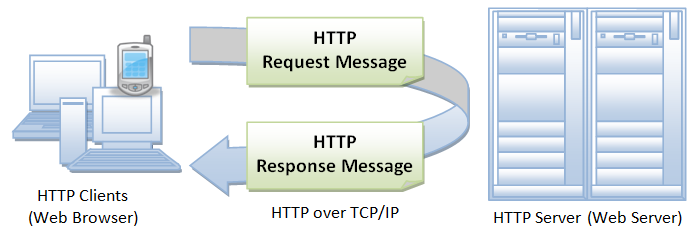
\includegraphics[width=\textwidth,keepaspectratio=true]{images/http.png}
  \caption[Hai loại thông điệp HTTP]{Hai loại thông điệp \acrshort{http}\protect\footnotemark}
  \label{fig:http}
\end{figure}
\footnotetext{Nguồn: https://www.ntu.edu.sg/home/ehchua/programming/webprogramming/HTTP\_Basics.html}
\textbf{Thông báo yêu cầu HTTP} (HTTP request) được gửi từ người dùng đến máy chủ để yêu cầu máy chủ thực thi một hành động nào đó. \acrshort{http} request gồm các thành phần:
\begin{itemize}
    \item \textbf{Dòng bắt đầu (start line)} ví dụ như \colorbox{gray!30}{\texttt{POST / HTTP/1.1}}, \colorbox{gray!30}{\texttt{GET /1-duck.png HTTP/1.0}},\\\colorbox{gray!30}{\texttt{HEAD /items.html?productId=1337 HTTP/1.1}}, \colorbox{gray!30}{\texttt{OPTIONS /index.html HTTP/1.0}}. Dòng bắt \\đầu này bao gồm 3 thành phần:
        \begin{itemize}
            \item \textbf{Phương thức \acrshort{http} (HTTP method)} dùng để mô tả hành động sẽ được thực thi bởi request đó. Những phương thức thường gặp là \texttt{GET, POST, PUT, HEAD, OPTIONS},...
            \item \textbf{Đối tượng yêu cầu (request target)} thường là một đường dẫn \acrshort{url} hoặc đường dẫn tuyệt đối đến tài nguyên trên máy chủ, nơi mà máy chủ sẽ thực hiện hành động đã yêu cầu.
            \item \textbf{Phiên bản HTTP} định nghĩa cấu trúc của phần còn lại của request, đồng thời đóng vai trò chỉ thị phiên bản \acrshort{http} mà response sẽ dùng.
        \end{itemize}
    \item \textbf{Tiêu đề (headers)} của một request gồm nhiều dòng, mỗi dòng được thiết kế theo cấu trúc quy định: một chuỗi kí tự (phân biệt hoa-thường) và giá trị có cấu trúc tương ứng tùy theo từng chuỗi, phân cách nhau bởi dấu hai chấm. Các dòng tiêu đề này được phần làm 3 loại chính như Hình \ref{fig:HTTP-request-headers} sau:
        \begin{figure}[H]
          \centering
            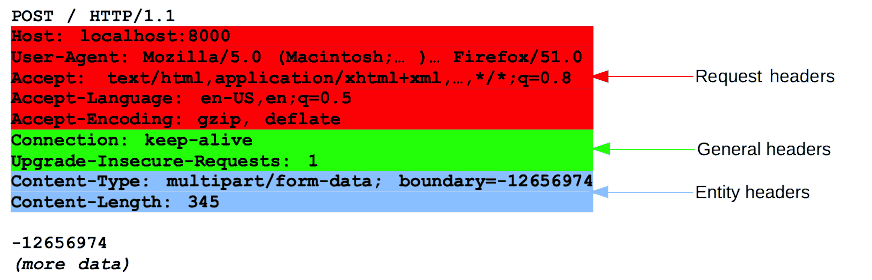
\includegraphics[width=\textwidth,keepaspectratio=true]{images/HTTP-request-headers.png}
          \caption[Các thành phần trong tiêu đề của một \acrshort{http} request]{Các thành phần trong tiêu đề của một \acrshort{http} request \protect\footnote{\href{https://developer.mozilla.org/en-US/docs/Web/HTTP/CSP}{https://developer.mozilla.org/en-US/docs/Web/HTTP/CSP}
          \label{fig:HTTP-request-headers}
        \end{figure}
        \begin{itemize}
            \item \textbf{Tiêu đề chung (general headers)} gồm những quy tắc/phiên bản được áp dụng lên toàn bộ request.
            \item \textbf{Tiêu đề request (request headers)} làm rõ request bằng việc đặc tả kĩ hơn về bối cảnh yêu cầu cũng như những giới hạn có điều kiện trên request đó.
            \item \textbf{Tiêu đề thực thể (entity headers)} gồm những quy tắc áp dụng lên phần nội dung (body) của request, nếu request không có nội dung thì phần tiêu đề cũng không có những tiêu đề thực thể này.
        \end{itemize}
    \item \textbf{Nội dung (body)} được phân cách với phần tiêu đề bởi một dòng trống. Phần nội dung này có thể có hoặc không, đa phần nó hiện diện trong những request có phương thức \texttt{POST} được gửi kèm theo biểu mẫu dữ liệu \acrshort{html}.
\end{itemize}
\textbf{Thông báo phản hồi HTTP} (HTTP response) được máy chủ trả về  cho người dùng, là câu trả lời cho hành động đã được yêu cầu bởi người dùng thông qua \acrshort{http} request. \acrshort{http} response gồm các thành phần tương tự như HTTP request. Các dòng tiêu đề trên \acrshort{http} response cũng được phần làm 3 loại chính như Hình \ref{fig:HTTP-response-headers} sau.
\begin{figure}[H]
  \centering
    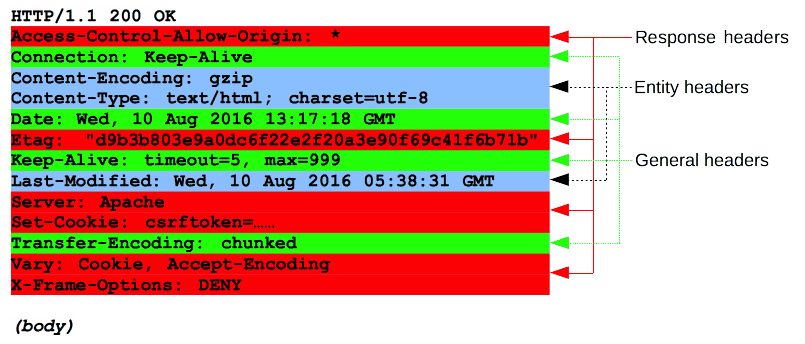
\includegraphics[width=\textwidth,keepaspectratio=true]{images/HTTP-response-headers.png}
  \caption[Các thành phần trong tiêu đề của một \acrshort{http} response]{Các thành phần trong tiêu đề của một \acrshort{http} response \protect\footnote{\href{https://developer.mozilla.org/en-US/docs/Web/HTTP/CSP}{https://developer.mozilla.org/en-US/docs/Web/HTTP/CSP}
  \label{fig:HTTP-response-headers}
\end{figure}

% TODO: có thế sẽ viết thêm về cả CSP và CORS?
% \subsection{Chính sách cùng nguồn gốc}
% Phần này trình bày khái niệm và những ngoại lệ của chính sách cùng nguồn gốc \parencite{sullivan2011web} \acrfull{sop}. Chính sách cùng nguồn gốc là một trong những khái niệm nền tảng trong lĩnh vực bảo mật trình duyệt web. Không có \acrshort{sop} thì mọi trang web trên internet đều có thể tiếp cần được thông tin bí mật của người dùng ở bất kì trang web nào khác. Việc khai thác các lỗ hổng bảo mật như \acrshort{xss}, \acrshort{sqli} (sẽ được làm rõ ở phần sau), \acrfull{xsrf},... là cách thức chủ yếu để vượt qua tính phòng thủ vốn có của \acrshort{sop}. \acrshort{sop} là một sự đồng thuận cần thiết giữa những nhà cung cấp trình duyệt web (như Microsoft, Apple, Google, Mozilla, Opera) trong việc giới hạn chức năng cũng như quyền hạn của các đoạn mã kịch bản (scripting code) trên trình duyệt của \textbf{người dùng} (client-side, phân biệt với phía máy chủ - server-side). \acrshort{sop} quy định rằng khi người dùng đang truy cập một trang web X nào đó trên trình duyệt, những đoạn mã của trang web X đó chỉ được phép đọc và ghi nội dung xuống một trang web Y khác (và ngược lại) nếu cả hai trang web X và Y có cùng nguồn gốc (origin). Hai trang web có cùng nguồn gốc ở đây có nghĩa là giống hệt nhau về ba thành phần: giao thức tầng ứng dụng của trang web (\acrshort{http}, \acrshort{https}), cổng TCP (thường là cổng 80 cho giao thức \acrshort{http} và cổng 443 cho giao thức \acrshort{https}), và tên miền của hai trang web (ví dụ \texttt{www.example.com} hay \texttt{www.google.com}).
% \begin{figure}[H]
%   \centering
%     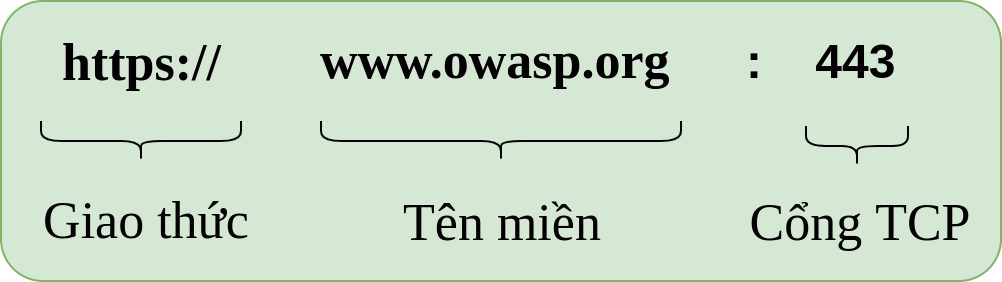
\includegraphics[width=0.6\textwidth,keepaspectratio=true]{images/origin-definition.png}
%   \caption{Các thành phần của nguồn gốc (origin) của một trang web}
%   \label{fig:origin-definition}
% \end{figure}
% Ví dụ về việc so sánh nguồn gốc giữa các trang web khác nhau được thể hiện như Bảng \ref{tab:SOP-example} sau.
% \begin{table}[ht]
%     \centering
%     \caption{Minh họa việc so sánh nguồn gốc với trang web \texttt{https://drive.google.com/my-drive}}
%     \label{tab:SOP-example}
%     \begin{tabular}[t]{lcc}
%         \toprule[1pt]\midrule[0.3pt]
%             \textbf{Đường dẫn URL}&\textbf{Kết quả}&\textbf{Lý do}\\
%         \midrule
%             \texttt{https://drive.google.com/your-drive}&Cùng nguồn gốc&Chỉ khác đường dẫn\\
%             \addlinespace
%             \texttt{https://drive.google.com/my-drive/my-docs}&Cùng nguồn gốc&Chỉ khác đường dẫn\\
%             \addlinespace
%             \texttt{http://drive.google.com/my-drive}&Không cùng nguồn gốc&Khác giao thức\\
%             \addlinespace
%             \texttt{https://drive.google.com:444/my-drive}&Không cùng nguồn gốc&Khác cổng\\
%             \addlinespace
%             \texttt{https://mail.google.com/my-drive}&Không cùng nguồn gốc&Khác tên miền\\
%         \midrule[0.3pt]\bottomrule[1pt]
%     \end{tabular}
% \end{table}
% Bên cạnh việc chỉ cho phép tương tác về mặt dữ liệu với những trang web có cùng nguồn gốc thì \acrshort{sop} cũng có một số ngoại lệ, cho phép ứng dụng web vượt qua \acrshort{sop} một cách có kiểm soát. Điều này giúp ứng dụng web trở nên uyển chuyển, giàu nội dung, đa chức năng và dễ hiện thực các chức năng đó hơn. Một số thẻ \acrshort{html} ngoại lệ được vượt qua \acrshort{sop} tiêu biểu có thể kể đến.
% \begin{itemize}
%     \item \texttt{<script src="..."></script>}
%     \item \texttt{<link rel="stylesheet" href="...">}
%     \item \texttt{<img src="...">, <video>, <audio>, <object>, <applet>}
%     \item \texttt{<iframe src="...">, <frame>}
% \end{itemize}
% Những thẻ \acrshort{html} kể trên (cùng với một số ngoại lệ đặc thù khác) được phép tải về và thực thi mã nguồn/hình ảnh/video từ địa chỉ web được đặc tả trong thuộc tính \texttt{src}, \texttt{href},... cho dù những địa chỉ web đó có thể không có cùng nguồn gốc với trang web nguồn.

\chapter{Một số lớp lỗ hổng bảo mật trên ứng dụng web}
% TODO: mô tả thêm những hướng có thể dựa trên background ở trên nhưng chỉ tập trung vào application layer và HTTP request/response
Trong phạm vi hiện thực công cụ, tôi chỉ tập trung vào việc tìm hiểu và phát hiện hai lỗ hổng bảo mật ở tầng ứng dụng của ứng dụng web, \acrfull{lfi} và time-based \acrlong{sqli} (SQLI). Đầu tiên, tôi sẽ trình bày về \acrfull{lfi}, một trong những lỗ hổng bảo mật phổ biến nhất trên ứng dụng web, luôn góp mặt trong top 10 lỗ hổng nguy hiểm nhất theo OWASP \parencite{owasp-top-10} nhiều năm gần đây. Nội dung phần này bao gồm làm rõ khái niệm \acrshort{lfi} và phân tích các kĩ thuật khai thác lỗ hổng bảo mật này.
\section{Local File Inclusion}
% https://www.rcesecurity.com/2017/08/from-lfi-to-rce-via-php-sessions/?fbclid=IwAR1VcA--iI7uRzwcqGk9JdcgHFZugVVNA1X2bLTSahRMhJy8Dk69gflKi8k
% https://outpost24.com/blog/from-local-file-inclusion-to-remote-code-execution-part-1
Lỗ hổng \acrfull{lfi} \parencite{portswigger-directory-traversal, sullivan2011web}, còn có tên khác là Directory Traversal, là lỗ hổng bảo mật trên ứng dụng web cho phép tin tặc đọc một vài tập tin nhạy cảm trên máy chủ mà ứng dụng web đang chạy trên. Những tập tin này có thể là mã nguồn, hình ảnh, dữ liệu hoặc thậm chí cả những tập tin hệ thống nhạy cảm. Trong một vài trường hợp xử lí phân quyền không tốt ở phía máy chủ, tin tặc còn có thể tạo thêm tập tin mới gây nên sự thay đổi dữ liệu và hành vi của ứng dụng, hoặc hắn có thể thực thi mã (\acrshort{rce}) từ phía máy chủ để chiếm quyền điều khiển hệ thống. Đoạn mã \ref{lst:php-lfi} dưới đây mô tả một điểm cuối của trang web ``\texttt{http://vuln-web.com/}'' có lỗ hổng \acrshort{lfi}.
\begin{lstlisting}[style=PHP, label={lst:php-lfi},caption={Đoạn mã PHP có lỗ hổng Local File Inclusion}]
/**
* Get the filename from a GET input
* Example - http://vuln-web.com/?file=filename.php
*/
$file = $_GET['file'];

/**
* Unsafely including the file
* Example - filename.php
*/
include('directory/' . $file);
\end{lstlisting}
Bằng cách nhận vào tham số \texttt{\$file} từ đường dẫn \acrshort{url}, máy chủ web trực tiếp trả về nội dung tập tin có tên \texttt{filename.php} trong thư mục hiện tại như trong ví dụ trên. Tin tặc có thể lợi dụng sơ hở từ câu lệnh \texttt{include('directory/' . \$file);} để trực tiếp đọc bất kì tập tin nào bằng cách sử đường dẫn tương đối, kết hợp tiền tố ``../'' (hoặc ``..\textbackslash'' đối với các máy chủ web dùng hệ điều hành Windows Server) để tham chiếu tới thư mục cha của thư mục hiện tại cộng với tên tập tin để đọc nội dung của tập tin đó, ví dụ như ``\texttt{http://vuln-web.com/?file=../../etc/passwd}''. Hình \ref{fig:lfi-payloads} sau đây minh họa một số vector tấn công (payload) dùng để đọc tập tin ``\textbf{passwd}'' trong đường dẫn \textbf{/etc/} trong các máy chủ web Unix.
\begin{figure}[H]
  \centering
    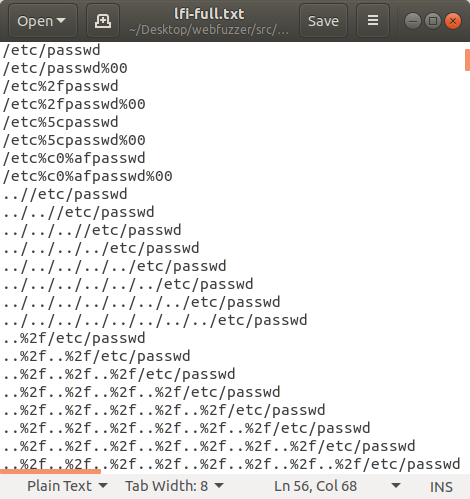
\includegraphics[width=0.7\textwidth,keepaspectratio=true]{images/lfi-payloads.png}
  \caption{Một số payload khai thác lỗ hổng \acrshort{lfi}}
  \label{fig:lfi-payloads}
\end{figure}
\textbf{/etc/passwd} là tập tin chứa danh sách tài khoản người dùng trên máy chủ web dùng hệ điều hành Unix, tập tin này bắt đầu bằng chuỗi ``\texttt{root:x}'' và chứa nhiều thông tin quan trọng như tên, địa chỉ email, đường dẫn tuyệt đối đến thư mục home trên đĩa cứng, ID của quyền (hoặc nhóm quyền) của người dùng đó,..., cung cấp cho tin tặc nhiều thông tin quý giá khi bắt đầu xâm nhập vào hệ thống. Do ta không biết độ sâu của thư mục ứng dụng web so với đường dẫn gốc (root directory) của hệ điều hành nên ta phải thử truy vấn đến từng tầng thư mục cha của thư mục hiện hành đến khi chạm tới thư mục gốc sau đó truy cập đến tập tin \textbf{/etc/passwd} như ví dụ trong Hình \ref{fig:lfi-payloads}.
\section{Time-based Structured Query Language Injection}
Hầu hết các kĩ thuật tấn công ứng dụng web đều tuân theo mô-típ đánh lừa ứng dụng web để thực hiện những hành động nguy hiểm thay tin tặc. Tin tặc không thể lấy được cookies của người dùng một cách chính quy nhưng có thể đánh lừa để trình duyệt web nạn nhân cung cấp cho hắn thông qua lỗ hổng \acrlong{xss} (\acrshort{xss}). Tin tặc cũng không thể tùy tiện truy xuất bất cứ tập tin nào trên máy chủ web nhưng hắn có thể lừa ứng dụng web làm việc đó thông qua lỗ hổng \acrshort{lfi}. Tương tự, tin tặc không thể trực tiếp truy cập và trích xuất cơ sở dữ liệu của ứng dụng web nhưng hắn có thể lừa ứng dụng web làm việc đó thông qua lỗ hổng \acrfull{sqli}. Phần này trình bày về khái niệm lỗ hổng \acrshort{sqli} nói chung và time-based \acrshort{sqli} nói riêng.\par
Lỗ hổng \acrfull{sqli} \parencite{li2011survey,sullivan2011web} cho phép tin tặc can thiệp vào các câu truy vấn \acrshort{sql} mà ứng dụng web dùng để tương tác với cơ sở dữ liệu. Thông thường việc này sẽ cho phép tin tặc đọc những dữ liệu mà hắn không có quyền, ví dụ như dữ liệu của những người dùng khác trong ứng dụng hoặc kể cả những dữ liệu mà ứng dụng đó không có quyền truy cập. Trong nhiều trường hợp tin tặc còn có thể sửa đổi hoặc sao chép (dump) những dữ liệu này, dẫn đến rủi ro bị đánh cắp dữ liệu và những hậu quả lâu dài cho nhà cung cấp ứng dụng web. Trong một vài điều kiện đặc biệt hơn, tin tặc còn có thể leo thang một cuộc tấn công \acrshort{sqli} để thỏa hiệp máy chủ ứng dụng web đang vận hành hoặc thực hiện một cuộc tấn công từ chối dịch vụ (\acrshort{dos} - \acrlong{dos}). Đoạn mã \ref{lst:php-sqli} sau đây\footnote{\href{http://websec.fr/level01/source.php}{Nguồn: http://websec.fr/level01/source.php}} là một ví dụ.
\begin{lstlisting}[style=PHP, label={lst:php-sqli},caption={Đoạn mã PHP có lỗ hổng SQL Injection}]
public function doQuery($injection) {
    $pdo = new SQLite3('database.db', SQLITE3_OPEN_READONLY);
    
    $query = 'SELECT id,username FROM users WHERE id=' . $injection . ' LIMIT 1';
    $getUsers = $pdo->query($query);
    $users = $getUsers->fetchArray(SQLITE3_ASSOC);

    if ($users) {
        return $users;
    }

    return false;
}
\end{lstlisting}
Câu truy vấn \acrshort{sql} trong ví dụ trên sẽ trả về cho người dùng giá trị của hai trường \texttt{id} và \texttt{username} của bản ghi đầu tiền trong bảng \texttt{users} có trường \texttt{id} bằng giá trị của tham số \texttt{\$injection} được truyền vào. Thông thường giá trị này thường là những chuỗi hoặc những con số có định dạng cụ thể, phục vụ cho việc truy vấn thông tin người dùng. Thông qua giao diện web hoặc \acrshort{http} request, tin tặc có thể can thiệp vào ứng dụng web và chỉnh sửa tùy ý nội dung của tham số \texttt{\$injection}. Ví dụ trong trường hợp giá trị tham số này là ``\colorbox{gray!30}{\texttt{1'; DROP TABLE users; -{}-'}}'', câu truy vấn trở thành\\
\colorbox{gray!30}{\texttt{SELECT id,username FROM users WHERE id='1'; DROP TABLE users; -{}-'}}\\
Sau khi truy vấn giá trị \texttt{id} và \texttt{username} của bản ghi có trường \texttt{id = 1} thì câu truy vấn \acrshort{sql} trên sẽ xóa toàn bộ nội dung (drop) bảng \text{users} trong cơ sở dữ liệu của ứng dụng. Bằng cách  thực hiện nhiều câu truy vấn nối tiếp hoặc lồng nhau (nested queries), đóng mở nháy đơn, sử dụng chú thích (-{}-) phù hợp với mã nguồn của trang web mà tin tặc có thể khai thác lỗ hổng \acrshort{sqli} này và gây ra hậu quả to lớn như thay đổi cấu trúc lược đồ quan hệ như ví dụ trên.\par
Lớp lỗ hổng \acrshort{sqli} có nhiều loại được phân ra dựa trên cách thức và mục tiêu tấn công \parencite{sqli-classification}, trong phạm vi luận văn này, tôi chỉ tập trung phát hiện lỗ hổng time-based \acrshort{sqli}. Time-based \acrshort{sqli} là kĩ thuật khai thác lỗ hổng \acrshort{sqli} bằng cách sử dụng những câu truy vấn đặc biệt, buộc hệ quản trị cơ sở dữ liệu phải chờ một khoảng thời gian trước khi trả về kết quả truy vấn cho ứng dụng, dựa vào thời gian phản hồi của câu truy vấn, ta có thể nhận định sự tồn tại của lỗ hổng này. Mục đích của việc kiểm thử lỗ hổng này không chỉ có vậy, việc khai thác thành công time-based \acrshort{sqli} trên những điểm cuối của một ứng dụng web còn có nghĩa là điểm cuối này cho phép truy vấn liên tiếp, lồng nhau, hoặc phát hiện được một số phần tử trong danh sách đen cũng như danh sách trắng của bộ lọc dữ liệu đầu vào, những nhận định này là cơ sở để tấn công sâu hơn vào ứng dụng web đó. Việc khai thác bằng kĩ thuật này phụ thuộc các hàm hoãn thời gian của mỗi hệ quản trị cơ sở dữ liệu khác nhau, cụ thể đối với MySQL ta dựa vào hàm \texttt{sleep} và \texttt{benchmark}, đối với Microsoft SQL Server là hàm \texttt{waitfor delay} và \texttt{waitfor time}, đối với Postgres SQL là \texttt{pg\_sleep},...

\input{technology/technology}
\chapter{Xu hướng tấn công ứng dụng web hiện nay và hướng phát triển ứng dụng webfuzzer}
\section{Xu hướng tấn công ứng dụng web hiện nay}
Bảo mật luôn là vấn đề hàng đầu trong nhiều lĩnh vực khác nhau của cuộc sống, đặc biệt trong lĩnh vực phần mềm máy tính/di động và ứng dụng web trong thời đại cách mạng công nghiệp 4.0 hiện nay. Những ứng dụng quan trọng liên quan đến tài chính, thông tin cá nhân của người dùng cũng đang được cung cấp rộng rãi bởi các ngân hàng, ví điện tử, mạng xã hội,... Tất cả điều đó hấp dẫn rất nhiều tin tặc và tổ chức tội phạm mạng, dẫn đến nguy cơ bị tấn công của các phần mềm nói chung và các ứng dụng web nói riêng. Đối với ứng dụng web, ngoài việc khai thác các lỗ hổng bảo mật ở tầng mạng như tấn công từ chối dịch vụ (denial of service - \acrshort{dos}), các phương pháp giả mạo bộ nhớ đệm (\acrshort{dns}/HTTP web server cache poisoning), chiếm tên miền phụ (subdomain takeover),..., tầng ứng dụng (đã được trình bày ở \textbf{Chương 3}) thì việc tấn công các ứng dụng web được lưu trữ ảo chung (virtual hosting) và khai thác những lỗ hổng 0-day và n-day mới của các công cụ, khung thức do bên thứ ba cung cấp cho ứng dụng web đang trở thành xu hướng. \par
Hiện nay, việc khai thác các lỗ hổng bảo mật trên một ứng dụng web còn có thể ảnh hưởng đến nhiều ứng dụng web khác thông qua sự phổ biến của các dịch vụ lưu trữ ảo. Lưu trữ ảo là một phương pháp cho phép lưu trữ (hosting) nhiều tên miền ứng dụng web trên một máy chủ vật lý. Việc sử dụng hosting ảo giúp tiết kiệm chi phí vận hành, tiết kiệm quỹ địa chỉ IPv4 sẵn có cũng như tạo điều kiện cho các dịch vụ hosting phát triển mạnh mẽ, cho phép họ dễ dàng cung cấp dịch vụ, quản lý việc hosting nhiều ứng dụng web khác nhau trên cùng một máy chủ vật lý, không cần phải đầu tư nhiều về phần cứng lẫn băng thông. Những máy chủ web thường dùng để triển khai hosting ảo là \textbf{Nginx}, \textbf{Apache}, hoạt động tốt trên các phiên bản của hai hệ điều hành máy chủ phổ biến nhất hiện nay là \textbf{Ubuntu Server} và \textbf{Windows Server}. Hai máy chủ web này lưu giữ mã nguồn và nội dung của các ứng dụng web trong quá trình vận hành dưới dạng các thư mục con (đối với \textbf{Apache}) hoặc các khối máy chủ (Nginx server block - đối với \textbf{Nginx}) tương ứng với các ứng dụng web riêng biệt, đồng thời cung cấp nhiều tính năng quản lý hosting, cải thiện hiệu năng, đảm bảo bảo mật cho các ứng dụng web trong cụm hosting ảo. Các tính năng trên thường xuyên được cải tiến, nâng cấp và bản thân \textbf{Apache} cũng như \textbf{Nginx} có chương trình trả thưởng cho các lỗ hổng bảo mật của họ (bug bounty program) rất hậu hĩnh, chúng ta có thể tạm yên tâm về khía cạnh bảo mật của các máy chủ web này nếu được cấú hình chuẩn bởi nhà cung cấp dịch vụ. Tuy nhiên việc sử dụng hosting ảo cũng tồn tại một số nhược điểm.
\begin{itemize}
    \item Sự tập trung nhiều ứng dụng web lại một chỗ gây ra rủi ro sụp đổ tại một điểm (single point of failure). Khi có sự cố về phần cứng máy chủ web hoặc một ứng dụng web trong cụm bị tấn công từ chối dịch vụ, khả năng đáp ứng người dùng của những ứng dụng web khác sử dụng chung dịch vụ hosting ảo cũng sẽ bị ảnh hưởng, do sử dụng chung máy chủ vật lý và băng thông. 
    \item Các rủi ro bảo mật cho các ứng dụng web dùng chung hosting chủ yếu đến từ chính các ứng dụng web trong cụm chứ không từ máy chủ web như \textbf{Nginx} hay \textbf{Apache}, và việc đảm bảo bảo mật cho mỗi ứng dụng web tham gia hosting chung phải do chính chủ sở hữu của từng ứng dụng web trực tiếp quản lý. Tuy dịch vụ hosting ảo có thể hỗ trợ việc này một phần, thông qua một số tính năng/bộ lọc giúp kiểm soát, giới hạn quyền truy cập, bảo mật cookies cũng như sao lưu và phục hồi dữ liệu của \textbf{Nginx} và \textbf{Apache}, nhưng về mặt lý thuyết, một ứng dụng web trong cụm hosting ảo bị xâm nhập thành công sẽ đồng nghĩa với việc tất cả các ứng dụng web còn lại đều có nguy cơ bị xâm nhập. Điều này có được là do tin tặc hoàn toàn có khả năng truy xuất nội dung (bên trong các thư mục con, khối máy chủ trong hệ thống) và can thiệp vào các dịch vụ vận hành của các ứng dụng web khác.
\end{itemize}
Hiện nay, các dịch vụ tường lửa ứng dụng web (web application firewalls - \acrshort{waf}) ngày càng được hoàn thiện, nhiều quy chuẩn (best practices) được đề ra trong cộng đồng lập trình viên và áp dụng rộng rãi trong nhiều ngôn ngữ lập trình và khung thức, công cụ nhằm chống lại việc khai thác những lỗ hổng bảo mật thường gặp của ứng dụng web (như \acrshort{dos}, \acrshort{sqli}, \acrshort{xss}, remote code execution - \acrshort{rce},...). Một vài ví dụ tiêu biểu có thể kể đến như các dịch vụ tường lửa ModSecurity, CloudFlare, Citrix, AppTrana,..., các thư viện mã hóa và làm sạch dữ liệu đầu vào (input sanitizer) trên các ngôn ngữ lập trình phổ biến như PHP (HTML Purifier\footnote{\href{http://htmlpurifier.org/}{Nguồn: http://htmlpurifier.org/}}, PHP Intrusion Detection System, PHP Password Lib, PHPSecLib), NodeJS (awesome-nodejs-security, thư viện Helmet của express framework), ReactJS (dompurify, xss, xss-filters), ESAPI\footnote{\href{https://www.owasp.org/index.php/Category:OWASP_Enterprise_Security_API}{Nguồn: https://www.owasp.org/index.php/Category:OWASP\_Enterprise\_Security\_API}}, AntiXSS\footnote{\href{https://documentation.help/Microsoft-AntiXSS/}{Nguồn: https://documentation.help/Microsoft-AntiXSS/}},... Trong bối cảnh đề cập ở trên, một trong những hướng tấn công đáng để thử cho những tin tặc là điều tra và khai thác các ứng dụng web có lỗi trong những cụm hosting ảo này. Việc này tuy có thể mất nhiều thời gian công sức hơn tìm và khai thác các lỗ hổng bảo mật trên ứng dụng web mục tiêu của ta nhưng nếu thành công thì hậu quả để lại khó có thể đong đếm được do có rất nhiều trang web của những tổ chức lớn đang sử dụng dịch vụ hosting ảo. Và thông thường, những ứng dụng web quan trọng của một tổ chức nào đó (ví dụ như \href{https://bkpay.hcmut.edu.vn/bkpay/home.action}{BKPay} hay \href{https://mybk.hcmut.edu.vn/stinfo/}{ứng dụng quản lý} điểm số, thông tin cá nhân của sinh viên và cán bộ công nhân viên trong trường,...) thường sẽ được hosting chung để tiện trong công tác quản lý, nâng cấp, bảo mật và bảo trì thường xuyên. Giả sử như một ứng dụng web có lỗ hổng bảo mật và bị khai thác thì các ứng dụng web quan trọng khác cũng chung hosting sẽ ngay lập tức có nguy cơ cực kì cao sẽ bị thỏa hiệp, dẫn đến những mất mát to lớn về tài chính, về sự vận hành của cả tổ chức cũng như lộ thông tin cá nhân của rất nhiều người. \par
Một hướng tấn công đặc biệt hiệu quả hiện nay là khai thác những lỗ hổng bảo mật 0-day và n-day. Lỗ hổng 0-day là các lỗ hổng bảo mật trên phần mềm, phần cứng hoặc firmware mà nhà cung cấp các sản phẩm này chưa biết để vá lỗi. Thuật ngữ 0-day có thể được hiểu là chính bản thân lỗ hổng hoặc những cuộc tấn công đầu tiên sử dụng lỗ hổng đó. Sau khi một cuộc tấn công 0-day đã được công khai, lỗ hổng được nhà cung cấp thừa nhận và đang tiến hành vá lỗi, các tin tặc có thể viết mã khai thác để tấn công các hệ thống/ứng dụng sử dụng các sản phẩm chưa được vá lỗi đó. Thuật ngữ 1-day hay n-day dùng để chỉ ra thời gian (số ngày) giữa lúc cuộc tấn công diễn ra so với thời điểm nhà cung cấp công bố lỗ hổng hoặc để ám chỉ những lỗ hổng 0-day đã biết nhưng chưa có mã khai thác trên những môi trường khác nhau (ví dụ lỗ hổng A đã được khai thác thành công trên trình duyệt web Firefox trên hệ điều hành Windows nhưng chưa có mã khai thác lỗi A trên Ubuntu hay Android). Trách nhiệm của nhà cung cấp là công bố lỗ hổng ngay sau thời gian quy định (ví dụ như 90 ngày sau khi lỗ hổng được báo cáo đối với Project Google Zero) hoặc ngay khi có bản vá lỗi để cảnh báo các cá nhân và doanh nghiệp đang sử dụng sản phẩm của mình có động thái cập nhật bản vá hoặc tự vệ nếu lỗ hổng vẫn chưa được vá. Đồng thời các nhà cung cấp cùng các nhà phân phối và quản trị viên dưới quyền có trách nhiệm to lớn phải vá lỗ hổng n-day đó càng nhanh càng tốt để giảm thiểu thiệt hại không đáng có cho người dùng. Khái niệm lỗ hổng bảo mật và phơi bày thông tin thường gặp (common vulnerabilities and exposures - \acrshort{cve}) và liệt kê điểm yếu thường gặp của phần mềm (common weakness enumuration - \acrshort{cwe}) cũng được hình thành từ quá trình phát hiện - tấn công - vá lỗi liên tục này. \acrshort{cve} là một danh sách các lỗ hổng bảo mật được đặt mã hiệu và định danh của từng lỗ hổng kèm theo ít nhất một tài liệu tham khảo liên quan về lỗ hổng đó đã được công bố công khai. Danh sách này cũng như trang web tra cứu các \acrshort{cve}\footnote{\href{https://www.cvedetails.com/}{Nguồn: https://www.cvedetails.com/}} và \acrshort{cwe}\footnote{\href{http://cwe.mitre.org/}{Nguồn: http://cwe.mitre.org/}} được duy trì để phục vụ cho cộng đồng bởi \href{http://cve.mitre.org/}{MITRE Corporation}. Mục đích của CVE là để hệ thống các lỗ hổng, thuận tiện cho việc chia sẻ thông tin cũng như điều tra về các lỗ hổng có liên quan trong quá khứ của một nhà cung cấp nào đó. \par
Lỗ hổng bảo mật 0-day có thể xuất hiện ở bất cứ phần mềm, hệ thống, công cụ, khung thức nào, từ phía người dùng lẫn phía máy chủ ứng dụng web. Những lỗ hổng lớn gây nhiều thiệt hại thường nằm ở các trình duyệt web phổ biến như Google Chrome, Firefox, Safari; các khung thức và hệ quản trị nội dung (content management system - \acrshort{cms}) như Telerik, WordPress, Joomla, Wix, Shopify,...; các máy chủ web và dịch vụ lưu trữ, điện toán đám mây như Nginx, Apache, Microsoft Azure, Amazon Web Service,... Bằng việc sử dụng các lỗ hổng n-day hoặc các \acrshort{cve} liên quan đên các sản phẩm trên, tin tặc có thể tổ chức tấn công hàng loạt các cá nhân/doanh nghiệp sử dụng các sản phẩm đó với phiên bản thích hợp, chưa cập nhật bản vá. Khả năng thành công của dạng tấn công này gần như là tuyệt đối trong trường hợp sản phẩm đang được vận hành có cùng phiên bản và môi trường mà sản phẩm đó đang chạy trên, dẫn đến những vụ lộ thông tin cá nhân, thay đổi giao diện (deface), chiếm tên miền phụ,... của một số lượng cực lớn các trang web. Tiêu biểu có thể kể đến một loạt 3 \acrshort{cve} rất nguy hiểm của Telerik Web UI\footnote{\href{https://www.cvedetails.com/vulnerability-list/vendor_id-14130/Telerik.html}{Nguồn: https://www.cvedetails.com/vulnerability-list/vendor\_id-14130/Telerik.html}} trong năm 2017 cho phép tin tặc tải lên bất kì tệp độc hại nào cũng như tự do thực thi mã trên các ứng dụng web sử dụng các phiên bản Teleril Web UI cũ, hay 10 \acrshort{cve} của Wordpress\footnote{\href{https://www.cvedetails.com/vulnerability-list.php?vendor_id=2337}{Nguồn: https://www.cvedetails.com/vulnerability-list.php?vendor\_id=2337}} trong năm 2019 thông qua việc khai thác lỗ hổng \acrshort{xss} và \acrshort{rce}.\par
Hai hướng tấn công phổ biến đã trình bày ở trên ngày càng tỏ ra hiệu quả và phổ biến hiện nay, một trong những điểm chung của hai cách thức trên là rất khó để có thể tự động hóa bởi công cụ. Không như các phương pháp quét hoặc thử sai khác, việc điều tra hosting ảo cũng như viết mã khai thác các \acrshort{cve} trên nhiều môi trường khác nhau phải được thực hiện bằng tay. Một điểm chung nữa là việc tấn công các ứng dụng web kém bảo mật trong cụm hosting ảo cũng như việc hình thành các \acrshort{cve} phần lớn đều bắt nguồn từ các lỗ hổng bảo mật ở tầng ứng dụng (đã được trình bày ở \textbf{Chương 3}) rồi được tổng quát hóa, định danh và phân loại theo dạng lỗ hổng và nhà cung câp sản phẩm tương ứng. Các lỗ hổng đó là cơ sở cho sự xuất hiện của rất nhiều vấn đề về bảo mật trên ứng dụng web, đồng thời các những phương pháp tự động hóa trong việc kiểm thử các lỗ hổng đó cũng đã có sẵn và ngày càng được hoàn thiện hơn bởi sự đóng góp của cộng đồng. Từ hai điểm chung và những phân tích trên, chúng tôi nhận thấy một trong những hướng hiệu quả và cấp thiết để hiện thực công cụ kiểm thử các ứng dụng web theo đề tài luận văn là tập trung phát hiện các lỗ hổng bảo mật ở tầng ứng dụng với khả năng tự động hóa càng cao càng tốt.
\section{Phạm vi và hướng phát triển ứng dụng webfuzzer}
Trong phạm vi luận văn tốt nghiệp này, tôi sẽ áp dụng phương pháp kiểm thử fuzzing dưới dạng kiểm thử hộp đen để hiện thực công cụ \textbf{webfuzzer}. Ngoài khả năng tự động hóa cao, việc áp dụng phương pháp này sẽ đem lại nhiều lợi ích khác.
\begin{itemize}
    \item Linh hoạt trong việc kiểm thử nhiều ứng dụng web sử dụng các công nghệ, mô hình, khung thức phát triển phần mềm khác nhau, cũng như cho phép kiểm thử số lượng lớn ứng dụng web trong một khoảng thời gian ngắn.
    \item Đơn giản hóa và chuẩn hóa việc kiểm thử các lỗ hổng bảo mật trên những ứng dụng web có thiết kế cao cấp và phức tạp. Những ứng dụng này thường có số lượng dòng code có thể lên đến hàng nghìn thậm chí hàng triệu dòng, việc kiểm thử mã nguồn đối với phương pháp hộp trắng hoặc hộp xám sẽ khó khăn hơn nhiều.
    \item Dễ dàng đạt được khả năng tự động hóa cao so với việc quét mã nguồn của ứng dụng. Nhìn chung quá trình phát triển công cụ bằng phương pháp này không yêu cầu kĩ năng lập trình cao hoặc những kĩ thuật nhận diện lỗ hổng quá đặc thù.
    \item Chủ yếu tập trung vào việc kiểm thử chức năng của ứng dụng, không quan tâm đến giao diện, hiệu năng hay trải nghiệm người dùng. Điều này giúp ta có mục tiêu rõ ràng và tiết kiệm công sức cho quá trình thiết kế, cải tiến các trường hợp kiểm thử. 
\end{itemize}
Tương tự như trong lĩnh vực kiểm thử phần mềm, việc áp dụng phương pháp kiểm thử fuzzing dưới dạng kiểm thử hộp đen trong quá trình kiểm thử bảo mật ứng dụng web cũng sẽ có một số hạn chế như sau.
\begin{itemize}
    \item Do không nắm được mã nguồn của ứng dụng web nên chiến thuật tốt nhất là ta chỉ nên tập trung kiểm tra những vị trí thường phát sinh lỗ hổng nhất, hoặc dò quét và vượt qua (bypass) cách thức phòng thủ của ứng dụng bằng việc thử sai và làm rối (tampering) dữ liệu kiểm thử.
    \item Số lượng trường hợp kiểm thử kết hợp với các kĩ thuật bypass đã biết là quá lớn, yêu cầu nhiều kinh nghiệm thực tế của người lập trình để chọn lọc và viết ra được một công cụ nhanh và ổn định, tối ưu hóa tài nguyên máy tính và thời gian thực thi. Ta buộc phải đánh đổi thời gian và tài nguyên đó hoặc chấp nhận kiểm thử trên một tập dữ liệu nhỏ hơn chỉ chứa những trường hợp thường gặp nhất.
    \item Lập trình viên cần thường xuyên cập nhật các trường hợp kiểm thử và kĩ thuật tấn công/phòng thủ mới để bổ sung vào công cụ.
\end{itemize}
Hơn nữa, vấn đề đạo đức nghề nghiệp phải luôn luôn được đặt lên trên hết. Trước và trong quá trình kiểm thử ta phải có thỏa thuận với nhà cung cấp ứng dụng web về mục đích và cách thức tiến hành của mình, hoặc, xác định rõ động cơ của bản thân là để phát hiện những lỗ hổng nguy hiểm và sẽ báo cáo lại với nhà cung cấp để họ vá lỗi, tăng cường bảo mật và bảo vệ quyền lợi của người dùng ứng dụng đó. Bên cạnh đó ta cũng cần phải lưu ý về vấn đề pháp lý của mỗi vùng lãnh thổ địa lý hoặc quy định của những nhà cung cấp khác nhau, cũng như trang bị một số hiểu biết nhất định để bảo vệ danh tính và sự riêng tư của bản thân khi tiến hành kiểm thử số lượng lớn các ứng dụng web xuyên quốc gia.\par
Trong quá trình tìm hiểu và so sánh giữa các phương pháp, công cụ kiểm thử bảo mật ứng dụng web hiện tại, chúng tôi nhận thấy sử dụng chức năng \texttt{Intruder} của Burp Suite là phương pháp phù hợp nhất để tự động hóa quá trình phát hiện các lỗ hổng bảo mật ở tầng ứng dụng của các ứng dụng web thông qua thông điệp \acrshort{http}. \texttt{Intruder} là chức năng triển khai tấn công ứng dụng web tự động, mạnh mẽ và dễ cấu hình. Chức năng này có thể được sử dụng thực hiện những cuộc tấn công với phạm vi trải dài từ đơn giản tới phức tạp, từ vét cạn (brute-force) mật khẩu, thư mục ứng dụng web đến phát hiện các lỗ hổng bảo mật web ở tầng ứng dụng bằng phương pháp fuzzing. 
Bên cạnh đó, chúng tôi cũng sử dụng thêm chức năng \texttt{Extender}\footnote{\texttt{Extender} là một tính năng của Burp Suite, cung cấp thư viện lập trình và cho phép người dùng tích hợp thêm các phần mở rộng (extension) viết bằng Java hoặc Python vào Burp Suite} của Burp Suite để hỗ trợ gửi đối tượng kiểm thử (request mẫu) được chọn về backend của webfuzzer. Hình \ref{fig:send-base-request-1} sau mô tả giao diện chính của chức năng \texttt{Intruder}.
\begin{figure}[H]
    \centering
        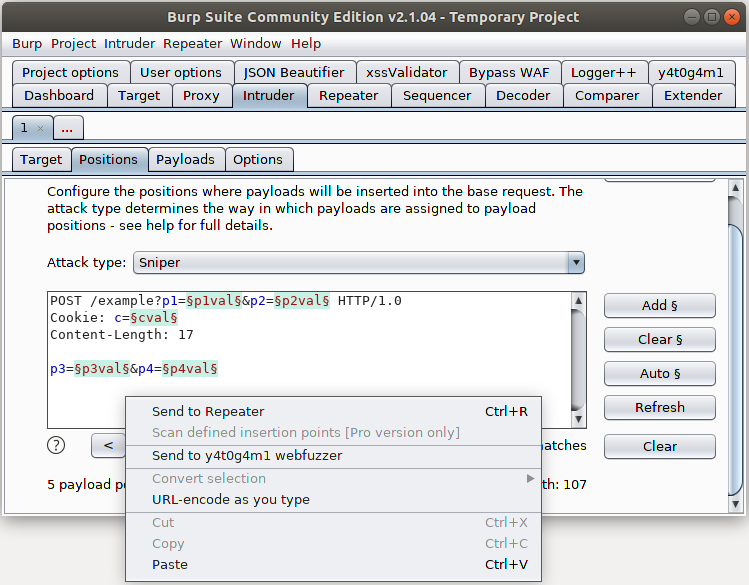
\includegraphics[width=0.8\textwidth,keepaspectratio=true]{images/send-base-request.png}
    \caption{Giao diện chính của chức năng Intruder}
    \label{fig:send-base-request-1}
\end{figure}
Giao diện chính của chức năng này gồm nhiều tab liền kề, mỗi tab được đánh số thứ tự, ứng với một \acrshort{http} request mẫu (base request) cần kiểm thử. Mỗi tab này gồm 4 tab phụ được mô tả như sau.
\begin{itemize}
    \item \textbf{Target} chứa thiết lập địa chỉ IP:port của ứng dụng web mục tiêu.
    \item \textbf{Positions} chứa những thiết lập của request mẫu cần kiểm thử, bao gồm các vị trí truyền tham số và kiểu tấn công.
    \item \textbf{Payloads} chứa các thiết lập liên quan đến tập vector tấn công (payload) kiểm thử. Tập payload này có thể được nhập từ tập tin trên máy, hoặc được sinh ra bằng một số phần mở rộng khác của Burp Suite, kèm theo các phương pháp tiền xử lí và encode payload thường dùng.
    \item \textbf{Options} chứa những thiết lập liên quan khác trong quá trình tấn công như thời gian chờ, các chuỗi và biểu thức chính quy để so trùng trên \acrshort{http} response trả về,...
\end{itemize}
Nhìn chung, chức năng này sử dụng cặp kí tự ``§'' để đánh dấu vị trí thay thế payload vào request mẫu để tạo thành requets kiểm thử, cụ thể việc sử dụng các danh sách payload và cách thức thay thế payload vào request mẫu như thế nào phụ thuộc vào kiểu tấn công của chức năng \texttt{Intruder}, gồm có \texttt{Sniper, Battering ram, Pitchfork} và \texttt{Cluster bomb}. Kiểu tấn công chúng tôi thường sử dụng nhất trong quá trình fuzzing bằng chức năng này là \texttt{Sniper}. Kiểu tấn công này chèn lần lượt từng payload trong danh sách vào từng vị trí thay thế payload trong request mẫu, do đó tổng số request kiểm thử được hình thành bằng tích số lượng payload nhân với số vị trí chèn payload trong request mẫu. Chúng tôi định ra hướng phát triển ứng dụng webfuzzer, hiện thực lại gần như đầy đủ chức năng \texttt{Intruder}, sử dụng kiểu tấn công \texttt{Sniper} vì những khuyết điểm của ứng dụng Burp Suite như sau.
\begin{itemize}
    \item Việc kiểm thử một request mẫu với nhiều loại lỗ hổng khá phiền phức, người dùng phải lần lượt sao chép các cấu hình kiểm thử cần thiết vào tab chứa request mẫu. Do đó, nhu cầu định ra một cấu hình kiểm thử mặc định rồi dùng để kiểm thử các request mẫu với nhiều lỗ hổng, cộng với một giao diện trực quan, thân thiện với người dùng hơn, là cần thiết.
    \item Burp Suite không tự động thực thi yêu cầu kiểm thử tiếp theo sau khi hoàn thành yêu cầu hiện tại. Do đó việc xây dựng một ứng dụng kiểm thử xoay quanh các yêu cầu kiểm thử là cần thiết. Việc này giúp quản lý và phân phối tài nguyên máy tính hợp lý hơn, người dùng có thể kiểm soát một lúc có bao nhiêu yêu cầu kiểm thử đang thực thi, tự động thực thi những yêu cầu kiểm thử đã tạo trong thời gian nhàn rỗi, đồng thời cắt giảm thời gian thực hiện các thao tác lặp đi lặp lại của họ so với sử dụng Burp Suite.
    \item Ứng dụng có thể dễ dàng được triển khai ứng dụng kiểm thử ở các dịch vụ cung cấp máy chủ ảo hóa (virtual private service - \acrshort{vps}. Việc kiểm thử bằng Burp Suite trên máy tính cá nhân (đặc biệt là tính năng \texttt{Intruder}) tiêu tốn khá nhiều tài nguyên máy tính, cản trở công việc, dẫn đến nhu cầu tách riêng chức năng này để triển khai trên một máy chủ độc lập. Việc này cũng giúp tránh được nguy cơ địa chỉ IP của máy tính cá nhân bị block theo vùng địa lý hoặc bởi các chính sách kiểm soát lưu lượng truy cập bởi ứng dụng web mục tiêu do gửi quá nhiều request đến trong một khoảng thời gian ngắn, giúp người kỹ sư kịp thời định ra phương hướng khác để tiếp cận mục tiêu.
    \item Việc lưu trữ kết quả kiểm thử ở Burp Suite cần phải được làm bằng tay, dẫn đến nhu cầu cần có một cơ sở dữ liệu để lưu trữ, hệ thống hóa những điểm cuối ứng dụng web có lỗ hổng kèm theo bằng chứng khai thác được lỗi trong quá trình kiểm thử tự động. Việc xây dựng một cơ sở dữ liệu như webfuzzer cũng là tiền đề để mở rộng ứng dụng trên lĩnh vực do thám (reconnaissance) các ứng dụng web mục tiêu trong tương lai.
    \item Việc xây dựng một ứng dụng web để kiểm thử thay vì sử dụng Burp Suite ở máy tính cá nhân còn giải quyết được nhu cầu làm việc chung và chia sẻ dữ liệu kiểm thử của nhiều người trong cộng đồng, hay hẹp hơn là tổ chức, công ty, thay vì chỉ một cá nhân đơn lẻ. Nhiều người có thể trực tiếp đóng góp vào cơ sở dữ liệu và truy vấn thông tin bằng cách sử dụng ứng dụng webfuzzer thay vì Burp Suite ở máy tính cá nhân.
\end{itemize}
Chúng tôi hiện thực ứng dụng webfuzzer để khắc phục các khuyết điểm trên của Burp Suite. Cụ thể về phạm vi, chúng tôi chỉ hiện thực chức năng so trùng trên chuỗi, biểu thức chính quy và kiểm tra thời gian phản hồi request của ứng dụng web mục tiêu. Chúng tôi không hiện thực chức năng nâng cao kiểm thử đa luồng (multithread) như Burp Suite vì dễ bị chặn do vượt hạn mức request ở các ứng dụng web mục tiêu. Chúng tôi cũng không hiện thực chức năng encode đối với payload và \acrshort{url} vì payload kiểm thử đã được encode và áp dụng các hình thức làm rối và bypass sẵn.
% TODO: chỉnh lại hình ảnh cho đúng kiến trúc
% TODO: payload tiếng Việt là gì
\chapter{Yêu cầu và thiết kế hệ thống ứng dụng webfuzzer}
Chương này trình bày các yêu cầu cần đạt trong quá trình thiết kế - hiện thực và chi tiết kiến trúc của ứng dụng webfuzzer.
\section{Yêu cầu hiện thực}
Trong đề mục này, những yêu cầu tổng quan và chức năng của ứng dụng và cơ sở dữ liệu của webfuzzer sẽ được làm rõ. Công dụng chính của webfuzzer là để lưu trữ những điểm cuối ứng dụng web khả nghi, kiểm thử theo thiết lập có sẵn và lưu lại lịch sử kiểm thử chi tiết. Trong phạm vi luận văn này, chúng tôi chỉ tập trung vào giao diện người dùng (\acrfull{ui} - \acrshort{ui}), backend và cơ sở dữ liệu của ứng dụng webfuzzer, phần mở rộng Burp Suite đã được cung cấp và có tài liệu sẵn.
\subsection{Ứng dụng web}
Dưới đây là những yêu cầu tổng quan và chức năng của ứng dụng webfuzzer trong quá trình thiết kế và hiện thực backend và UI của ứng dụng webfuzzer.
\subsubsection{Về tổng quan}
\begin{enumerate}
    \item Khả năng tiếp cận\\
    Backend và UI phải dễ dàng được tiếp cận được từ phía phần mở rộng Burp Suite và người dùng. Người dùng có thể tiếp cận mọi chức năng, giao diện lập trình ứng dụng (\acrlong{api} - \acrshort{api}) của ứng dụng và trước mắt chưa cần thiết phải có hệ thống phân quyền hay hạn chế việc này.
    \item Khả năng mở rộng\\
    Cấu hình kiểm thử ở phía backend phải linh hoạt, có thể được chỉnh sửa và thêm loại lỗ hổng bảo mật mới có thể được phát hiện theo cách tương tự. UI của ứng dụng nên được viết theo kiểu hướng thành phần (component-based) để có thể dễ dàng mở rộng bằng việc tái sử dụng các thành phần tương tự đã được lập trình trước.
    \item Hiệu năng\\
    Thời gian thực hiện một yêu cầu kiểm thử càng xấp xỉ (hoặc nhanh hơn) kiểm thử trên Burp Suite càng tốt. UI phải uyển chuyển, cung cấp được đầy đủ thông tin cần thiết để người dùng tiến hành kiểm thử và kiểm tra kết quả. Thời gian trả về kết quả khi gọi API không quá 1 giây cho một request trong điều kiện bình thường.
\end{enumerate}
\subsubsection{Về chức năng}
\begin{enumerate}
    \item Nhận và hiển thị \acrshort{http} request mẫu nhận được từ phần mở rộng Burp Suite\\
    Backend phải nhận được \acrshort{http} request mẫu được gửi từ phần ứng dụng của Burp Suite và lưu vào cơ sở dữ liệu, đồng thời UI phải hiển thị được những request mẫu đó thông qua việc tương tác với API của webfuzzer.
    \item Tùy chỉnh được cấu hình kiểm thử ứng với mỗi loại lỗ hổng bảo mật\\
    Cấu hình kiếm thử đối với từng lọai lỗ hổng phải có thể chỉnh sửa được (ít nhất là từ phía backend), đồng thời phải cung cấp API trả về cấu hình kiểm thử để hiển thị trên UI.
    \item Tạo và thực thi yêu cầu kiểm thử\\
    Dựa vào request mẫu và cấu hình kiểm thử hiển thị trên UI, người dùng phải dễ dàng tạo được yêu cầu kiểm thử trên UI thông qua việc chọn request mẫu và những loại lỗ hổng bảo mật cần kiểm thử. Sau đó người dùng có thể xem lại các thông số đó và tiến hành thực thi yêu cầu tương ứng.
    \item Xem kết quả kiểm thử\\
    Người dùng có thể xem lại kết quả kiểm thử trên UI, bao gồm các thông số, trạng thái, kết quả của mỗi yêu cầu kiểm thử cụ thể, kèm theo danh sách các payload phát hiện được mỗi loại lỗ hổng (nếu có). Đồng thời người dùng có thể dễ dàng lọc riêng những yêu cầu kiểm thử dương tính để xem xét thay vì hiển thị cả những yêu cầu âm tính.
\end{enumerate}
\subsection{Cơ sở dữ liệu}
Dưới đây là những yêu cầu tổng quan và chức năng của ứng dụng webfuzzer trong quá trình thiết kế và hiện thực một cơ sở dữ liệu nhanh và bền vững, đáp ứng được lưu cầu lưu trữ và truy xuất dữ liệu từ phía backend.
\subsubsection{Về tổng quan}
\begin{enumerate}
    \item Hạn chế trùng lặp dữ liệu\\
    Cơ sở dữ liệu phải tránh được tối đa việc lưu trữ các bản ghi hoặc thông tin trùng lặp, giữ cho kích thước của cơ sở dữ liệu càng nhỏ càng tốt.
    \item Khả năng mở rộng\\
    Lược đồ quan hệ và dữ liệu lưu trữ trong cơ sở dữ liệu cần có khả năng mở rộng cao, đặc biêt là những thông tin có độ dài không xác định trước được như kết quả kiểm thử, độ dài của request mẫu,...
    \item Hiệu năng\\
    Các câu truy vấn tới cơ sở dữ liệu phải có thời gian phản hồi trong khoảng chấp nhận được trong điều kiện bình thường, sao cho thỏa điều kiện thời gian phải hồi khi gọi API không quá 1 giây cho mỗi lời gọi API ở phía backend.
    \item Khả năng tương thích\\
    Việc cấu hình cơ sở dữ liệu, thiết lập các kết nối (connections) và truy vấn (queries) nên được hiện thực dễ dàng và hiệu quả trên ngôn ngữ lập trình phần backend của webfuzzer.
\end{enumerate}
\subsubsection{Về chức năng}
Cơ sở dữ liệu phải lưu trữ được đầy đủ và chính xác các thông tin của request mẫu bao gồm điểm cuối ứng dụng web mục tiêu, phương thức \acrshort{http}, cookies (nếu có) và các headers được gửi đến từ phần mở rộng Burp Suite; tương tự đối với các yêu cầu kiểm thử và kết quả kiểm thử tương ứng (nếu có).
\section{Trường hợp sử dụng}
Webfuzzer tập trung chủ yếu vào ba trường hợp sử dụng (use case) chính sau:
\begin{itemize}
    \item Trường hợp sử dụng 1: Gửi request mẫu từ phần mở rộng Burp Suite
    \begin{table}[ht]
        \centering
        \caption{Trường hợp sử dụng 1}
        \label{tab:use-case-1}
        \begin{tabular}[ht]{lll}
            \toprule[1pt]\midrule[0.3pt]
                \textbf{Đối tượng tương tác}& &Người dùng, phần mở rộng Burp Suite, \acrshort{ui} webfuzzer\\
            \midrule
                \textbf{Ranh giới hệ thống}& &Máy tính cá nhân của người dùng\\
            \midrule
                {}& &Backend và \acrshort{ui} của ứng dụng webfuzzer đang họat động,\\
                \textbf{Điều kiện trước}{}& &phần mềm Burp Suite có cài đặt sẵn phần mở rộng\\
                {}& &và trình duyệt web có thiết lập proxy sẵn\\
            \midrule
                {}& &Người dùng chọn và gửi request mẫu cần kiểm thử đến\\
                \textbf{Luồng thực thi}& &địa chỉ IP:port của ứng dụng. Webfuzzer sẽ phân giải request đó,\\
                {}& &lưu vào cơ sở dữ liệu và hiển thị lên giao diện người dùng\\
            \midrule
                {}& &Request mẫu được hiển thị trong danh sách \\
                \textbf{Điều kiện sau}& &trên giao diện webfuzzer sau thao tác gửi request\\
                {}& &và làm mới từ người dùng\\
            \midrule[0.3pt]\bottomrule[1pt]
        \end{tabular}
    \end{table}
    \FloatBarrier
    \item Trường hợp sử dụng 2: Tạo yêu cầu kiểm thử một điểm cuối ứng dụng web
    \begin{table}[ht]
        \centering
        \caption{Trường hợp sử dụng 2}
        \label{tab:use-case-2}
        \begin{tabular}[ht]{lll}
            \toprule[1pt]\midrule[0.3pt]
                \textbf{Đối tượng tương tác}& &Người dùng, giao diện người dùng webfuzzer\\ 
            \midrule
                \textbf{Ranh giới hệ thống}& &Máy tính cá nhân của người dùng\\
            \midrule
                \textbf{Điều kiện trước}& &Backend và \acrshort{ui} của ứng dụng webfuzzer đang họat động\\
            \midrule
                {}& &Người dùng chọn request mẫu từ danh sách đang hiển thị,\\
                \textbf{Luồng thực thi}& &sau đó chọn loại lỗ hổng cần kiểm thử\\
                {}& &và nhấn nút ``\textbf{Create fuzz request}''\\
            \midrule
                \textbf{Điều kiện sau}& &Yêu cầu kiểm thử tương ứng xuất hiện\\
                {}& &trong trang \textbf{Result} trên giao diện webfuzzer\\
            \midrule[0.3pt]\bottomrule[1pt]
        \end{tabular}
    \end{table}
    \FloatBarrier
    \item Trường hợp sử dụng 3: Xem kết quả kiểm thử theo thời gian
    \begin{table}[ht]
        \centering
        \caption{Trường hợp sử dụng 3}
        \label{tab:use-case-3}
        \begin{tabular}[ht]{lll}
            \toprule[1pt]\midrule[0.3pt]
                \textbf{Đối tượng tương tác}& &Người dùng, giao diện người dùng webfuzzer\\ 
            \midrule
                \textbf{Ranh giới hệ thống}& &Máy tính cá nhân của người dùng\\
            \midrule
                \textbf{Điều kiện trước}& &Backend và \acrshort{ui} của ứng dụng webfuzzer đang họat động\\
            \midrule
                \textbf{Luồng thực thi}& &Người dùng chọn trang \textbf{Result} để xem kết quả kiểm thử\\
                {}& &hoặc chọn một yêu cầu cụ thể để xem chi tiết\\
            \midrule
                \textbf{Điều kiện sau}& &Người dùng xem được tổng quan và chi tiết kết quả của mỗi\\
                {}& &yêu cầu kiểm thử. Đồng thời cho phép người dùng tái hiện lại\\
                {}& &request gây lỗi trên điểm cuối ứng dụng web mục tiêu\\
            \midrule[0.3pt]\bottomrule[1pt]
        \end{tabular}
    \end{table}
\end{itemize}
Bảng \ref{tab:use-case-1} thể hiện trường hợp sử dụng đầu tiên, cụ thể là khi người dùng muốn gửi request mẫu cần kiểm thử đến ứng dụng để hiển thị trên giao diện người dùng webfuzzer. Người dùng chọn request mẫu và vị trí tham số theo nhu cầu kiểm thử trên phần mở rộng Burp Suite, sau đó gửi đến địa chỉ IP:port đang triển khai ứng dụng webfuzzer (sẽ được trình bày chi tiết ở \textbf{Phụ lục A}). Sau đó nội dung của request mẫu này sẽ được hiển thị trên giao diện để người dùng kiểm tra và tạo yêu cầu kiểm thử theo một số lỗ hổng bảo mật.\par
Bảng \ref{tab:use-case-2} thể hiện trường hợp người dùng muốn tạo yêu cầu kiểm thử một request mẫu cụ thể với một số loại lỗ hổng. Người dùng chỉ việc chọn request mẫu trong danh sách và đánh dấu loại lỗ hổng cần kiểm thử và nhấn nút ``\textbf{Create fuzz request}''. Yêu cầu kiểm thử sẽ được đưa vào hàng đợi thực thi, đồng thời trạng thái và kết quả kiểm thử theo thời gian của yêu cầu này sẽ được hiển thị trong trang \textbf{Result} trên giao diện ứng dụng.\par
Trường hợp sử dụng 3 được thể hiện trong Bảng \ref{tab:use-case-3}. Trong trường hợp này, người dùng có thể xem chung kết quả của một số yêu cầu kiểm thử gần đây nhất hoặc xem chi tiết kết quả của một yêu cầu bất kì theo thời gian thực bao gồm kết quả tổng quát, những payload/biểu thức chính quy phát hiện ra lỗi, đồng thời cho phép người dùng gửi lại request mẫu kèm theo những payload đó để tái hiện lại bằng chứng (\acrshort{poc}) mắc lỗi của ứng dụng web mục tiêu.
\section{Công nghệ sử dụng}
Đề mục này trình bày tóm tắt những ngôn ngữ lập trình, công nghệ, công cụ được chọn để hiện thực ứng dụng webfuzzer. Những công nghệ này được lựa chọn dựa trên những nghiên cứu nền trong quá trình thực hiện luận văn. Chúng tương thích, hỗ trợ lẫn nhau và thích hợp trong việc thỏa mãn những yêu cầu hiện thực đã đề ra.\par
\textbf{Node.js} là một nền tảng phát triển ứng dụng độc lập được xây dựng trên Javascript Runtime của trình duyệt Chrome, thường được sử dụng để xây dựng các ứng dụng web một cách nhanh chóng và dễ dàng mở rộng. Phần lõi bên dưới của Node.js được viết hầu hết bằng C++ nên tốc độ xử lý và hiệu năng khá cao. Nhìn chung Node.js là một nền tảng rất thích hợp trong việc nhanh chóng xây dựng những ứng dụng web đa chức năng với hiệu năng cao, thích hợp với các startup hay luận văn tốt nghiệp này vì những lý do sau.
\begin{itemize}
    \item Node.js chạy đa nền tảng phía Server, sử dụng kiến trúc hướng sự kiện (event-driven), cơ chế non-blocking I/O làm cho nó nhẹ và hiệu quả.
    \item Ứng dụng viết bằng Node.js có thể chạy được ở bất kỳ hệ điều hành Mac – Windows – Linux.
    \item Cộng đồng Node.js rất lớn, hơn một triệu ba trăm nghìn gói thư viện (package) được cung cấp hoàn toàn miễn phí trên trang \href{https://www.npmjs.com/}{\textit{https://www.npmjs.com/}}, hỗ trợ trải dài trên nhiều lĩnh vực lập trình từ đại trà đến đặc thù.
    \item Các ứng dụng Node.js đáp ứng tốt thời gian thực và chạy đa nền tảng, đa thiết bị.
\end{itemize}
\textbf{Express.js} là một khung thức nhỏ, linh hoạt được xây dựng trên nền tảng Node.js. Nhiều khung thức nổi tiếng trên nền Node.js hiện đang sử dụng Express.js như \textbf{Sails}, \textbf{Feathers},... Express.js được xây dựng dựa trên rất nhiều gói thư viện bổ trợ và cung cấp thêm nhiều tính năng để lập trình viên tốt hơn, không làm giảm tốc độ vốn có của Node.js. Trong phạm vi luận văn này, Express.js được sử dụng như một bộ định tuyến (routing), đảm nhiệm việc phản hồi thông tin lại cho người dùng khi họ gọi \acrshort{api} đến những điểm cuối của ứng dụng webfuzzer. Những yêu cầu này thuộc dạng HTTP request bao gồm đường dẫn \acrshort{api}, phương thức request (GET, POST, DELETE, PUT,...) và các tham số cần thiết theo định dạng dữ liệu đầu vào của mỗi \acrshort{api}. \par
\textbf{React.js} là một thư viện hỗ trợ lập trình giao diện người dùng phổ biến trên ngôn ngữ Javascript. Một ứng dụng React.js được xây dưng xung quanh các thành phần (component) với khả năng tái sử dụng cao, thay vì dựa vào bản mẫu (template) như các thư viện lập trình \acrshort{ui} khác, cho phép nhúng mã \acrshort{html} trong mã Javascript nhờ vào JSX. JSX có ba điểm nổi bật chính.
\begin{itemize}
    \item Nhanh hơn. JSX thực hiện nhiều biện pháp tối ưu hóa trong khi biên dịch sang mã Javacsript. Việc thực thi các mã JSX này tốn ít thời gian hơn so với một mã tương đương viết trực tiếp bằng Javascript.
    \item An toàn hơn. JSX được biên dịch trước khi chạy, giống như các ngôn ngữ tĩnh khác như Java, C++,... Vì thế các lỗi nếu có sẽ được phát hiện ngay trong quá trình biên dịch.
    \item Dễ sử dụng hơn. JSX được viết dựa trên Javascript, vì vậy rất dễ dàng để các lập trình viên Javascript như chúng tôi có thể hiểu và sử dụng.
\end{itemize}
\textbf{Burp Suite} \parencite{burpsuite} là một khung thức kiểm thử thâm nhập (penetration testing framework) ứng dụng web trên nền Java, được cung cấp và phát triển bởi PortSwigger và đã trở thành bộ công cụ tiêu chuẩn được dùng trong công nghiệp bởi những kĩ sư an toàn thông tin. Công cụ này hỗ trợ nhận diện lỗ hổng bảo mật và xác thực các véc tơ tấn công vào ứng dụng web.
\begin{figure}[H]
  \centering
    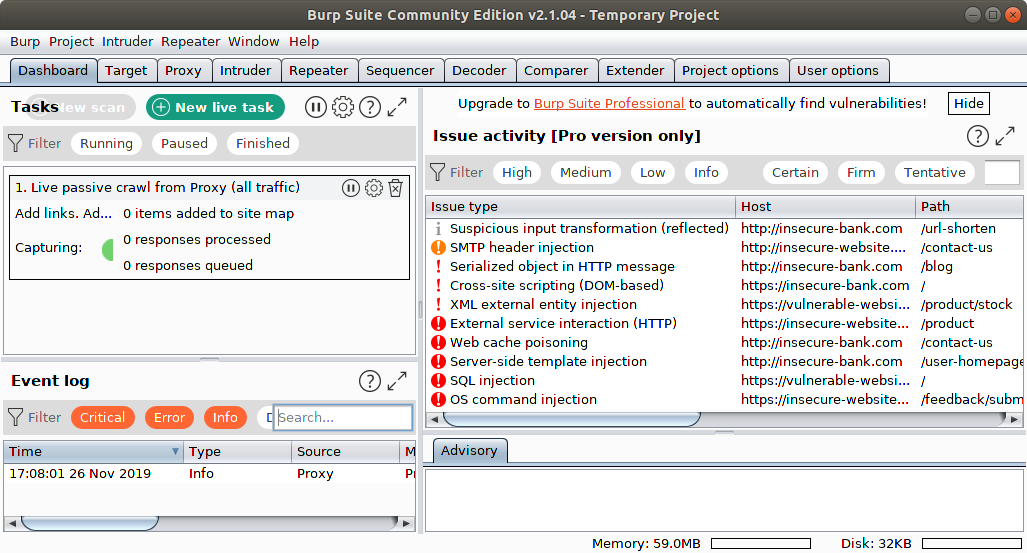
\includegraphics[width=\textwidth,keepaspectratio=true]{images/burp-suite-usage.png}
  \caption{Giao diện chính của công cụ Burp Suite}
  \label{fig:burp-suite-usage}
\end{figure}
Trong phạm vi luận văn này, Burp Suite vừa đóng vai trò như một proxy trung gian (interception proxy) can thiệp vào quá trình gửi \acrshort{http} request đến ứng dụng web mục tiêu, vừa đóng vai trò của một người trung gian (man in the middle - MITM) hỗ trợ chúng tôi phân tích, chỉnh sửa và chuyển tiếp request mẫu đó tới ứng dụng webfuzzer đồng thời cung cấp dữ liệu đối chứng trong quá trình kiểm thử tính đúng đắn và hiệu quả của ứng dụng.\par
\textbf{MySQL} là một hệ quản trị cơ sở dữ liệu mã nguồn mở, được sử dụng phổ biến trên thế giới vì tốc độ cao, sự ổn định, dễ sử dụng và khả năng hoạt động được trên nhiều hệ điều hành của nó. MySQL là một hệ quản trị cơ sở dữ liệu quan hệ, sử dụng ngôn ngữ truy vấn có cấu trúc (\acrlong{sql} - \acrshort{sql}). Đặc biệt MySQL có tính sẵn sàng và nhất quán cao theo mô hình CAP (Consistency - Availability - Partition tolerance), có sẵn thư viện tương tác được viết bằng Node.js và tương thích tốt với các hệ điều hành Windows, Linux, Mac OS X. Dựa vào những yếu tố trên, MySQL rất phù hợp trong việc hiện thực một cơ sở dữ liệu dựa trên những công nghệ và yêu cầu đã đề ra.
\section{Thiết kế kiến trúc hệ thống}
Đề mục này mô tả thiết kế chi tiết của kiến trúc hệ thống ứng dụng webfuzzer, bao gồm ba thành phần backend, \acrshort{ui} và cơ sở dữ liệu của ứng dụng.
\subsection{Backend}
Hai thành phần quan trọng nhất của backend là cấu hình - mô-đun kiểm thử và giao diện lập trình ứng dụng. Các cấu hình kiểm thử được xây dựng dựa trên những yếu tố cần thiết để kiểm thử bằng chức năng \textbf{Intruder} của Burp Suite. Giao diện lập trình ứng dụng được thiết kế theo kiểu RESTful \acrshort{api}, giao tiếp với \acrshort{ui} bằng các \acrshort{http} request/response. RESTful \acrshort{api} là một tiêu chuẩn được áp dụng để thiết kế các \acrshort{api} cho ứng dụng web, thông qua việc quy định cách sử dụng các phương thức \acrshort{http} (\texttt{GET, POST, PUT, DELETE…}) và cách định dạng \acrshort{url} sao cho phù hợp với chức năng của từng \acrshort{api} và quản lý tài nguyên chung của ứng dụng một cách có hệ thống.
\subsubsection{Cấu hình và mô-đun kiểm thử}
Dựa vào cách thức phát hiện lỗ hổng bằng thời gian phản hồi \acrshort{http} request và sự trùng khớp nội dung của response trả về, đối với mỗi loại lỗ hổng, chúng tôi xây dựng cấu hình kiểm thử bao gồm các thuộc tính sau. 
\begin{itemize}
    \item \textbf{label} là tên của lỗ hổng đang kiểm thử, dùng trong việc hiển thị trên giao diện và ghi nhật kí hoạt động.
    \item \textbf{time} là thời gian tối thiểu để một request kiểm thử trả về response, nếu thời gian phản hồi này lớn hơn giá trị của thuộc tính \textbf{time} thì được coi là phát hiện thành công lỗ hổng time-based \acrshort{sqli}. Thuộc tính này có thể là số giây cụ thể hoặc một chuỗi rỗng trong trường hợp người dùng không muốn giới hạn thời gian.
    \item \textbf{match} là một mảng các chuỗi để so trùng trên \acrshort{http} response, điểm cuối của ứng dụng web mục tiêu sẽ bị coi là có lỗ hổng nếu response trả về có chứa một trong những chuỗi này. 
    \item \textbf{payloadFile} là đường dẫn tập tin chứa các payload kiểm thử. Mặc định các payload này được chứa trong thư mục \texttt{payloads} trong thư mục gốc của mã nguồn backend và phân loại theo lỗ hổng bảo mật.
    \item \textbf{matchFile} là tập tin chứa các chuỗi để so trùng tương tự như thuộc tính \textbf{match} của cấu hình.
    \item \textbf{regex} là biểu thức chính quy dùng để phát hiện các chuỗi đáng ngờ trong \acrshort{http} response trả về, tương tự như thuộc tính \textbf{match}, điểm cuối của ứng dụng web mục tiêu sẽ bị coi là có lỗ hổng nếu response trả về khớp với các biểu thức chính quy này. Các biểu thức chính quy không chỉ bao gồm được các chuỗi để so trùng mà còn gồm cả các thông báo lỗi từ hệ điều hành, hệ quản trị cơ sở dữ liệu hay của chính ứng dụng web mục tiêu. Điều này gợi ý cho chúng tôi về những tiềm năng khai thác xa hơn, ngoài những lỗ hổng bảo mật ở tầng ứng dụng.
\end{itemize}
Việc thiết kế mô-đun kiểm thử sẽ được hiện thực dựa trên nguyên tắc hoạt động của chức năng \textbf{Intruder} trên Burp Suite, sử dụng loại tấn công \textbf{Sniper} như đã đề cập ở \textbf{Chương 4}, gồm các mô-đun nhỏ và các bước tuần tự như sau.
\begin{enumerate}
    \item Mô-đun phân tích request (\texttt{requestParser}) nhận vào \acrshort{http} request mẫu và cấu hình kiểm thử. Mô-đun này tiến hành đọc danh sách các payload từ thuộc tính \texttt{payloadFile} của cấu hình kiểm thử. Sau đó xác định từng vị trí thay thế payload riêng lẻ trong request mẫu (ở dạng chuỗi), được đánh dấu bằng cặp kí tự ``\$'' để thay thế lần lượt từng payload vào từng vị trí. Kết quả trả về của mô-đun này là một danh sách các \acrshort{http} request mẫu có chứa payload.
    \item Mô-đun xây dựng \acrshort{http} request kiểm thử (\texttt{requestBuilder}) nhận vào danh sách request mẫ có chứa payload ở trên. Mô-đun này lần lượt xây dựng \acrshort{http} request kiểm thử đầy đủ dựa trên các thành phần \texttt{url, headers, cookies, data, method} của từng request mẫu trong danh sách, sau đó lần lượt gửi các request kiểm thử này đến ứng dụng web mục tiêu.
    \item Các mô-đun kiểm thử (\texttt{fuzzer}) sẽ kiểm tra thời gian phản hồi và so trùng nội dung của \acrshort{http} response trả về dựa trên cấu hình kiểm thử để xác định khả năng có lỗ hổng của điểm cuối ứng dụng web mục tiêu. 
    \item Trong trường hợp mô-đun kiểm thử xác nhận được lỗ hổng từ quá trình phân tích response trả về như trên, mô-đun lưu trữ kết quả kiểm thử (\texttt{updateFuzzingLog}) sẽ được gọi. Mô-đun này đảm nhiệm việc lưu lại (hoặc cập nhật) loại lỗ hổng mà điểm cuối của ứng dụng web mục tiêu mắc phải kèm theo những payload phát hiện được lỗ hổng tương ứng vào cơ sở dữ liệu.
\end{enumerate}
\subsubsection{Giao diện lập trình ứng dụng - \acrshort{api}}
Giao diện lập trình ứng dụng của webfuzzer sẽ được điều hướng thông qua chức năng định tuyến (routing) được hỗ trợ bởi khung thức Express.js và hiện thực bằng các lớp trình điều khiển (controller class). Các lớp này cung cấp các phương thức (method) để tương tác với cơ sở dữ liệu, trả về thông tin và tiến hành kiểm thử ở phía backend. \acrshort{ui} của webfuzzer sẽ tạo \acrshort{http} request gọi đến đường dẫn \acrshort{api} kèm theo những tham số cần thiết, các phương thức này sẽ xử lý những request đó và trả về response dưới dạng đối tượng JSON. Các lớp trình điều khiển và các phương thức trong đó hoạt động độc lập với nhau, được phân loại theo chức năng như sau.
\begin{itemize}
    \item Lớp \textbf{BurpController} xử lý các yêu cầu liên quan đến \acrshort{http} request mẫu, bao gồm nhận request từ phía phần mở rộng Burp Suite và trả về danh sách các request mẫu đã lưu.
    \item Lớp \textbf{TargetController} đảm nhiệm việc tạo yêu cầu kiểm thử, truy vấn cấu hình kiểm thử và thông tin của các yêu cầu kiểm thử. Các phương thức trong lớp này không chỉ trả về một danh sách các yêu cầu kiểm thử được lọc ra theo nội dung tìm kiếm hoặc phân loại theo kết quả kiểm thử có lỗ hổng hay không mà còn có thể trả về thông tin chi tiết của một yêu cầu kiểm thử đơn lẻ.
    \item Lớp \textbf{FuzzController} cung cấp các phương thức thực thi yêu cầu kiểm thử theo ID hoặc một yêu cầu ngẫu nhiên đã được tạo.
\end{itemize}
Mỗi phương thức trong các lớp trình điều khiển này thực hiện những công việc tương ứng với chức năng của một \acrshort{api}. Cụ thể, Bảng \ref{tab:api-design} dưới đây mô tả kiến trúc giao diện lập trình ứng dụng ở phía backend của webfuzzer, được xây dựng dựa trên tiêu chuẩn RESTful.
\FloatBarrier
\begin{table}[ht]
    \centering
    \caption{Kiến trúc giao diện lập trình ứng dụng của webfuzzer backend}
    \label{tab:api-design}
    \begin{tabular}[ht]{cccl}
        \toprule[1pt]\midrule[0.3pt]
            \textbf{Lớp điều khiển}&\textbf{Tên phương thức}&\textbf{Đường dẫn API}&\textbf{Mô tả}\\ 
        \midrule
            {}&receiveTargetFromBurp&\colorbox{gray!30}{\texttt{POST /}}&Nhận request mẫu từ\\
            BurpController&{}&{}& phần mở rộng Burp Suite\\
            \addlinespace
            {}&getAllEndpoint&\colorbox{gray!30}{\texttt{GET /}}&Truy vấn danh sách các \\
            {}&{}&{}&request mẫu đã nhận\\
            \midrule[0.3pt]
            {}&createFuzzRequest&\colorbox{gray!30}{\texttt{POST /target}}&Tạo yêu cầu kiểm thử\\
            \addlinespace
            {}&retrieveRequestInfo&\colorbox{gray!30}{\texttt{GET /target}}&Truy vấn một yêu cầu\\
            {}&{}&{}& kiểm thử theo ID\\
            \addlinespace
            {}&getRequestList&\colorbox{gray!30}{\texttt{GET /target/list}}&Truy vấn danh sách các\\
            TargetController&{}&{}&yêu cầu kiểm thử\\
            \addlinespace
            {}&getVulnTypes&\colorbox{gray!30}{\texttt{GET /target/configs}}&Truy vấn danh sách\\
            {}&{}&{}&cấu hình kiểm thử\\
            \addlinespace
            {}&searchUrl&\colorbox{gray!30}{\texttt{GET /target/search}}&Lọc yêu cầu kiểm thử\\
            {}&{}&{}&theo \acrshort{url}\\
            \midrule[0.3pt]
            {}&executeFuzzRequest&\colorbox{gray!30}{\texttt{GET /fuzz}}&Thực thi một yêu cầu\\
            FuzzController&{}&{}&kiểm thử theo ID\\
            \addlinespace
            {}&executeSubmittedRequest&\colorbox{gray!30}{\texttt{GET}}&Thực thi một yêu cầu\\
            {}&{}&\colorbox{gray!30}{\texttt{/fuzz/free-request}}&kiểm thử đã tạo\\
        \midrule[0.3pt]\bottomrule[1pt]
    \end{tabular}
\end{table}
% TODO: Viết phần cấu trúc chương trình này nếu có thời gian
% \subsubsection{Cấu trúc chương trình}
% \begin{itemize}
%     \item Quản lý việc tương tác với cơ sở dữ liệu
%     \item 
% \end{itemize}
\subsection{Giao diện người dùng}
% \begin{enumerate}[label*=\arabic*.]
%     \item 
% \end{enumerate}
Giao diện của ứng dụng webfuzzer sẽ có hai trang web chính và thanh điều hướng để chuyển đổi qua lại giữa hai trang này. Thiết kế chi tiết kèm theo những \acrshort{api} mà các thành phần này sử dụng được mô tả như sau.
\begin{enumerate}
    \item Trang bảng điều khiển (Dashboard page) để người dùng tạo yêu cầu kiểm thử dựa trên \acrshort{http} request mẫu và cấu hình kiểm thử.
    \begin{itemize}
        \item Khung hiển thị danh sách \acrshort{url} các \acrshort{http} request mẫu để chọn. Danh sách này là kết quả trả về của việc gọi \acrshort{api} \texttt{GET /}, đồng thời có khung hiển thị nội dung của request mẫu đã chọn kèm theo các kí tự ``\$'' đánh dấu vị trí chèn payload như lúc gửi request mẫu từ chức năng \textbf{Intruder} của Burp Suite.
        \item Khung hiển thị và chọn các loại lỗ hổng bảo mật cần kiểm thử. Khung này gồm một danh sách các checkbox kèm theo tên lỗ hổng, người dùng có thể chọn một hay nhiều lỗi tùy theo nhu cầu kiểm thử. Danh sách các lỗ hổng này được trả về thông qua việc gọi \acrshort{api} \texttt{GET /target/configs}.
        \item Nút tạo yêu cầu kiểm thử cho phép người dùng tạo yêu cầu kiểm thử từ request mẫu và các lỗ hổng bảo mật đã chọn, gọi đến \acrshort{api} \texttt{POST /target}.
    \end{itemize}
    \item Trang kết quả kiểm thử (Result page) để người dùng thực thi và kiểm tra kết quả kiểm thử. Trang này cho phép người dùng xem thông tin chi tiêt của mỗi yêu cầu kiểm thử, đồng thời cho phép (tái) thực thi những yêu cầu đã tạo hoặc kiểm thử chưa hoàn tất.
    \begin{itemize}
        \item Thành phần chính của trang này là một bảng hiển thị thông tin tổng quan của một danh sách các yêu cầu kiểm thử được trả về từ \acrshort{api} \texttt{GET /target/list} hoặc \texttt{GET /target/search}.
        \item Mỗi hàng của bảng tương ứng với một yêu cầu kiểm thử. Cuối hàng có một nút nhấn để xổ xuống thông tin chi tiết của yêu cầu kiểm thử tương ứng, được truy vấn bằng \acrshort{api} \texttt{GET /target}.
        \item Ở cuối phần thông tin chi tiết của một yêu cầu kiểm thử, chúng tôi thêm một nút nhấn gọi đến \acrshort{api} \texttt{GET /fuzz} để (tái) thực thi yêu cầu kiểm thử đang chọn.
    \end{itemize}
    \item Thanh điều hướng (Sidebar) gồm tên ứng dụng webfuzzer, hai mục Dashboard và Result để điều hướng tới hai trang web chính của ứng dụng, kèm theo đường dẫn đến thư mục mã nguồn ứng dụng trên gitlab.
\end{enumerate}
Bên cạnh các thành phần chức năng chính trên, chúng tôi còn cần phải hiện thực thêm một số thành phần của \acrshort{ui} để cải thiện trải nghiệm người dùng (user experience - UX) như hệ thống thông báo đẩy (toast notification), giao diện ứng dụng đẹp mắt, dễ nhìn,...
\subsection{Cơ sở dữ liệu}
Nhằm đảm bảo mục đích lưu trữ các \acrshort{http} request mẫu, yêu cầu và kết quả kiểm thử, cơ sở dữ liệu của ứng dụng nên tách ra làm ba bảng chứa các đối tượng trên, tạm gọi lần lượt là các bảng \texttt{Endpoint, Request, Result}. Đối tượng chính là sẽ là bảng \texttt{Request}, chứa request mẫu, cấu hình (nếu có thể), các loại lỗ hổng cần kiểm thử, kết quả kiểm thử và một số thông tin khác. Một request mẫu có thể được kiểm thử nhiều lần tùy theo nhu cầu của người dùng nên ta tách \texttt{Endpoint} ra thành một bảng riêng, bảng \texttt{Request} lúc này sẽ có một trường tham khảo đến khóa chính của bảng \texttt{Endpoint} để tránh tình trạng dư thừa dữ liệu. Tương tự, bảng \texttt{Result} chứa kết quả kiểm thử cũng nên được tách riêng và thiết lập quan hệ khóa ngoài với bảng \texttt{Request} để dễ dàng thay đổi và mở rộng sau này.\par
Ngoài ra, có một phần dữ liệu cần lưu trữ thuộc kiểu đối tượng JSON (JavaScript Object Notation) ở phía backend, một kiểu dữ liệu mở trong Node.js và Javascript, được cấu thành từ nhiều cặp thuộc tính - giá trị. MySQL không hỗ trợ lưu trữ trực tiếp kiểu dữ liệu đối tượng JSON này nên các giá trị có kiểu này cần được chuỗi hóa ở phía backend trước khi gửi đến cơ sở dữ liệu. Vì lý do đó, một số trường tương ứng trong các bảng sẽ có kiểu chuỗi (string) để lưu trữ chúng.
\chapter{Hiện thực ứng dụng webfuzzer}
Chương này mô tả chi tiết hiện thực của kiến trúc hệ thống ứng dụng webfuzzer, bao gồm ba thành phần backend, \acrshort{ui} và cơ sở dữ liệu của ứng dụng.
\section{Backend}
\subsection{Phần mở rộng Burp Suite}
Phần mở rộng Burp Suite cho phép gửi \acrshort{http} request mẫu từ mô-đun \textbf{Intruder} của Burp Suite đến công cụ \textbf{webfuzzer} theo định dạng JSON như Đoạn mã \ref{lst:base-request-format} dưới đây, quá trình chọn và gửi request mẫu sẽ được trình bày ở \textbf{Phụ lục A} của luận văn.
\begin{lstlisting}[style=ES6, label={lst:base-request-format}, caption={Cấu trúc của một HTTP request mẫu được gửi từ phần mở rộng Burp Suite}]
{
    "python": { 
        "url":"http://testphp.vulnweb.com:80/search.php?test=query",
        "cookies":"",
        "headers":{ 
            "User-Agent":"Mozilla/5.0 (X11; Ubuntu; Linux x86_64; rv:71.0) Gecko/20100101 Firefox/71.0",
            "Accept":"text/html,application/xhtml+xml,application/xml; q=0.9,*/*;q=0.8",
            "Accept-Language":"en-US,en;q=0.5",
            "Accept-Encoding":"gzip, deflate",
            "Content-Type":"application/x-www-form-urlencoded",
            "Origin":"http://testphp.vulnweb.com",
            "DNT":"1",
            "Connection":"close",
            "Referer":"http://testphp.vulnweb.com/search.php?test=query",
            "Upgrade-Insecure-Requests":"1"
        },
        "data":{ 
            "searchFor":"\xa7a\xa7",
            "goButton":"go"
        },
        "method":"post"
    }
}
\end{lstlisting}
Chuỗi ``\texttt{\textbackslash xa7}'' trong trường \texttt{data.searchFor} biểu thị kí tự ``\$'' trong request mẫu. Các kí tự này thường nằm ở trường \texttt{data} hoặc \texttt{url} trong đoạn dữ liệu JSON để đánh dấu những vị trí chèn payload để ứng dụng web xử lí. 
\subsection{Cấu hình kiểm thử}
Điểm chung của những lỗ hổng bảo mật đã giới thiệu ở \textbf{Chương 3} là đều có thể bị khai thác bằng dữ liệu đầu vào từ phía người dùng. Vì thế, ta có thể phát hiện các lỗ hổng này bằng cách thử gửi nhiều dạng payload kiểm thử theo các tham số của \acrshort{http} request và phân tích phản hồi của máy chủ trong response trả về, việc làm này đặc biệt phù hợp với phương pháp fuzzing. Cụ thể giới hạn và phương pháp phát hiện của ứng dụng \textbf{webfuzzer} đối với từng lớp lỗ hổng như sau.
\begin{itemize}
    \item \acrshort{lfi}: ứng dụng tập trung phát hiển lỗ hổng này trên các máy chủ web dùng hệ điều hành nhân Unix. Cụ thể ứng dụng sẽ dùng những payload như Hình \ref{fig:lfi-payloads} để cố gắng đọc nội dung tập tin \texttt{/etc/passwd}. Ứng dụng sẽ kiểm tra \acrshort{http} response trả về xem có xuất hiện chuỗi ``\textbf{root:x}'' hoặc khớp với các biểu thức chính quy hay không để kết luận.
    \item Time-based \acrshort{sqli}: ứng dụng phát hiện tốt trên các ứng dụng web sử dụng các hệ quản trị cơ sở dữ liệu MySQL, Microsoft SQL Server và Postgres SQL bằng cách sử dụng các payload có chứa các hàm hoãn thời gian (đã đề cập ở \textbf{Phần 3.3}) của cả ba hệ quản trị cơ sở dữ liệu này, sau đó căn cứ vào thời gian phản hồi của \acrshort{http} response để kết luận.
\end{itemize}
Các payload, biểu thức chính quy, kĩ thuật tấn công, làm rối sử dụng trong ứng dụng được tổng hợp từ kinh nghiệm của chúng tôi và tổng hợp từ các kho lưu trữ (repository) mã nguồn trên GitHub \parencite{seclist-fuzzing,0verpwn-fuzzing}, từ nhiều blog chia sẻ cũng như write-up các thử thách cướp cờ (capture the flag - CTFs) của đàn anh đi trước trong ngành, từ các tweet được các kĩ sư bảo mật hàng đầu chia sẻ trên mạng xã hội Twitter,... Sau đó các payload này sẽ được chúng tôi chọn lọc và sửa đổi cho phù hợp với phương pháp kiểm thử của ứng dụng như sau.
\begin{itemize}
    \item Đối với các payload time-based \acrshort{sqli}, chúng tôi sử dụng các payload chứa hai loại hàm chính để hoãn thời gian thực hiện request. Cụ thể là hàm \texttt{sleep} (đối với MySQL, tương tự là \texttt{pg\_sleep} đối với PostgreSQL và \texttt{waitfor delay}, \texttt{waitfor time} đối với Microsoft SQL Server) và hàm \\\texttt{BENCHMARK(10000000,MD5('Y4T0G4M11337'))} để kéo dài thời gian thực hiện request đối với các ứng dụng web mắc lỗi này. Bên cạnh đó, với mỗi payload gốc, chúng tôi áp dụng thêm nhiều cách thức đóng ngoặc, chú thích để tránh gặp lỗi cú pháp khi thực thi đoạn mã SQL ở phía máy chủ.
    \item Đối với các payload \acrshort{lfi}, chúng tôi thu thập 8 payload mẫu với số lượng các chuỗi ``../'' tăng dần, nhằm tăng độ sâu của đường dẫn để tiếp cận được tập tin \texttt{/etc/passwd} của máy chủ. Từ 8 payload này, chúng tôi áp dụng các kĩ thuật làm rối riêng biệt để sinh ra 264 payload khác. Các kĩ thuật này bao gồm encode các chuỗi kí tự ``../'', ``..\textbackslash'' và ``..\textbackslash /'' theo các tập kí tự (charset) ít phổ biến như ``\texttt{..\%c0\%af}'', ``\texttt{..\%252f}'', ``\texttt{\%\%32\%65}'', ``\texttt{..\%\%32\%66}'',  ``\texttt{..\%25c1\%259c}'',... để vượt qua một số kĩ thuật lọc và làm sạch dữ liệu ở phía server-side của máy chủ ứng dụng web.
\end{itemize}
Cụ thể cấu hình được áp dụng trong ứng dụng và biểu thức chính quy áp dụng trong trường hợp phát hiện lỗi \acrshort{lfi} được thể hiện ở Đoạn mã \ref{lst:default-fuzz-config} dưới đây.
\begin{lstlisting}[style=ES6, label={lst:default-fuzz-config}, caption={Cấu hình kiểm thử mặc định}]
    let lfiRegex1 = /Warning: include\(|Warning: unlink\(|for inclusion \(include_path=|fread\(|Failed opening required|Warning: file_get_contents\(|Fatal error: require_once\(|Warning: file_exists\(/g;
    let lfiRegex2 = /java\.io\.FileNotFoundException|java\.lang\.Exception|java\.lang\ .IllegalArgumentException|java\.net\.MalformedURLException/g;
    let defaultFuzzConfig = {
        "1": { "label": "Local File Inclusion", "time": "", "match": ["root:x", "localhost"], "payloadFile": "lfi/lfi-full.txt", "matchFile": "", "regex": [lfiRegex1, lfiRegex2] },
        "2": { "label": "Time-based SQL Injection", "time": 10, "match": "", "payloadFile": "sqli/sqli-time-based.txt", "matchFile": "", "regex": [sqliRegex] },
        "3": { "label": "Remote Code Execution", "time": 10, "match": "", "payloadFile": "rce.txt", "matchFile": ["root:x", "371337", "99cebf4d56e5168a1915dd72213db9eb"], "regex": "" }
    }
\end{lstlisting}
Các cấu hình kiểm thử được quản lý bằng id dạng số, được định nghĩa và cung cấp từ phía backend thông qua \acrshort{api} để thống nhất giữa ba thành phần của hệ thống trong quá trình thực thi và lưu trữ. Các cấu hình này thường được chúng tôi sử dụng trong quá trình tìm lỗ hổng bảo mật trên các ứng dụng web bằng Burp Suite, chúng tôi sử dụng lại những cấu hình này cho việc kiểm thử ở ứng dụng webfuzzer để tiện so sánh và đánh giá kết quả hiện thực ứng dụng. Vì gặp khó khăn trong việc truyền biểu thức chính quy trong Node.js qua lại giữa \acrshort{ui} và cơ sở dữ liệu (bao gồm việc chuỗi hóa để lưu vào cơ sở dữ liệu và tái cấu trúc biểu thức chính quy để kiểm thử trên backend) nên hiện tại các cấu hình trên đang được thiết lập trong tập tin \texttt{globalConfig.js} trong thư mục gốc của mã nguồn backend, người dùng có thể sửa đổi các thuộc tính \texttt{payloadFile, match, time,...} trong tập tin trên theo nhu cầu kiểm thử. Ứng dụng chưa hỗ trợ việc thay đổi các thuộc tính này, linh động hóa quá trình thiết lập cấu hình kiểm thử từ phía \acrshort{ui}.\par
\subsection{Thiết lập các biến môi trường}
Các biến môi trường (environment variables) 
\FloatBarrier
\begin{table}[ht]
    \centering
    \caption{Danh sách các biến môi trường ở backend}
    \label{tab:env-variables-backend}
    \begin{tabular}[ht]{ccl}
        \toprule[1pt]\midrule[0.3pt]
            \textbf{Tên biến}&\textbf{Kiểu dữ liệu}&\textbf{Mô tả}\\ 
        \midrule
            SERVICE\_PORT&Integer&Cổng khởi chạy backend của ứng dụng\\
            \addlinespace
            mysqlConfig&Object&Các thiết lập để kết nối đến dịch vụ MySQL\\
            {}&{}&của hệ điều hành\\
            \addlinespace
            defaultFuzzConfig&Object&Cấu hình kiểm thử mặc định của ứng dụng\\
            \addlinespace
            defaultVulnTypes&Array&Các lỗ hổng cần kiểm thử đối với trường hợp\\
            {}&{}&tự động tạo yêu cầu kiểm thử\\
            \addlinespace
            fuzzStrategy&String&Chiến thuật kiểm thử mặc định\\
            \addlinespace
            autoCreateFuzzRequest&Boolean&Tự động tạo yêu cầu kiểm thử sau khi nhận \acrshort{http}\\
            {}&{}&request mẫu từ Burp Suite với các lỗ hổng mặc định\\
            \addlinespace
            autoFuzz&Boolean&Tự động thực thi yêu cầu kiểm thử vừa tạo nếu\\
            {}&{}&không có yêu cầu nào khác đang được thực thi\\
            \addlinespace
            autoExecuteQueuedRequest&Boolean&Tự động thực thi một yêu cầu kiểm thử đã tạo\\
            {}&{}&ngay khi thực thi xong yêu cầu hiện tại\\
            \addlinespace
            encodeUrl&Boolean&Encode \acrshort{url} của \acrshort{http} request kiểm thử gửi đi\\
        \midrule[0.3pt]\bottomrule[1pt]
    \end{tabular}
\end{table}
\subsection{Giao diện lập trình ứng dụng - API}
Hình \ref{fig:swagger-api} dưới đây mô tả tổng thể các \acrshort{api} mà backend của ứng dụng webfuzzer cung cấp.
\begin{figure}[H]
  \centering
    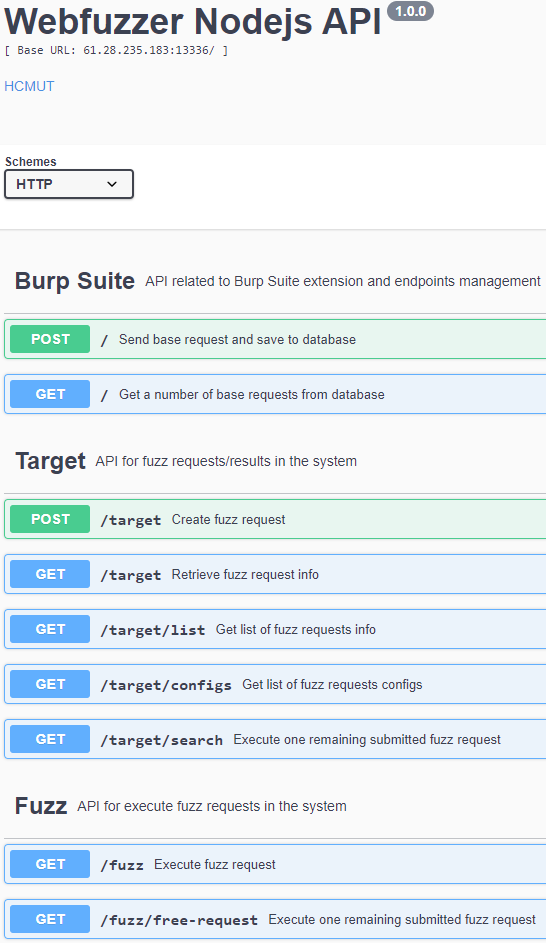
\includegraphics[width=0.5\textwidth,keepaspectratio=true]{images/swagger-api.png}
  \caption{Danh sách các API được cung cấp bởi backend của ứng dụng webfuzzer}
  \label{fig:swagger-api}
\end{figure}
\subsection{Kết nối đến dịch vụ MySQL của hệ điều hành}
\subsection{Mô-đun kiểm thử}
\subsubsection{Mô-đun phân tích request mẫu}
\subsubsection{Mô-đun xây dựng \acrshort{http} request kiểm thử}
\subsubsection{Các mô-đun kiểm thử}
\subsubsection{Mô-đun lưu trữ kết quả kiểm thử}
\section{Giao diện người dùng}
\section{Cơ sở dữ liệu}
Dựa vào thiết kế đã đề ra ở \textbf{Chương 5}, chúng tôi hiện thực cấu trúc cơ sở dữ liệu của ứng dụng webfuzzer gồm ba bảng chính. Bảng \ref{tab:db-tables} dưới đây mô tả tên và chức năng của từng bảng trong lược đồ.
\begin{table}[ht]
    \centering
    \caption{Các bảng trong lược đồ quan hệ}
    \label{tab:db-tables}
    \begin{tabular}[ht]{lll}
        \toprule[1pt]\midrule[0.3pt]
            \textbf{Tên}& &\textbf{Mô tả}\\ 
        \midrule
            Endpoint& &Bảng Endpoint lưu lại các request mẫu mục tiêu được gửi đến máy chủ \\
            {}& &từ phần mở rộng Burp Suite\\
            \addlinespace
            Request& &Bảng Request lưu những yêu cầu kiểm thử một request mẫu \\
            {}& &trong bảng Endpoint của người dùng\\
            \addlinespace
            Result& &Bảng Result lưu kết quả kiểm thử chi tiết \\
            {}& &ứng với mỗi yêu cầu kiểm thử trong bảng Request\\
            \addlinespace
        \midrule[0.3pt]\bottomrule[1pt]
    \end{tabular}
\end{table}
\FloatBarrier
Hình \ref{fig:db-schema} dưới đây mô tả quan hệ giữa các bảng trong lược đồ.
\begin{figure}[H]
  \centering
    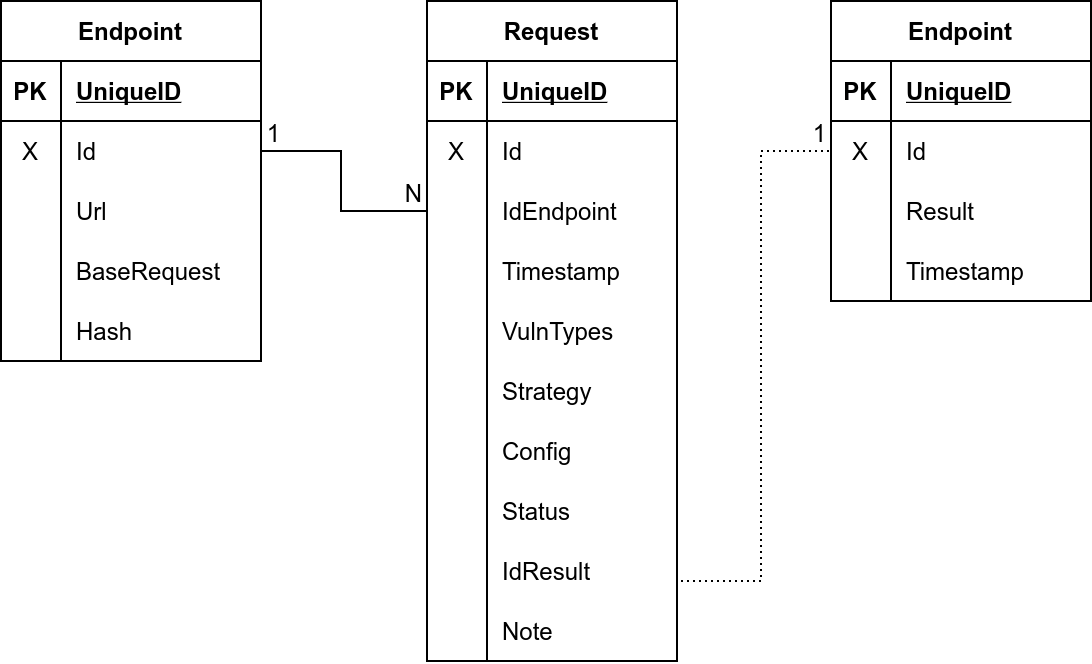
\includegraphics[width=0.75\textwidth,keepaspectratio=true]{images/database-design.png}
  \caption{Sơ đồ mối quan hệ giữa các bảng trong lược đồ}
  \label{fig:db-schema}
\end{figure}
Bảng \texttt{Endpoint} lưu trữ \acrshort{http} request mẫu được gửi từ phần mở rộng Burp Suite đến backend thông qua API \colorbox{gray!30}{\texttt{POST /}}. Request mẫu đó chứa dưới dạng chuỗi dữ liệu JSON trong trường \texttt{BaseRequest}. Trường \texttt{Url} chứa riêng \acrshort{url} của điểm cuối ứng dụng web mục tiêu để thuận lợi trong việc lọc ra những yêu cầu kiểm thử của cùng một trang web thông qua API \colorbox{gray!30}{\texttt{POST /target/search}}. Trường \texttt{Hash} chứa giá trị băm của chuỗi \texttt{BaseRequest}, đảm bảo không lưu hai request mẫu y hệt nhau gây dư thừa dữ liệu. Bảng \texttt{Request} chứa thông tin của các yêu cầu kiểm thử, trong đó trường \texttt{IdEndpoint} là khoá ngoại tham chiếu tới khoá chính \texttt{Id} của bảng \texttt{Endpoint} và trường \texttt{IdResult} là khoá ngoại tham chiếu tới khoá chính \texttt{Id} của bảng \texttt{Result} chứa kết quả kiểm thử (trong trường hợp có lỗ hổng). Mỗi bản ghi trong bảng \texttt{Request} chứa \acrshort{http} request mẫu gửi đến các điểm cuối của ứng dụng web mục tiêu, tập các lỗ hổng cần kiểm thử, trạng thái, và kết quả kiểm thử tương ứng, bao gồm danh sách lỗ hổng của điểm cuối đó và các payload phát hiện được. Trường \texttt{BaseRequest} của bảng \texttt{Endpoint}, trường \texttt{VulnTypes} của bảng \texttt{Request} và \texttt{Result} của bảng \texttt{Result} là các trường có kiểu chuỗi, chứa các giá trị kiểu đối tượng JSON đã được chuỗi hóa như đã đề cập trong phần thiết kế kiến trúc cơ sở dữ liệu ở trên.
% \section{Phần mở rộng trên Burp Suite}
Như đã giới thiệu ở \textbf{Chương 4}, Burp Suite là một khung thức kiểm thử thâm nhập ứng dụng web được viết trên nền Java. Nó không chỉ nổi tiếng và hữu dụng ở những tính năng cơ bản sẵn có như proxy trung gian, bộ lặp lại (repeater) và tuần tự hóa (sequencer) các request, mà còn ở các phần mở rộng của nó. Burp Suite cho phép và hỗ trợ người dùng tự viết các phần mở rộng (extender) bằng ngôn ngữ Java, Python hoặc Ruby để tiện lợi hóa quá trình sử dụng công cụ này cũng như để phát triển thêm các tính năng có sẵn theo mục đích người dùng. Các phần mở rộng này có thể được công khai trên \textbf{BApp Store} của Burp Suite và được sử dụng như một công cụ độc lập trên nền các tính năng cơ bản của nó. Trong phạm vi luận văn này, chúng tôi sử dụng tính năng proxy trung gian, thâm nhập (intruder) để tạo ra request mẫu và hiện thực một phần mở rộng để gửi \acrshort{http} request mẫu đó đến công cụ \textbf{webfuzzer}.\par
Các đối tượng kiểm thử (\acrshort{http} request mẫu) sẽ được người dùng chọn thông qua trình duyệt web có cài đặt proxy. Bằng việc cài đặt tùy chọn proxy trên trình duyệt và trên Burp Suite về cùng một giá trị IP:port (mặc định là \texttt{127.0.0.1:8080} trên Burp Suite), phần mềm này sẽ bắt được tất cả những request được gửi đi từ phía trình duyệt web người dùng, sau đó cho phép chuyển tiếp (forward), loại bỏ (drop) hoặc chuyển những request mà người dùng muốn kiểm thử đến các mô-đun khác của Burp Suite. Giao diện của mô-đun \textbf{Proxy} trong quá trình bắt request được thể hiện trong Hình \ref{fig:burp-proxy} sau.
\begin{figure}[H]
  \centering
    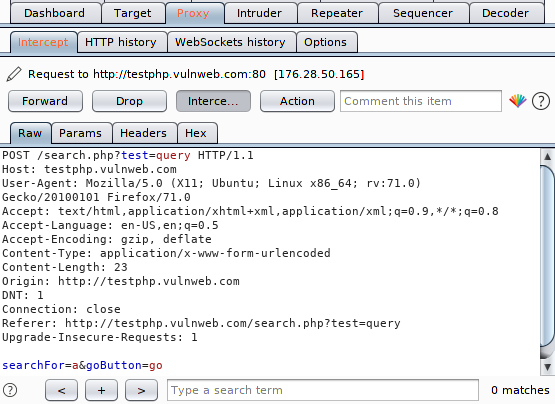
\includegraphics[width=0.75\textwidth,keepaspectratio=true]{images/burp-proxy.png}
  \caption{Sử dụng mô-đun Proxy của Burp Suite để bắt HTTP request}
  \label{fig:burp-proxy}
\end{figure}
Việc tạo request mẫu để gửi cho \textbf{webfuzzer} tiếp tục bằng bước chuyển tiếp request từ \textbf{Proxy} đến mô-đun \textbf{Intruder} để chọn tiếp tham số cần kiểm thử. Mô-đun \textbf{Intruder} chuyên dùng để đánh dấu các vị trí sẽ được thay thế bằng payload bằng cách thêm hoặc bỏ các kí tự ``\texttt{\$}'' bao quanh giá trị của tham số, sau đó chọn chiến lược tấn công (sniper, cluster bomb,...) để gửi đến ứng dụng web mục tiêu. Chúng tôi tận dụng hai mô-đun \textbf{Proxy} và \textbf{Intruder} này để chọn ra đối tượng kiểm thử cho \textbf{webfuzzer}, bao gồm mẫu các tiêu đề \acrshort{http}, đích đến và các tham số cần kiểm thử như Hình \ref{fig:burp-intruder} dưới đây.
\begin{figure}[H]
  \centering
    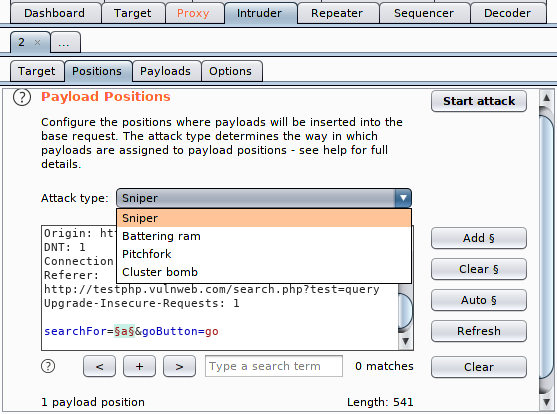
\includegraphics[width=0.75\textwidth,keepaspectratio=true]{images/burp-intruder.png}
  \caption{Giao diện mô-đun Intruder của Burp Suite}
  \label{fig:burp-intruder}
\end{figure}
Sau cùng, chúng tôi hiện thực một phần mở rộng trên Burp Suite để gửi request mẫu đã tạo ra đến công cụ \textbf{webfuzzer}. Burp Suite cung cấp sẵn định dạng các interface cũng như tài liệu Javadoc cần thiết để hiện thực một phần mở rộng như Hình \ref{fig:burp-extender} bên dưới.
\begin{figure}[H]
  \centering
    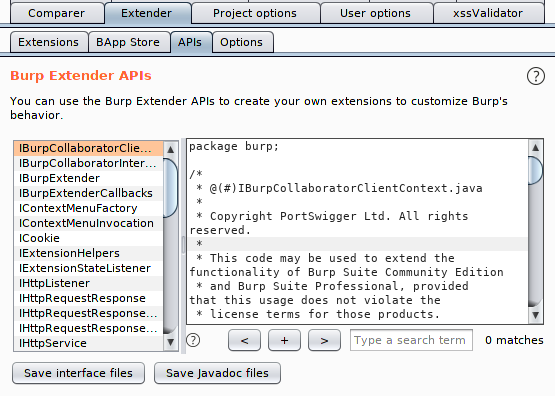
\includegraphics[width=0.75\textwidth,keepaspectratio=true]{images/burp-extender.png}
  \caption{Các phương thức cần để hiện thực một phần mở rộng trên Burp Suite}
  \label{fig:burp-extender}
\end{figure}
Cụ thể, chúng tôi tiến hành xây dựng class \texttt{BurpExtender} bằng cách hiện thực interface \texttt{IBurpExtender} có sẵn, sử dụng ngôn ngữ Java. \textbf{Về giao diện}, phần mở rộng gồm 3 tab chính là ``Configuration'' (chứa textbox nhập địa chỉ IP và port để gửi đến \textbf{webfuzzer}), ``Todo'' và ``About'' dưới dạng các Swing panel trong ngôn ngữ Java. Chúng tôi override lại hàm \texttt{run} của phương thức \texttt{registerExtenderCallbacks} để hiện thực giao diện này.\\
\begin{lstlisting}[language=Java]
@Override
public void run() {
    JPanel jPanel = new JPanel();
    jPanel.setLayout(null);
    JLabel jLabel = new JLabel("Server Address:");
    jLabel.setBounds(10, 10, 500, 30);
    BurpExtender.this.tfServerAdress = new JTextField(BurpExtender.SERVERADRESS);
    BurpExtender.this.tfServerAdress.setBounds(500, 10, 300, 30);
    jPanel.add(jLabel);
    jPanel.add(BurpExtender.this.tfServerAdress);
    JPanel jPanel2 = new JPanel(new GridLayout(2, 1));
    JPanel jPanel3 = new JPanel();
    JLabel jLabel2 = new JLabel("<html><h1>y4t0g4m1 webfuzzer</h1><p>@Author: y4t0g4m1</p><p>@Features:</p></html>");
    jPanel3.add((Component)jLabel2, "Center");
    BurpExtender.this.tabs = new JTabbedPane();
    BurpExtender.this.tabs.add("Configuration", jPanel);
    BurpExtender.this.tabs.add("Todo", jPanel2);
    BurpExtender.this.tabs.add("About", jPanel3);
    BurpExtender.this.mainPanel = new JPanel(new GridLayout(1, 1));
    BurpExtender.this.mainPanel.add(BurpExtender.this.tabs);
    BurpExtender.this.callbacks.customizeUiComponent(
        (Component)BurpExtender.this.tabs);
    BurpExtender.this.callbacks.customizeUiComponent(
        (Component)BurpExtender.this.mainPanel);
    BurpExtender.this.callbacks.addSuiteTab((ITab)BurpExtender.this);
}
\end{lstlisting}
\textbf{Về chức năng}, phần mở rộng này nhận dữ liệu đầu vào là thông tin địa chỉ IP và port của máy chủ công cụ \textbf{webfuzzer}, và nội dung của request mẫu từ mô đun \textbf{Intruder} được hệ thống lại dưới định dạng JSON như sau.\\
\begin{lstlisting}[language=json,firstnumber=1]
"burp":{ 
    "request":"UE9TVCAvc2VhcmNoLnBocD90Z...VhcmNoRm9yPadhpyZnb0J1dHRvbj1nbw==",
    "content_type":"CONTENT_TYPE_URL_ENCODED",
    "body_offset":"516",
    "method":"POST",
    "url":"http://testphp.vulnweb.com:80/search.php?test=query",
    "headers":{ 
        "User-Agent":"Mozilla/5.0 (X11; Ubuntu; Linux x86_64; rv:71.0) Gecko/20100101 Firefox/71.0",
        "Accept":"text/html,application/xhtml+xml,application/xml;q=0.9,*/*;q=0.8",
        "Accept-Language":"en-US,en;q=0.5",
        "Accept-Encoding":"gzip, deflate",
        "Content-Type":"application/x-www-form-urlencoded",
        "Origin":"http://testphp.vulnweb.com",
        "DNT":"1",
        "Connection":"close",
        "Referer":"http://testphp.vulnweb.com/search.php?test=query",
        "Upgrade-Insecure-Requests":"1"
    }
}
\end{lstlisting}
Trường \texttt{request} chứa toàn bộ nội dung của request mẫu dưới dạng base64, các trường còn lại được trích xuất ra bằng các phương thức \texttt{getMethod()}, \texttt{getUrl()}, \texttt{getBodyOffset()}, \texttt{getContentType()}, \texttt{getHeaders()} của class \texttt{IRequestInfo}. Sau đó phần mở rộng tiến hành trích xuất phần thân (body) của request dựa vào giá trị \texttt{body\_offset} thành trường \texttt{data} chứa từng cặp tên tham số - giá trị tương ứng của request. Tiếp theo, nó xây dựng một \acrshort{http} request để gửi request mẫu này tới \textbf{webfuzzer} dưới dạng chuỗi có định dạng JSON được chứa trong phần body của request bằng phương thức \texttt{makeRequest} sau. Địa chỉ IP và port của công cụ được lấy từ textbox ở giao diện và lưu trong biến \texttt{uRL} của class \texttt{BurpExtender} đang hiện thực.\\
\begin{lstlisting}[language=Java]
public IHttpRequestResponse makeRequest(URL uRL, String string) {
    try {
        ArrayList<String> arrayList = new ArrayList<String>();
        arrayList.add("POST / HTTP/1.1");
        arrayList.add("Host: " + uRL.getHost() + ":" + uRL.getPort());
        arrayList.add("User-Agent: BURP18/xnnx");
        arrayList.add("Content-Type: application/json");
        arrayList.add("Connection: close");
        byte[] arrby = this.helpers.stringToBytes(string);
        byte[] arrby2 = this.helpers.buildHttpMessage(arrayList, arrby);
        IHttpRequestResponse iHttpRequestResponse = this.callbacks.makeHttpRequest(this.helpers.buildHttpService(
            uRL.getHost(), uRL.getPort(), uRL.getProtocol() == "https"), arrby2);
        return iHttpRequestResponse;
    }
    catch (Exception exception) {
        this.stdout.println("[!] Loi khi build request toi server: " + exception.getMessage());
        return null;
    }
}
\end{lstlisting}
Kết quả hiện thực của phần mở rộng này là cho phép gửi \acrshort{http} request mẫu từ mô-đun \textbf{Intruder} đến công cụ \textbf{webfuzzer} đã được format lại theo định dạng JSON dưới đây.\\
\begin{lstlisting}[language=json,firstnumber=1]
"python":{ 
    "url":"http://testphp.vulnweb.com:80/search.php?test=query",
    "cookies":"",
    "headers":{ 
        "User-Agent":"Mozilla/5.0 (X11; Ubuntu; Linux x86_64; rv:71.0) Gecko/20100101 Firefox/71.0",
        "Accept":"text/html,application/xhtml+xml,application/xml;q=0.9,*/*;q=0.8",
        "Accept-Language":"en-US,en;q=0.5",
        "Accept-Encoding":"gzip, deflate",
        "Content-Type":"application/x-www-form-urlencoded",
        "Origin":"http://testphp.vulnweb.com",
        "DNT":"1",
        "Connection":"close",
        "Referer":"http://testphp.vulnweb.com/search.php?test=query",
        "Upgrade-Insecure-Requests":"1"
    },
    "data":{ 
        "searchFor":"\xa7a\xa7",
        "goButton":"go"
    },
    "method":"post"
}
\end{lstlisting}
Định dạng JSON trên cũng là cấu trúc thống nhất của một request mẫu trong suốt quá trình kiểm thử và lưu lại nhật kí hoạt động của \textbf{webfuzzer}. Định dạng trên đã được thay đổi một vài lần trong quá trình hiện thực công cụ. Ban đầu chúng tôi sử dụng định dạng JSON nguyên bản như dữ liệu đầu vào của phần mở rộng. Việc này dẫn tới một số khó khăn trong việc chuyển đổi qua lại giữa base64 và chuỗi kí tự thường, tính toán vị trí chèn payload dựa vào trong trường hợp có nhiều hơn một vị trí cần chèn payload, đồng thời cũng gặp khó khăn trong việc lưu lại nhật kí hoạt động một cách minh bạch, dễ kiểm tra lại. Vì những lý do đó, chúng tôi quyết định xây dựng lại request mẫu thành một định dạng thống nhất, tiện lợi hơn để công cụ \textbf{webfuzzer} kiểm thử và ghi nhật kí hoạt động cũng như cho người dùng dễ dàng kiểm tra. Chuỗi ``\texttt{\textbackslash xa7}'' trong trường \texttt{data.searchFor} biểu thị kí tự ``\$'' trong request mẫu. Các kí tự này thường nằm ở trường \texttt{data} hoặc \texttt{url} trong đoạn dữ liệu JSON để đánh dấu những vị trí chèn payload để công cụ xử lí. Hiện tại, sử dụng các mô-đun có sẵn của Burp Suite là phương pháp mạnh mẽ, hiệu quả, trực quan, dễ sử dụng và cá nhân hóa nhất hiện nay để chọn ra \acrshort{http} request cần kiểm thử, so với việc sử dụng các khung thức kiểm thử cũ trên thị trường như BeEF hay Metasploit. 

\section{Máy chủ}

\subsection{Mô-đun xây dựng HTTP request}
Mô-đun này nhận vào request mẫu chứa đầy đủ thông tin và các vị trí cần chèn payload từ mô-đun socket listener ở trên. Đầu tiên mô-đun này sẽ tạo ra thêm các request mẫu dựa trên request mẫu nhận được sao cho trong một request chỉ chứ một vị trí chèn payload. Giả sử trường \texttt{data} trong request mẫu có giá trị như sau.\\
\begin{lstlisting}[language=json,firstnumber=1]
"data":{ 
    "searchFor":"\xa7a\xa7",
    "goButton":"\xa7go\xa7"
}
\end{lstlisting}
Lúc này có hai chỗ cần chèn payload vào, đó là giá trị của trường \texttt{searchFor} và \texttt{goButton}. Trước khi tiến hành chèn payload, mô-đun này sẽ tách request mẫu thành hai request mẫu riêng, mỗi request chứa một vị trí chèn payload. Sau đó mới lần lượt chèn các payload cần kiểm thử vào từng request để dựng thành một HTTP request hoàn chỉnh. Chiến lược này tương đương với chiến lược \texttt{sniper} của mô-đun \textbf{Intruder} của Burp Suite. Đoạn mã Python dưới đây hiện thực quá trình chèn payload và thiết kế hàng đợi của mô-đun này.\\
\begin{python}
def prepareRequest(request, _cfg):
    global queue
    global cfg

    queue = Queue()
    cfg = {}

    fileToFuzz = _cfg["fileToFuzz"]
    respNormal = buildNormalRequest(request)
    parseRequest = ParseRequest(request)
    indexFound = parseRequest.getPatternFromRequest()
    requestList = parseRequest.appendPayloadToRequest(indexFound, fileToFuzz)
    queue = list_to_queue(requestList, queue)

    cfg = {"queue": queue, "respNormal": respNormal, "config":_cfg}

    print(yellow + "Start checking for vulnerabilities...." + end)
    threads = [gevent.spawn(preFuzzing, cfg) for i in range(2)] 
    try:
        gevent.joinall(threads)
    except KeyboardInterrupt as e:
        print(e)
        pass
    print(blue + "Done " + _cfg["label"] + " fuzzing" + end)
\end{python}
Ban đầu chúng tôi gặp rất nhiều khó khăn trong việc lần lượt kiểm thử từng payload đối với một lỗ hổng bảo mật. Lý do vì \acrshort{http} là một giao thức không trạng thái (stateless), một HTTP response trả về tương ứng với duy nhất môt HTTP request trước đó gửi đến ứng dụng web. Trong trường hợp chúng tôi muốn hiện thực được công cụ \texttt{webfuzzer}, điều kiện tiên quyết là phải tuần tự hóa được quá trình kiểm thử trên một danh sách các payload. Điều này có nghĩa là sau khi công cụ gửi request chứa payload 1, phải nhận về response tương ứng thành công mới trước khi gửi tiếp request chứa payload 2, nếu không tuân thủ trình tự trên thì công cụ sẽ không xác định được payload nào gây ra lỗi để ghi lại kết quả kiểm thử. Để giải quyết vấn đề trên, chúng tôi đề xuất hiện thực một hàng đợi, lần lượt đẩy vào từng request với cấu hình kiểm thử loại lỗ hổng tương ứng, dequeue request hiện tại, gửi đi và nhận về response xong mới dequeue request tiếp theo để xử lí. Cấu hình kiểm thử cụ thể sẽ được trình bày ở \textbf{Phần 5.6.1}. Chúng tôi đã sử dụng thư viện \texttt{gevent} của Python để hiện thực hàng đợi này. \texttt{Gevent} là một thư viện gọn nhẹ, hỗ trợ đồng bộ hóa các thao tác giao tiếp với mạng internet nói chung và các ứng dụng web nói riêng dựa trên các trình cộng hành (coroutine-based). Thư viện này cho phép tuần tự hóa quá trình xử lí một hàng đợi các request bằng cách định ra những \textit{đối tượng Greenlet}, các đối tượng này được khai báo kèm theo một hàm thực thi, chỉ khi thực thi xong hàm đó với một đối tượng thì mới được thực thi hàm đó với đối tượng tiếp theo trong hàng đợi. Áp dụng vào công cụ, mỗi request hoàn chỉnh sau khi dựng lên cùng với payload lúc này được đính kèm với hàm \texttt{preFuzzing} và cấu hình tương ứng bằng câu lệnh \\\texttt{threads = [gevent.spawn(preFuzzing, cfg) for i in range(2)]} trong đoạn mã trên. Điều này cho phép mỗi payload cùng với cấu hình tương ứng lần lượt được đưa vào hàm \texttt{preFuzzing} theo thứ tự như chúng tôi mong muốn.

\section{Bộ hậu xử lí và lưu trữ}
Bộ phận này đảm nhiệm việc nhận biết lỗ hổng bảo mật trên ứng dụng web thông qua \acrshort{http} response trả về, đồng thời hiện thực hệ thống quản lý nhật kí hoạt động, ghi lại nhật kí một cách tách bạch, có hệ thống đối với từng request mẫu và từng loại lỗ hổng bảo mật khác nhau.
\subsection{Mô-đun xác nhận lỗi trên HTTP response}
Mô-đun này đảm nhiệm việc xử lí HTTP response trả về từ ứng dụng web và dựa vào response đó để phát hiện lỗ hổng bảo mật. Chúng tôi sử dụng thư viện \texttt{requests} của Python để xử lí \acrshort{http} response trong suốt quá trình tương tác với ứng dụng web mục tiêu. Các response mà mô-đun này nhận được đều thuộc class \texttt{requests.Response}, chúng tôi sử dụng những một số thuộc tính của class này để phục vụ quá trình xử lí kêt quả kiểm thử.
\begin{itemize}
    \item \textbf{status\_code} chứa mã trạng thái của các response trả về.
    \item \textbf{headers} chứa các tiêu đề HTTP của response.
    \item \textbf{text} chứa nội dung unicode của response, có kiểu tùy vào trường \texttt{Content-Type} trên tiêu đề.
    \item \textbf{elapsed} chứa thời gian xử lí request tính theo giây, từ lúc gửi request đến khi nhận được response tương ứng.
\end{itemize}

Kết hợp các cấu hình này và các thuộc tính của biến response trả về, chúng tối định ra chi tiết phương thức phát hiện các lỗ hổng bảo mật như sau.

\subsubsection{Đối với lỗ hổng \acrlong{lfi}}
Để phát hiện lỗ hổng \acrshort{lfi}, chúng tôi thực hiện tương tụ như việc so trùng trong trường hợp \texttt{Content-Type} của response trả về không phải là mã \acrshort{html} đối với lỗ hổng \acrshort{xss}. Cụ thể, chúng tôi cố gắng đọc nội dung tập tin \texttt{/etc/passwd} bằng các payload được chèn vào, tập tin này luôn bắt đầu bằng chuỗi ``\texttt{root:x:}'' trên các máy chủ ứng dụng web nhân Unix. Một khi response trả về có chuỗi này thì khả năng rất cao ứng dụng web mắc phải lỗ hổng \acrshort{lfi}.\par
Tuy nhiên cũng có khả năng các payload này đọc được một tập tin \texttt{/etc/passwd} giả trong quá trình kiểm thử. Ứng dụng web có thể thêm vào thư mục lưu trữ trang web một đường dẫn đến tập tin \texttt{/etc/passwd} có chứa chuỗi ``\texttt{root:x:}'' trong nội dung. Để khắc phục nhược điểm đó, trong tương lai chúng tôi sẽ thiết kế thêm các cấu hình cũng như payload để đọc thêm nhiều tập tin thông tin hệ thống trên Unix khác như \texttt{/etc/issue}, \texttt{/etc/passwd}, \texttt{/etc/shadow}, \texttt{/etc/group}, \texttt{/etc/hosts}, \texttt{/etc/motd}, \texttt{/etc/mysql/my.cnf}, \texttt{/proc/self/environ}, \texttt{/proc/version}, \texttt{/proc/cmdline},... sau khi đã \texttt{[passed]} được tập tin \texttt{/etc/passwd}. Điều này sẽ giúp giảm tỉ lệ dương tính giả của phương pháp phát hiện này. Đồng thời chúng tôi cũng sẽ mở rộng phạm vi phát hiện trên các ứng dụng web chạy trên hệ điều hành Windows Server bằng các payload đọc các tập tin thông tin hệ thống trên Windows như \texttt{boot.ini}, \texttt{windows/win.ini}, \texttt{winnt/win.ini},... Hiện tại do giới hạn thời gian và nguồn lực mà chúng tôi chưa thể triệt tiêu hoàn toàn tỉ lệ dương tính giả trong việc phát hiện lỗ hổng bảo mật này.

\subsubsection{Đối với lỗ hổng time-based \acrlong{sqli}}
Để phát hiện lỗ hổng này, chúng tôi dựa vào thuộc tính \texttt{elapsed} chứa thời gian xử lí request của ứng dụng web và thuộc tính \texttt{time} trong thiết lập cấu hình để loại bỏ những request được xử lí quá nhanh. Các payload kiểm thử lỗ hổng này đều dùng hàm hoãn thời gian 10 giây (\texttt{SLEEP(10), PG\_SLEEP(10), WAITFOR DELAY '0:0:10', WAITFOR TIME '0:0:10'}) kết hợp với việc sử dụng hàm benchmark trả về tổng thời gian thực thi lệnh \texttt{MD5('Y4T0G4M11337')} 1000000 lần cộng với các cách thức đóng ngoặc, chú thích để tránh gặp lỗi cú pháp trong quá trình thực thi câu lệnh SQL chứa payload ở phía máy chủ. Về mặt lý thuyết, nếu ứng dụng web mắc lỗi này thì thời gian xử lí một request chứa các payload kiểm thử không thể ít hơn 10 giây được. Về mặt thực tế, khi kiểm thử một số trang web bằng \textbf{webfuzzer} thì thời gian xử lí các request chứa payload này dao động từ 20 giây đến 60 giây. Đó là lý do chúng tôi đặt thời gian tối đa cho một request kiểm thử là 70 giây, nếu thời gian thực hiện quá 70 giây thì chúng tôi đánh dấu payload tương ứng là \texttt{[skeptical]} vì vẫn có trường hợp thời gian xử lí lâu hơn 60 giây ở các máy chủ web cấu hình thấp hơn. Câu lệnh dưới đây có chức năng tạo, gửi request kèm cài đặt thời gian timed-out là 70 giây và nhận về một giá trị thuộc class \texttt{requests.Response} gán vào biến \texttt{resp}.\\
\begin{python}
resp = request(self.method, self.url, cookies=self.cookies, headers=self.headers, data=self.data, timeout=70)
\end{python}
Đoạn mã Python dưới đây hiện thực quá trình phát hiện lỗ hổng time-based \acrshort{sqli} theo cấu hình và phương pháp đã định trước. Biến \texttt{isTimedOut} có giá trị là \texttt{True} khi đã có ngoại lệ về thời gian xảy ra trong quá trình thực hiện request. Nếu bị timed-out trong lúc kiểm thử lỗ hổng time-based \acrshort{sqli} (\texttt{config['id'] == 3}) thì chúng tôi đánh dấu payload hiện tại là \texttt{[skeptical]}. Còn lại trong trường hợp request được xử lí bình thường thì miễn thời gian trả về response từ ứng dụng web lớn hơn thời gian được thiết lập trong thuộc tính \texttt{time} của cấu hình thì chắc chắn ứng dụng web có lỗ hổng này. Tỉ lệ dương tính giả đối với các trường hợp kiểm thử đã \texttt{[passed]} là bằng 0.\\
\begin{python}
def timebasedDetect(req, resp, payload, isTimedOut, config, method=None):
    if isTimedOut:
        if config['id'] == 3:
            print(purple + "[skeptical]    " + yellow + payload + "\t" + end)
            addToLog(req, config['label'], "SKEPTICAL: " + unescapePayload(payload), method, config["output"])
    else:
        print(red + "[failed]    " + yellow + payload + "\t" +  end)
    elif int(resp.elapsed.total_seconds()) > config['time']:
        print(green + "[passed]    " + yellow + str(resp.status_code) + "\t" + str(len(resp.text)) + "\t" + "{:<10}".format(str(resp.elapsed.total_seconds())) + "\t" +  payload + "\t"+ end)
        addToLog(req, config['label'], unescapePayload(payload), method, config["output"])
    else:
        print(red + "[failed]    " + yellow + str(resp.status_code) + "\t" + str(len(resp.text)) + "\t" + "{:<10}".format(str(resp.elapsed.total_seconds())) + "\t" +  payload + "\t" +  end)
\end{python}

\chapter{Kiểm định và đánh giá kết quả}
Chương này chúng tôi trình bày kết quả sử dụng ứng dụng webfuzzer để kiểm thử một số ứng dụng web và so sánh trực tiếp với quá trình kiểm thử bằng chức năng \texttt{Intruder} của công cụ Burp Suite để đánh giá kết quả đạt được thông qua quá trình thiêt kế và hiện thực ứng dụng.
\section{Thiết lập kiểm thử ở Burp Suite}
Ở ứng dụng Burp Suite, chúng tôi cần thiết lập thời gian timeout của các \acrshort{http} request kiểm thử, danh sách payload và các chuỗi, biểu thức chính quy so trùng trên response. Các thông số trên lần lượt tương ứng với các trường \texttt{time}, \texttt{payloadFile} và \texttt{match, matchFile, regex} trong cấu hình kiểm thử. Chức năng \texttt{Intruder} không cho phép điều chỉnh timeout riêng của các request trong chức năng này, chúng tôi phải thiết lập thời gian timeout toàn cục cho một dự án (project) của Burp Suite dưới dạng đối tượng JSON như Đoạn mã \ref{lst:setup-timeout-burp} sau, đơn vị tính là mili giây. Đây cũng là một sự tiện lợi khi sử dụng webfuzzer vì người dùng có thể dễ dàng điều chỉnh thông số này ở cấu hình kiểm thử tùy theo từng loại lỗ hổng.
\begin{lstlisting}[style=ES6, label={lst:setup-timeout-burp}, caption={Thiết lập thời gian timeout của request kiểm thử ở Burp Suite}]
"timeouts":{
    "domain_name_resolution_timeout":300000,
    "failed_domain_name_resolution_timeout":60000,
    "normal_timeout":10000,
    "open_ended_response_timeout":10000
},
\end{lstlisting}
Các chuỗi và biểu thức chính quy so trùng có thể được thêm vào bằng tay ở mục \texttt{Grep - Match} trong tab \texttt{Options} như Hình \ref{fig:setup-grep-string-regex} sau.
\begin{figure}[H]
    \centering
        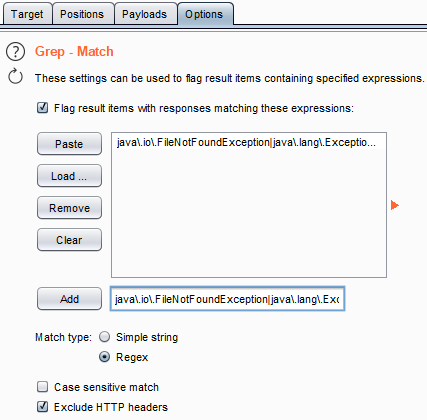
\includegraphics[width=0.6\textwidth,keepaspectratio=true]{images/setup-grep-string-regex.png}
    \caption{Thêm thiết lập so trùng vào cấu hình kiểm thử ở Burp Suite}
    \label{fig:setup-grep-string-regex}
\end{figure}
Tương tự, chức năng danh sách payload có thể được thêm vào tuần tự hoặc trích xuất từ tập tin ở mục \texttt{Payload Options [Simple list]} trong tab \texttt{Payloads} như Hình \ref{fig:setup-payload-list} sau. Việc lưu trữ và sao chép các thiết lập kiểm thử (payload, các chuỗi so trùng) giữa các đối tượng kiểm thử trong chức năng \texttt{Intruder} khá phiền phức so với webfuzzer. Người dùng webfuzzer chỉ việc chọn những cấu hình kiểm thử thường dùng đã được định nghĩa sẵn ở backend, đây cũng là một ưu điểm của ứng dụng so với Burp Suite.
\begin{figure}[H]
    \centering
        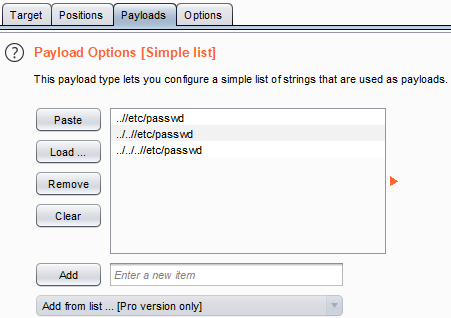
\includegraphics[width=0.6\textwidth,keepaspectratio=true]{images/setup-payload-list.png}
    \caption{Thêm payload vào cấu hình kiểm thử ở Burp Suite}
    \label{fig:setup-payload-list}
\end{figure}
Trong quá trình kiểm thử bằng Burp Suite, chúng tôi phải tự nhận diện lỗ hổng thủ công thông qua giao diện kiểm thử của chức năng \texttt{Intruder} như Hình \ref{fig:fuzzing-burp} sau.
\begin{figure}[H]
    \centering
        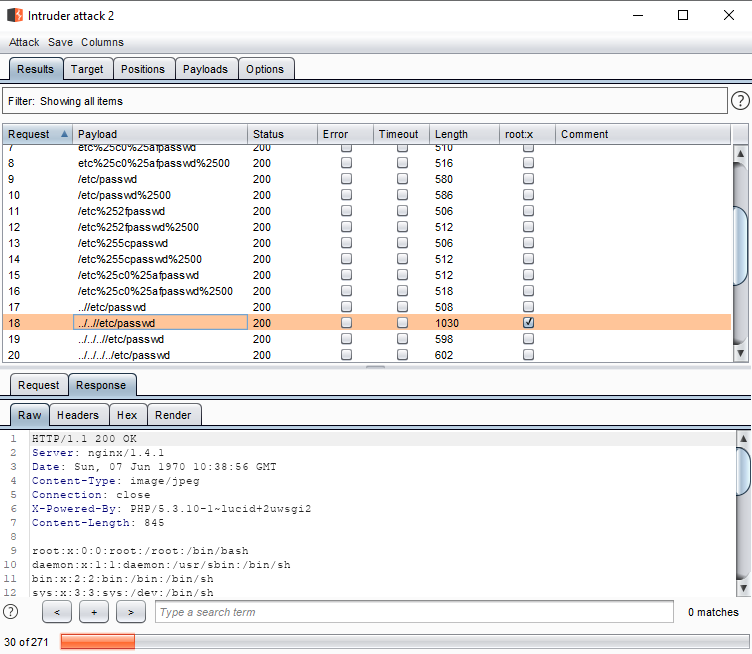
\includegraphics[width=\textwidth,keepaspectratio=true]{images/fuzzing-burp.png}
    \caption{Giao diện kiểm thử bằng chức năng \texttt{Intruder} của Burp Suite}
    \label{fig:fuzzing-burp}
\end{figure}
Từng request kiểm thử chứa payload tương ứng sẽ được hiển thị thành một dòng trên giao diện, lần lượt thể hiện các thông tin của request đó, backend của webfuzzer cũng xuất ra kết quả kiểm thử tương tự trên terminal. Các chuỗi và biểu thức chính quy so trùng được hiển thị dưới dạng một cột, cột này sẽ được đánh dấu khi nội dung response tương ứng có chứa chuỗi đó như Hình \ref{fig:fuzzing-burp}. Khung bên dưới hiển thị nội dung chi tiết của response ứng với request kiểm thử đang chọn ở trên. Tương tự khi request kiểm thử vượt quá thời gian timeout đã thiết lập thì cột \texttt{Timeout} trên giao diện sẽ được đánh dấu. Sau khi quá trình kiểm thử kết thúc, người dùng phải tự hệ thống lại xem payload nào phát hiện được lỗ hổng.\par
\section{Tập kiểm thử và kết quả đánh giá công cụ}
Để quá trình đánh giá kết quả được khách quan, chúng tôi sử dụng tập kiểm thử gồm có các trang web có và không có các lỗ hổng \acrshort{lfi} và time-based \acrshort{sqli}. Chúng tôi đồng thời kiểm thử các trang web này bằng webfuzzer và Burp Suite, so sánh kết quả kiểm thử, các payload phát hiện lỗ hổng nếu có, và thời gian kiểm thử mỗi mục tiêu của hai phần mềm này. Máy tính thực hiện kiểm thử trên cả hai phần mềm sử dụng CPU Intel Core i5-9400F và 8GB DDR4 RAM, trên hệ điều hành Ubuntu 20.04 LTS Focal. Ở chức năng \texttt{Intruder} của Burp Suite chúng tôi thiết lập số lượng luồng (threads) là 1, số lần thử gửi lại request khi thất bại là 0, và không áp dụng các phương pháp encode nào khác trên payload vì trong webfuzzer chúng tôi không hiện thực các chức năng này. Trong quá trình trình bày kết quả đánh giá, chúng tôi rút gọn trường cookies và headers của các đối tượng kiểm thử (request mẫu) trong trường hợp không cần thiết. Chúng tôi ghi lại kết quả đánh giá dưới dạng Bảng \ref{tab:sample-testing-results} sau, trong đó \texttt{N} là số payload phát hiện lỗi (trong số 271 payload \acrshort{lfi} và 476 payload time-based \acrshort{sqli}) và \texttt{T} là thời gian kiểm thử của ứng dụng tính bằng mili giây.
\FloatBarrier
\begin{table}[ht]
    \centering
    \caption{Mẫu bảng so sánh kết quả kiểm thử ứng dụng webfuzzer so với Burp Suite}
    \label{tab:sample-testing-results}
    \begin{tabular}[ht]{ccccc}
        \toprule[1pt]\midrule[0.3pt]
            \multirow{2}{*}{\textbf{Loại lỗ hổng}}&\multicolumn{2}{c}{\textbf{Webfuzzer}}&\multicolumn{2}{c}{\textbf{Burp Suite}}\\
            \cmidrule(lr){2-3}\cmidrule(lr){4-5}{}&Số payload&Thời gian&Số payload&Thời gian\\
        \midrule[0.3pt]
            \textbf{\acrshort{lfi}}&N&T&N&T\\\addlinespace
            \textbf{Time-based \acrshort{sqli}}&N&T&N&T\\
        \midrule[0.3pt]\bottomrule[1pt]
    \end{tabular}
\end{table}
\FloatBarrier
Nội dung request mẫu và kết quả kiểm thử các request này trên hai ứng dụng lần lượt được trình bày bằng các Đoạn mã và các Bảng dưới đây.
\begin{lstlisting}[style=ES6, label={lst:base-request-1}, caption={Request mẫu 1 có lỗ hổng \acrshort{lfi}}]
{
    "url": "http://testphp.vulnweb.com:80/showimage.php?file=§./pictures/1.jpg§",
    "cookies": "",
    "headers": { ... },
    "method": "get"
}
\end{lstlisting}
\FloatBarrier
\begin{table}[ht]
    \centering
    \caption{Kết quả kiểm thử request mẫu 1}
    \label{tab:testing-result-1}
    \begin{tabular}[ht]{ccccc}
        \toprule[1pt]\midrule[0.3pt]
            \multirow{2}{*}{\textbf{Loại lỗ hổng}}&\multicolumn{2}{c}{\textbf{Webfuzzer}}&\multicolumn{2}{c}{\textbf{Burp Suite}}\\
            \cmidrule(lr){2-3}\cmidrule(lr){4-5}{}&Số payload&Thời gian&Số payload&Thời gian\\
        \midrule[0.3pt]
            \textbf{\acrshort{lfi}}&1&89998&1&88400\\
        \midrule[0.3pt]\bottomrule[1pt]
    \end{tabular}
\end{table}
\FloatBarrier
\begin{lstlisting}[style=ES6, label={lst:base-request-2}, caption={Request mẫu 2 có lỗ hổng time-based \acrshort{sqli}}]
{
    "url": "http://testphp.vulnweb.com:80/search.php?test=query",
    "cookies": "",
    "headers": { ... },
    "data": {
        "searchFor": "a§§",
        "goButton": "go"
    },
    "method": "post"
}
\end{lstlisting}
\FloatBarrier
\begin{table}[ht]
    \centering
    \caption{Kết quả kiểm thử request mẫu 2}
    \label{tab:testing-result-2}
    \begin{tabular}[ht]{ccccc}
        \toprule[1pt]\midrule[0.3pt]
            \multirow{2}{*}{\textbf{Loại lỗ hổng}}&\multicolumn{2}{c}{\textbf{Webfuzzer}}&\multicolumn{2}{c}{\textbf{Burp Suite}}\\
            \cmidrule(lr){2-3}\cmidrule(lr){4-5}{}&Số payload&Thời gian&Số payload&Thời gian\\
        \midrule[0.3pt]
            \textbf{Time-based \acrshort{sqli}}&14&298195&14&299600\\
        \midrule[0.3pt]\bottomrule[1pt]
    \end{tabular}
\end{table}
\FloatBarrier
\begin{lstlisting}[style=ES6, label={lst:base-request-3}, caption={Request mẫu 3}]
{
    "url": "http://www.daotaonlyt.edu.vn:80/img/§§",
    "cookies": { ... },
    "headers": { ... },
    "method": "get"
}
\end{lstlisting}
\FloatBarrier
\begin{table}[ht]
    \centering
    \caption{Kết quả kiểm thử request mẫu 3}
    \label{tab:testing-result-3}
    \begin{tabular}[ht]{ccccc}
        \toprule[1pt]\midrule[0.3pt]
            \multirow{2}{*}{\textbf{Loại lỗ hổng}}&\multicolumn{2}{c}{\textbf{Webfuzzer}}&\multicolumn{2}{c}{\textbf{Burp Suite}}\\
            \cmidrule(lr){2-3}\cmidrule(lr){4-5}{}&Số payload&Thời gian&Số payload&Thời gian\\
        \midrule[0.3pt]
            \textbf{\acrshort{lfi}}&0&2925&0&3500\\
        \midrule[0.3pt]\bottomrule[1pt]
    \end{tabular}
\end{table}
\FloatBarrier
\begin{lstlisting}[style=ES6, label={lst:base-request-4}, caption={Request mẫu 4 có lỗ hổng time-based \acrshort{sqli}}]
{
    "url": "http://artistclub.vn:80/",
    "cookies": { ... },
    "headers": { ... },
    "data": {
        "email_nhantin": "aaaa@gmail.com§§"
    },
    "method": "post"
}
\end{lstlisting}
\FloatBarrier
\begin{table}[ht]
    \centering
    \caption{Kết quả kiểm thử request mẫu 4}
    \label{tab:testing-result-4}
    \begin{tabular}[ht]{ccccc}
        \toprule[1pt]\midrule[0.3pt]
            \multirow{2}{*}{\textbf{Loại lỗ hổng}}&\multicolumn{2}{c}{\textbf{Webfuzzer}}&\multicolumn{2}{c}{\textbf{Burp Suite}}\\
            \cmidrule(lr){2-3}\cmidrule(lr){4-5}{}&Số payload&Thời gian&Số payload&Thời gian\\
        \midrule[0.3pt]
            \textbf{Time-based \acrshort{sqli}}&7&92952&7&89700\\
        \midrule[0.3pt]\bottomrule[1pt]
    \end{tabular}
\end{table}
\FloatBarrier
\begin{lstlisting}[style=ES6, label={lst:base-request-5}, caption={Request mẫu 5}]
{
    "url": "http://artistclub.vn:80/upload/sanpham/
        §b814bf98-5aad-4146-ade5-6a41f3b631490060_323x360.jpeg§",
    "cookies": { ... },
    "headers": { ... },
    "method": "get"
}
\end{lstlisting}
\FloatBarrier
\begin{table}[ht]
    \centering
    \caption{Kết quả kiểm thử request mẫu 5}
    \label{tab:testing-result-5}
    \begin{tabular}[ht]{ccccc}
        \toprule[1pt]\midrule[0.3pt]
            \multirow{2}{*}{\textbf{Loại lỗ hổng}}&\multicolumn{2}{c}{\textbf{Webfuzzer}}&\multicolumn{2}{c}{\textbf{Burp Suite}}\\
            \cmidrule(lr){2-3}\cmidrule(lr){4-5}{}&Số payload&Thời gian&Số payload&Thời gian\\
        \midrule[0.3pt]
            \textbf{\acrshort{lfi}}&0&4086&0&4900\\
        \midrule[0.3pt]\bottomrule[1pt]
    \end{tabular}
\end{table}
\FloatBarrier
\begin{lstlisting}[style=ES6, label={lst:base-request-6}, caption={Request mẫu 6}]
{
    "url": "http://mwc.com.vn:80/search?s=a§§",
    "cookies": { ... },
    "headers": { ... },
    "method": "get"
}
\end{lstlisting}
\FloatBarrier
\begin{table}[ht]
    \centering
    \caption{Kết quả kiểm thử request mẫu 6}
    \label{tab:testing-result-6}
    \begin{tabular}[ht]{ccccc}
        \toprule[1pt]\midrule[0.3pt]
            \multirow{2}{*}{\textbf{Loại lỗ hổng}}&\multicolumn{2}{c}{\textbf{Webfuzzer}}&\multicolumn{2}{c}{\textbf{Burp Suite}}\\
            \cmidrule(lr){2-3}\cmidrule(lr){4-5}{}&Số payload&Thời gian&Số payload&Thời gian\\
        \midrule[0.3pt]
            \textbf{Time-based \acrshort{sqli}}&0&52760&0&54300\\
        \midrule[0.3pt]\bottomrule[1pt]
    \end{tabular}
\end{table}
\FloatBarrier
\begin{lstlisting}[style=ES6, label={lst:base-request-7}, caption={Request mẫu 7 có lỗ hổng time-based \acrshort{sqli}}]
{
    "url": "http://www.monitoringris.org:80/index.php?id=30§§",
    "cookies": "",
    "headers": { ... },
    "method": "get"
}
\end{lstlisting}
\FloatBarrier
\begin{table}[ht]
    \centering
    \caption{Kết quả kiểm thử request mẫu 7}
    \label{tab:testing-result-7}
    \begin{tabular}[ht]{ccccc}
        \toprule[1pt]\midrule[0.3pt]
            \multirow{2}{*}{\textbf{Loại lỗ hổng}}&\multicolumn{2}{c}{\textbf{Webfuzzer}}&\multicolumn{2}{c}{\textbf{Burp Suite}}\\
            \cmidrule(lr){2-3}\cmidrule(lr){4-5}{}&Số payload&Thời gian&Số payload&Thời gian\\
        \midrule[0.3pt]
            \textbf{Time-based \acrshort{sqli}}&4&434913&4&430200\\
        \midrule[0.3pt]\bottomrule[1pt]
    \end{tabular}
\end{table}
\FloatBarrier
\begin{lstlisting}[style=ES6, label={lst:base-request-8}, caption={Request mẫu 8 có lỗ hổng time-based \acrshort{sqli}}]
{
    "url": "http://www.daotaonlyt.edu.vn:80/index.php?id=320§§",
    "cookies": { ... },
    "headers": { ... },
    "method": "get"
}
\end{lstlisting}
\FloatBarrier
\begin{table}[ht]
    \centering
    \caption{Kết quả kiểm thử request mẫu 8}
    \label{tab:testing-result-8}
    \begin{tabular}[ht]{ccccc}
        \toprule[1pt]\midrule[0.3pt]
            \multirow{2}{*}{\textbf{Loại lỗ hổng}}&\multicolumn{2}{c}{\textbf{Webfuzzer}}&\multicolumn{2}{c}{\textbf{Burp Suite}}\\
            \cmidrule(lr){2-3}\cmidrule(lr){4-5}{}&Số payload&Thời gian&Số payload&Thời gian\\
        \midrule[0.3pt]
            \textbf{Time-based \acrshort{sqli}}&4&66493&4&64900\\
        \midrule[0.3pt]\bottomrule[1pt]
    \end{tabular}
\end{table}
\FloatBarrier
\begin{lstlisting}[style=ES6, label={lst:base-request-9}, caption={Request mẫu 9 có lỗ hổng time-based \acrshort{sqli}}]
{
    "url": "http://csdl.vietnamtourism.gov.vn:80/index.php/
        search/?data=cslt&title=a§§",
    "cookies": "",
    "headers": { ... },
    "method": "get"
}
\end{lstlisting}
\FloatBarrier
\begin{table}[ht]
    \centering
    \caption{Kết quả kiểm thử request mẫu 9}
    \label{tab:testing-result-9}
    \begin{tabular}[ht]{ccccc}
        \toprule[1pt]\midrule[0.3pt]
            \multirow{2}{*}{\textbf{Loại lỗ hổng}}&\multicolumn{2}{c}{\textbf{Webfuzzer}}&\multicolumn{2}{c}{\textbf{Burp Suite}}\\
            \cmidrule(lr){2-3}\cmidrule(lr){4-5}{}&Số payload&Thời gian&Số payload&Thời gian\\
        \midrule[0.3pt]
            \textbf{Time-based \acrshort{sqli}}&86&1572156&86&1481300\\
        \midrule[0.3pt]\bottomrule[1pt]
    \end{tabular}
\end{table}
\FloatBarrier
\begin{lstlisting}[style=ES6, label={lst:base-request-10}, caption={Request mẫu 10 có lỗ hổng time-based \acrshort{sqli}}]
{
    "url": "http://www.hanglahangdoc.com:80/tim_kiem.aspx?keyword=a§§",
    "cookies": { ... },
    "headers": { ... },
    "method": "get"
}
\end{lstlisting}
\FloatBarrier
\begin{table}[ht]
    \centering
    \caption{Kết quả kiểm thử request mẫu 10}
    \label{tab:testing-result-10}
    \begin{tabular}[ht]{ccccc}
        \toprule[1pt]\midrule[0.3pt]
            \multirow{2}{*}{\textbf{Loại lỗ hổng}}&\multicolumn{2}{c}{\textbf{Webfuzzer}}&\multicolumn{2}{c}{\textbf{Burp Suite}}\\
            \cmidrule(lr){2-3}\cmidrule(lr){4-5}{}&Số payload&Thời gian&Số payload&Thời gian\\
        \midrule[0.3pt]
            \textbf{Time-based \acrshort{sqli}}&6&219560&6&212800\\
        \midrule[0.3pt]\bottomrule[1pt]
    \end{tabular}
\end{table}
\FloatBarrier
Qua quá trình kiểm thử các request mẫu trên, chúng tôi nhận thấy các payload phát hiện lỗi ở cả hai ứng dụng đều giống hệt nhau, đây là thành công lớn nhất trong quá trình hiện thực webfuzzer, ứng dụng này đã mô phỏng thành công một phần chức năng \texttt{Intruder} của Burp Suite như hướng phát triển công cụ đã đề ra ở \textbf{Chương 4}. Thời gian kiểm thử của webfuzzer cũng xấp xỉ Burp Suite, chỉ chậm hơn khoảng 2-10 giây tùy vào mỗi request mẫu, hơn nữa webfuzzer có phần nhanh hơn Burp Suite ở các request mẫu mà cả hai ứng dụng đều không phát hiện được lỗ hổng. Vì vậy ngoài lý do không thể tránh khỏi về kết nối, đường truyền giữa các lần kiểm thử, chúng tôi nhận định khoảng thời gian chênh lệch trong việc kiểm thử các request mẫu có lỗ hổng phần lớn đến từ việc lưu trữ kết quả kiểm thử vào cơ sở dữ liệu, do đó chênh lệch thời gian vài giây là một khoản đánh đổi chấp nhận được. Thời gian phản hồi của các \acrshort{http} request gửi đến backend webfuzzer được triển khai ở máy chủ nội bộ (\href{http://localhost:13336/}{\texttt{http://localhost:13336/}}) hoặc ở \acrshort{vps} (\href{http://61.28.235.183:13336/}{\texttt{http://61.28.235.183:13336/}}) chỉ dao động trong khoảng 20-200 mili giây.\par
Xét về trải nghiệm người dùng, ứng dụng webfuzzer trực quan và tiện lợi hơn Burp Suite rất nhiều. Thay vì việc thiết lập cấu hình kiểm thử và nhận diện lỗ hổng thủ công ở Burp Suite như đã mô tả ở \textbf{Đề mục 7.1}, webfuzzer đã tích hợp sẵn khả năng nhận diện lỗ hổng trong mô-đun kiểm thử, đồng thời tổng hợp sẵn những cấu hình kiểm thử tiện dụng, dễ dàng chỉnh sửa. Người dùng chỉ việc chọn request mẫu và loại lỗ hổng, kết quả kiểm thử sẽ được ứng dụng webfuzzer cung cấp chi tiết, request kiểm thử chứa payload nào bị timeout, hay trả về response có chứa chuỗi so trùng nào, phát hiện được lỗ hổng gì. Tổng kết từ các nhận định trên, chúng tôi đánh giá ứng dụng webfuzzer đã được hiện thực hoàn chỉnh ở mức chấp nhận được, thỏa mãn yêu cầu thiết kế hệ thống.
\chapter{Tổng kết}
\section{Các kết quả đạt được}
Trong quá trình thực hiện đề tài ``\textit{Xây dựng ứng dụng kiểm thử bảo mật ứng dụng web thông qua thông điệp HTTP}'', tôi đã tìm hiểu được một vài phương pháp kiểm thử bảo mật phần mềm nói chung và ứng dụng web nói riêng, tìm hiểu về các thành phần quan trọng về khía cạnh bảo mật của ứng dụng web cùng với xu hướng tấn công các ứng dụng web hiện nay. Hơn nữa tôi cũng tìm hiểu được một số lớp lỗ hổng bảo mật phổ biến trên ứng dụng web. Từ những hiểu biết đó, chúng tôi xây dựng thành công một phương pháp mới để hiện thực \textbf{webfuzzer}, một ứng dụng kiểm thử bảo mật ứng dụng web nhanh và ổn định, cho phép người dùng tập trung vào chính xác vào những chi tiết mà họ muốn kiểm thử. Thông qua các tiêu chí đánh giá và kết quả kiểm thử với một số ứng dụng web mục tiêu, chúng tôi nhận định đã hiện thực khá tốt ứng dụng \textbf{webfuzzer}, thỏa mãn những mục tiêu đã đề ra ban đầu.

\section{Hướng nghiên cứu và phát triển trong tương lai}
Trong thời gian sắp tới, tôi có thể thực hiện những công việc sau đây để hoàn thiện hơn ứng dụng về cả chức năng lẫn hiệu năng.
\begin{itemize}
    \item Xây dựng cơ chế xác thực người dùng (authentication) trên ứng dụng webfuzzer lẫn phần mở rộng Burp Suite.
    \item Phát triển cấu hình kiểm thử và các mô-đun liên quan để phát hiện các lỗ hổng khác trên ứng dụng web như các dạng khác của \acrshort{sqli}, remote file inclusion, \acrshort{xsrf},...
    \item Cập nhật thêm payload, các kĩ thuật bypass đã, và sẽ xuất hiện trong tương lai vào ứng dụng. Những kĩ thuật này bao gồm: các phương pháp mới để phát hiện những lỗ hổng hiện tại, phát hiện những lỗ hổng có thể phát sinh từ lỗ hổng hiện tại đó; các kĩ thuật làm rối cộng với payload đặc thù mới để xuyên qua các kĩ thuật chống bypass, các bộ lọc dữ liệu đầu vào của tường lửa ứng dụng web,...
    \item Hiện thực mô-đun phát hiện \acrshort{http} request bị chặn khi gửi đến ứng dụng web mục tiêu.
    \item Hiện thực trang điều chỉnh biến môi trường backend trên \acrshort{ui} của ứng dụng, cho phép người dùng thay đổi các giá trị này mà không cần can thiệp vào mã nguồn backend.
\end{itemize}

\appendix
\cleardoublepage
\appendix
\chapter{Giao diện và hướng dẫn sử dụng công cụ}
Để bắt đầu sử dụng công cụ, ta gõ lệnh \texttt{python3 -W ignore server.py} từ thư mục gốc chứa mã nguồn của công cụ. Ở bước bắt đầu, giao diện công cụ hiển thị biểu ngữ bao gồm tên công cụ, tên tác giả, một cửa sổ trình duyệt Firefox, đồng thời cho phép người dùng chọn lỗ hổng bảo mật để kiểm thử như Hình  dưới đây.

Trong trường hợp lần đầu sử dụng công cụ, ta cần cài đặt phần mở rộng \texttt{y4t0g4m1.jar} trong đường dẫn \texttt{src/burp-extension}, chi tiết việc cài đặt thêm phần mở rộng Java có thể tham khảo tại \parencite{burp-suite-extension-setup}. Giao diện chính của phần mở rộng trên Burp Suite được mô tả như Hình \ref{fig:main-burp-extension-interface} dưới đây, chỉ đơn giản gồm một textbox để thiết lập địa chỉ máy chủ công cụ nhận request mẫu. Mặc định giá trị của trường này là \texttt{http://127.0.0.1:13337}, là địa chỉ máy chủ công cụ khi chạy trên localhost, khi ta triển khai công cụ lên một dịch vụ vps nào đó thì địa chỉ IP sẽ thay đổi, giá trị port \texttt{13337} vẫn phải được giữ nguyên. 
\begin{figure}[H]
  \centering
    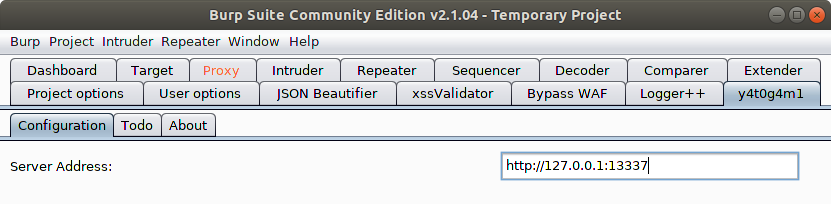
\includegraphics[width=\textwidth,keepaspectratio=true]{images/main-burp-extension-interface.png}
  \caption{Giao diện chính của phần mở rộng trên Burp Suite}
  \label{fig:main-burp-extension-interface}
\end{figure}
Sau khi khởi chạy công cụ webfuzzer và cài đặt phần mở rộng trên Burp Suite, ta tiến hành thiết lập proxy trên Burp Suite và trình duyệt web để bắt request mẫu như hướng dẫn tại \parencite{burp-suite-proxy}. Sau đó ta chuyển request mong muốn đến tab \texttt{Intruder} để tạo và gửi request mẫu đến máy chủ webfuzzer. Hình \ref{fig:send-base-request-1} mô tả quá trình này bằng cách thêm hoặc bỏ các kí tự ``\texttt{\$}'' bao quanh giá trị của tham số và chọn ``\texttt{Send to y4t0g4m1 webfuzzer}''.

Sau khi đã chọn loại lỗ hổng và gửi request mẫu đển webfuzzer, giao diện công cụ lần lượt hiển thị thông báo loại lỗ hổng sắp được kiểm thử (trong trường hợp này là \texttt{Time-based \acrshort{sqli}}) kèm theo các thiết lập của công cụ để phát hiện lỗ hổng đó, bao gồm tập tin chứa danh sách payload, đường dẫn chứa kết quả kiểm thử, các chuỗi dùng để so trùng trong response trả về, thời gian tối đa xử lí request. Sau đó là các kết quả kiểm thử đối với mỗi payload cụ thể và thông báo đã kiểm thử xong loại lỗ hổng này. Giao diện trong quá trình của kiểm thử của công cụ được thể hiện trong Hình 
Hình cũng thể hiện một số kết quả kiểm thử mà công cụ phát hiện thấy. Mỗi kết quả được in ra bao gồm các thành phần như sau.
\begin{itemize}
    \item \textbf{Kết quả kiểm thử} được đặt trong cặp ngoặc vuông, có thể là \texttt{[passed]} trong trường hợp payload khai thác thành công lỗ hổng, \texttt{[failed]} trong trường hợp payload không khai thác thành công hoặc \texttt{[skeptical]} trong trường hợp payload gây ra lỗi hoặc ngoại lệ khả nghi trong quá trình gửi request, chưa xác định được là có khai thác lỗ hổng thành công hay không, cần được hậu kiểm lại bằng tay.
    \item \textbf{Mã trạng thái HTTP} của response trả về, thường là \texttt{200} trong trường hợp request được gửi thành công hoặc các mã lỗi \texttt{401}, \texttt{404}, \texttt{500},... khi có sự cố trong quá trình xử lí request ở ứng dụng web mục tiêu.
    \item \textbf{Độ dài nội dung (content length)} của response trả về, \textbf{thời gian xử lí} của request tính theo giây và payload tương ứng được gửi theo request. Lỗi hoặc ngoại lệ trong quá trình xử lý request (nếu có) cũng được xuất ra ngay sau dòng kết quả kiểm thử.
\end{itemize}
Những kết quả kiểm thử được đánh dấu là \texttt{[passed]} hoặc \texttt{[skeptical]} sẽ được ghi lại trong nhật kí hoạt động kèm theo ngày giờ và loại lỗ hổng kiểm thử thành từng tập tin văn bản lưu trong thư mục \texttt{logs} trong đường dẫn gốc. Các tập tin nhật kí này chứa \acrshort{poc} khai thác lỗ hổng bao gồm request mẫu và các payload đã \texttt{[passed]} hoặc \texttt{[skeptical]} như Hình 
% TODO: Viết thêm hướng dẫn modify burp extension trong đây và trong README.md

\addcontentsline{toc}{chapter}{Tài liệu tham khảo}
% \bibliographystyle{alpha}
% \bibliographystyle{ieeetran}
% \bibliography{bibliography/bibliography}

\printbibliography

\end{document}